\documentclass[parskip]{cs4rep}

\usepackage{hyperref}
\usepackage{todonotes}
\usepackage[square]{natbib}
\usepackage[font=footnotesize]{caption}
\usepackage{subcaption}
\usepackage{amsmath}
\usepackage{copyrightbox}
\usepackage{forloop}
\usepackage{pdfpages}

\DeclareMathOperator*{\argmax}{arg\,max}
\DeclareMathOperator*{\argmin}{arg\,min}

\newcommand{\gene}[1]{{\tt #1}}
\newcommand{\histonemodification}[1]{#1}
\newcommand{\celltype}[1]{#1}
\newcommand*{\textprime}{\ensuremath{\prime}}
\newcommand{\pythonpackage}[1]{{\tt #1}}

\begin{document}

\title{Clustering and Visualisation\\ of DNA Sequencing Data}

\author{Saulius Lukauskas}

\degree{BSc Artificial Intelligence}
\project{Undergraduate Dissertation}

\date{\today}

\abstract{
\todo{Need an abstract}
}

\maketitle

%\section*{Acknowledgements}
%Acknowledgements go here.

\tableofcontents

%\pagenumbering{arabic}


\chapter{Biological Background}
This chapter summarises the biological background required to get to grips on what this honours project is about. 
A more in depth review of the topics discussed in this chapter could be find in molecular biology textbooks, for instance in \cite{Alberts:2002te}.

\section{DNA}

The complete set of information required to create and maintain cells of a
living organism is contained in the genome of the said organism. In humans, this
information is encoded in a long chain of nucleotides that form the DNA molecules. 
These chains of nucleotides can be sequenced by determining the order of appearance
of the four bases within the genome: adenine (often abbreviated as simply ``A"), cytosine (abbreviated as ``C"),
guanine (``G") or thymine (``T").
This sequence of nucleobases is what is commonly referred to as the DNA Sequence. 

\begin{figure}[p]
    \centering
    \copyrightbox{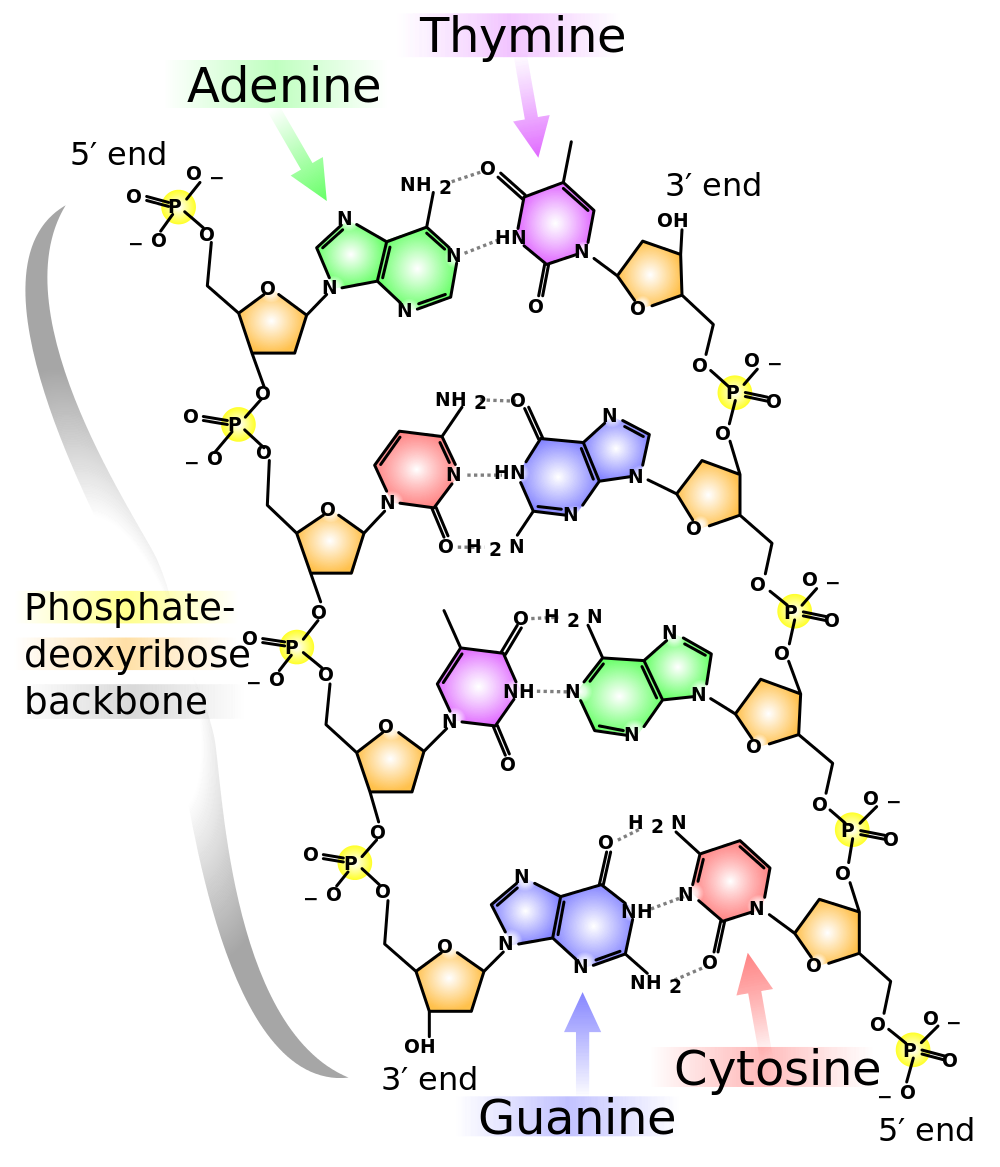
\includegraphics[height=0.35\textheight]{figures/background/DNA_structure.png}}
                 {Illustration from the Wikipedia Commons, released to public domain by the author.\\
                  Available at \url{https://simple.wikipedia.org/wiki/File:DNA_chemical_structure.svg}}
    \caption{Chemical structure of the DNA molecule. The two strands of DNA are being held together by the hydrogen bonds between adenine and thymine or guanine and cytosine, as pictured. Note that the strands have opposing chemical polarities, the end of a strand with a phosphate group (yellow) is often referred to as the $5'$ end, whereas the end with a deoxyribose group (orange) is commonly referred to as the $3'$ end.}
    \label{fig:background:dna_structure}
\end{figure}

Generally, DNA molecules are observed in pairs of two tightly connected molecules known as strands. These strands are held together by hydrogen bonds between the nucleobases: guanine is
known to form a bond with cytosine, whereas adenine forms a bond with thymine, as is illustrated in \autoref{fig:background:dna_structure}.

Both strands have opposing chemical polarities, determined by the position
of phosphate group (marked as yellow P in the figure) relative to the position of sugar group (deoxyribose in DNA, marked as orange pentagon). The end of the strand with a phosphate group is generally referred to as $5'$ end (the ``five prime end"), whereas the other end is referred to as $3'$ end, as labeled in the figure.

Since each kind of nucleobase can form a bond with only one other kind of
nucleobase, both of the DNA strands contain enough information to recreate the
other on its own, a crucial property that allows DNA to replicate. 

Because of this redundancy, the sequences on both strands can be sequenced simultaneously, therefore sequences of nucleotides are often referred to in terms of base pairs (abbreviated as bp.), rather than individual nucleotides. Human sex cells are known to contain around three billion such base pairs, other cells containing twice the amount \cite{Annunziato:2008wh}.

\begin{figure}[p]
   \centering
   \copyrightbox[b]{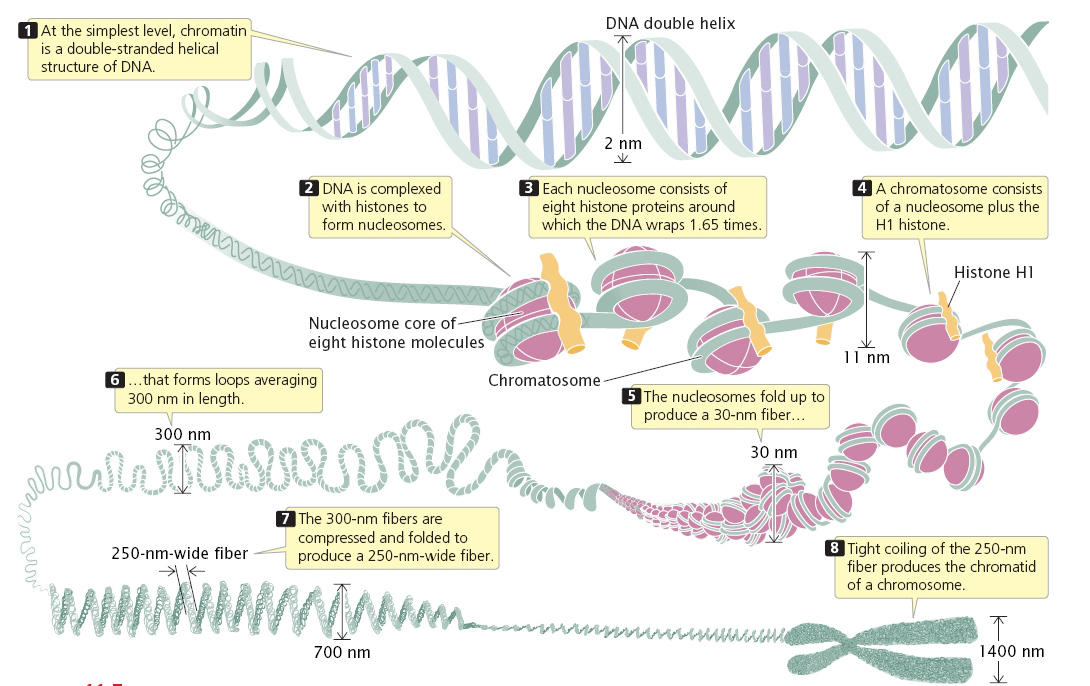
\includegraphics[height=0.40\textheight]{figures/background/pierce_11_5_FULL.jpg}}
   {Copyright 2005 W. H. Freeman Pierce, Benjamin. Genetics: A Conceptual Approach, 2nd ed. (New York: W. H. Freeman and Company), 292. Sublicensed by Scitable to be used in print for non-commercial use in an educational environment (via \cite{Annunziato:2008wh}).}
   
   \caption{Infographics of DNA Packaging mechanism. }
   \label{fig:background:dna_packaging} 
\end{figure}

Since each base pair in the DNA is around 0.34 nanometers long \cite{Annunziato:2008wh},
DNA sequence of a human diploid cell will take up around 2 meters in length, if stretched, yet it is packaged into a volume as small as the nucleus of a cell. This packaging is done with the help of proteins called histones that fold the DNA around them, eventually wrapping it into three dimensional structures.

More specifically, DNA wraps around an octomer of two copies of each of the four core histones, creating a structure resembling beads on a string that is pictured in panels 2 and 3 of \autoref{fig:background:dna_packaging}. These core histones are known as histones H2A, H2B, H3, and H4.
The fifth histone, H1, attaches itself to the DNA from the opposite side to the other histones, as pictured in yellow in the panel 4 of figure \ref{fig:background:dna_packaging}. The segment of DNA and the histone it is wound around, is known as nucleosome. These nucleosomes are then further wrapped into a structure known as the 30-nanometer fibre, which is then  wrapped to even higher order structures, as seen in \autoref{fig:background:dna_packaging}. The warped combination of DNA and the proteins inside the nucleus of a cell is commonly referred to as the chromatin.

These DNA-wrapping histones are known to be mostly modular in structure, with a number of ``tails" that are susceptible to chemical modifications such as methylation, acetylation and phosphorylation \cite{Fischle:2003tl,Kouzarides:2007js}. These chemical modifications on histone tails have been shown to be able to alter the structure of chromatin. For instance, acetylation of histone H4 on lysine 16 (shortened as \histonemodification{H4K16Ac}, where \emph{H4} is the histone number, \emph{K16} stands for lysine 16 and \emph{Ac} stands for Acetylation) has been shown to inhibit formation of the 30-nanometer fibre \cite{ShogrenKnaak:2006gt}. These changes of the chromatin structure can affect the accessibility of the DNA. Intuitively, the tighter DNA is packaged, the less accessible it is to various chemical interactions.

\section{Gene Expression}
\begin{figure}[t]
\centering
\copyrightbox[b]{
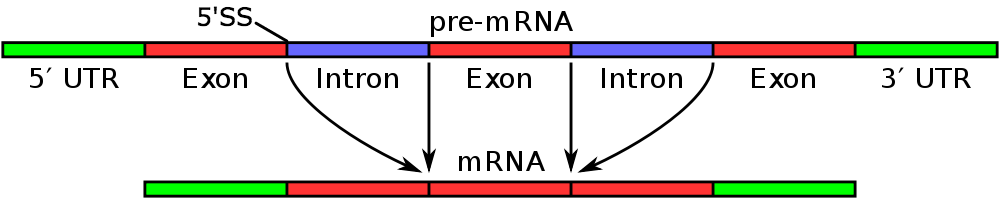
\includegraphics[width=\textwidth]{figures/background/gene_splicing.png}}
{\centering Modified version of \url{https://en.wikipedia.org/wiki/File:Pre-mRNA_to_mRNA.svg}. The original image was released to the public domain.}
\caption{RNA splicing}
\label{fig:background:splicing}
\end{figure}

Gene expression process can be summarised using the central dogma of molecular biology: 
\emph{DNA makes RNA makes proteins}. Technically speaking, gene expression is a combination of two processes, transcription (DNA to RNA) and
translation (RNA to protein) which produce a functional product of a gene, e.g. a protein\footnote{Not all genes produce proteins as their functional product. For the sake of simplicity, these so called non-coding genes are not discussed in this chapter.}.

During transcription, RNA polymerase molecule binds to a region of DNA that is indicated by a complex ensemble of proteins bound to promoter regions of DNA. This molecule then proceeds to read information encoded in one of the strands, synthesising RNA molecule complimentary to the nucleotides read. The strand that was read by RNA polymerase molecule is commonly referred to as the template or antisense strand, and is read in direction from $3'$ end to $5'$ end, meaning that the RNA molecule is created from $5'$ end to $3'$ end. Since the generated RNA is complimentary to the sequence on the template strand, it will have exactly the same arrangement of nucleotides, as in the remaining strand\footnote{The only exception being that in RNA molecule thymine is replaced with uracyl.}. Due to this reason the remaining strand is often referred to as the coding or sense strand.

Even though the complete length of the gene is transcribed into RNA, only a fraction of it is translated to the protein. Fragments of gene, known as introns, are removed post transcription by the process known as RNA splicing. The remaining regions, exons, are then joined and form the final messenger RNA. This process is schematically illustrated in \autoref{fig:background:splicing}. The regions between exons and introns are known as splicing sites. 

After splicing, the resulting messenger RNA (mRNA) is transferred to the ribosome, that will create the proteins from the blueprint encoded inside the mRNA. A more in depth view of these processes can be found in a molecular biology textbook, e.g. in \cite{Alberts:2002te}.

Gene expression is particularly interesting for epigeneticists, who are concerned about the factors that may alter it without altering the underlying DNA sequence. Chemical histone modifications have been shown to correlate with the transcriptional activity of the genes near them \cite{Pokholok:2005wn,Kouzarides:2007js}, making them an interesting topic of research for epigeneticists. The next section summarises the methods designed to study them. 
 
\section{Next-Generation Sequencing}

It took 13 years and around \$2.7 billion to sequence the whole human genome for the first time, by the scientists of the Human Genome Project\footnote{For more information, see \url{http://www.genome.gov/11006943} and
    \url{http://www.ornl.gov/sci/techresources/Human_Genome/project/about.shtml}}. 
    
    
\begin{figure}
    \centering
    \copyrightbox[b]{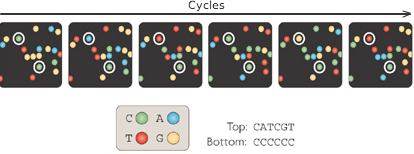
\includegraphics[width=0.8\textwidth]{figures/background/IlluminaSequencing.png}}
    {Adapted by permission from Macmillan Publishers Ltd: Nature Reviews Genetics,
     Michael L. Metzker, \emph{Sequencing technologies — the next generation}, copyright 2010 (\cite{Metzker:j6NWuwFp})}
    \caption{Illustration of parallel sequencing of nucleotides, as in Illumina/Solexa Sequencing platform.
    Each coloured dot in the figure corresponds to a different fragment of DNA being sequenced. 
    At each cycle, colour-coded nucleotide is incorporated to DNA by a mechanism similar to DNA replication. Then imaging is performed to get the sequences of all the pieces of DNA all at once, resulting in an image similar to the one in this figure. For each DNA fragment, the colour is read and mapped back to the nucleotide. The dyes are then washed and the cycle continues \cite{Metzker:j6NWuwFp}.}
    \label{fig:background:ngs:illumina}
\end{figure}

Since then, the cost and duration of DNA sequencing has dropped sharply with the invention of
the Next-Generation Sequencing methods (NGS). Instead of sequencing a long segment of DNA sequentially,
the next-generation sequencing methods sequence a lot of short DNA segments in a massively-parallel way, much like as depicted in \autoref{fig:background:ngs:illumina}.

The short-sequenced reads can then be put together via the overlapping fragments between the reads. Anyone who ever tried solving a puzzle without looking at the cover, knows how hard this process could be, even for computers. That is why NGS methods that produce very short reads are usually used not for tasks of sequencing the genome for the first time (\emph{de-novo} sequencing), but
rather to study the DNA itself.

\section{ChIP-Sequencing}
\label{sec:chip}

\begin{figure}
\centering
\copyrightbox{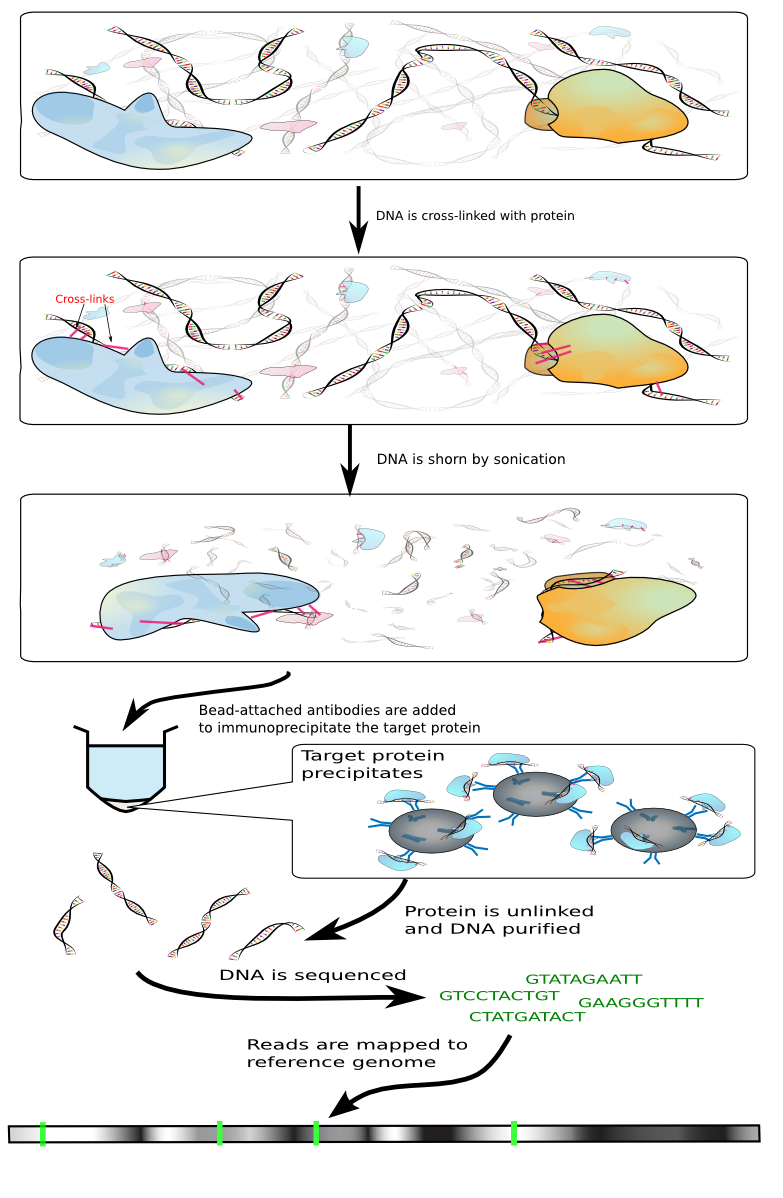
\includegraphics[height=0.8\textheight]{figures/background/ChIP-Seq.png}}
{Adapted from \url{https://en.wikipedia.org/wiki/File:Chromatin_immunoprecipitation_sequencing.svg}.
The original document was licensed under Creative Commons Attribution-Share Alike 3.0 Unported license}
\caption{ChIP Sequencing workflow. First, the target proteins are cross-linked with DNA. This DNA-Protein complex is then shorn into smaller pieces by sonication. Antibodies for the target proteins are added to mixture in order to immunoprecipitate it. The precipitate containing the target protein is collected and purified to extract DNA. This DNA is then sequenced and mapped to reference genome.
}
\label{fig:background:chip}
\end{figure}

Chromatin Immunoprecipitation, followed by Sequencing (ChIP-Seq) is a NGS method that studies protein-DNA interactions within the cell. Instead of sequencing the whole genome, ChIP-Seq aims to sequence only parts of DNA that interact with some target protein. These target proteins can either be internal to DNA (histones) or arbitrary external proteins that interact with DNA.

Basic ChIP-Seq workflow is summarised in \autoref{fig:background:chip}. In short, proteins are first ``glued" together with the DNA by chemical cross-linking. This DNA-with proteins attached to it is then shorn into smaller pieces. Antibodies are added to single the target proteins out using immunoprecipitation. Precipitate is then collected and the DNA that is attached to the target proteins is sequenced. This sequenced DNA is then matched to the reference genome to provide hints of which parts of genome interact with the protein \cite{Mardis:2007wa}.

\begin{figure}[t]
    \centering
    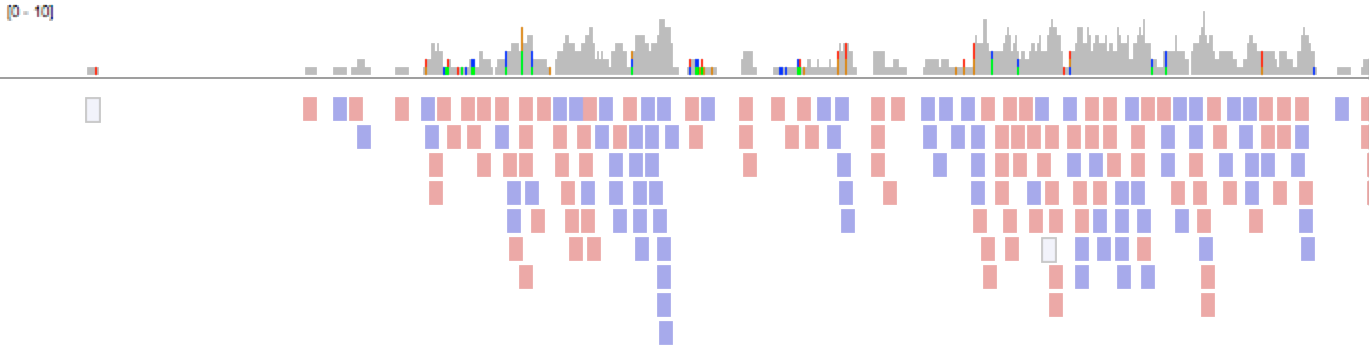
\includegraphics[width=\textwidth]{figures/background/igv_panel_screenshot_k562_h3k4me3_WDTC1-transparentbcg.png}
    \caption{A typical result of ChIP-Seq experiment. Pictured here is the region around the transcription start site for gene \emph{WDTC1} (chr1:27,559,006-27,563,006). The experiment targeted histone modification \histonemodification{H3K4Me3} in cell type \celltype{K562} from ENCODE dataset (see \autoref{sec:datasets}). The aligned reads are pictured as rectangles with colour indicating the directionality. The histogram, often referred to as the, in this case \histonemodification{H3K4Me3}, mark is computed by calculating the number of reads that overlap particular base pair. The image was generated by taking a screenshot of Integrative Genomics Viewer (IGV) \cite{Thorvaldsdottir:2012wy}.}
    \label{fig:background:chip-results}
\end{figure}

Figure \ref{fig:background:chip-results} shows a typical result of ChIP-Sequencing experiment.
The aligned reads are pictured as rectangles below the histogram. Usually only a short fragment of DNA attached to protein (e.g. 36 base pairs) is sequenced. In most cases, the sequencing is done from $5'$ end to $3'$ only\cite{Park:2009wc}. This means that the DNA that was read from the reverse strand will have opposite direction than the DNA that was read from the forward strand. This directionality is then recorded and can be used to correct some of the sequencing artefacts, as described in \autoref{sec:reading_and_preprocessing}.

The aligned reads are then stacked together into a histogram, creating a landscape of target protein enrichment, as seen in \autoref{fig:background:chip-results}. These enrichment landscapes, often referred to as just ``marks", are then analysed computationally in order to gain insights on the role the target proteins play in the living organisms. Even though these marks are technically histograms of the number of reads falling within the region, they are commonly visualised as continuous functions, for the sake of simplicity.

Chapter \ref{cha:motivation} reviews the common computational approaches of exploring this data, as well as gives motivation on the approach taken by the author.

\subsection{Publicly available Datasets}
\label{sec:datasets}

Before jumping to the motivation for the project, it is important to note the publicly available datasets of ChIP-Seq experiment results.

The Encyclopedia of DNA elements, ENCODE, \cite{TheENCODEProjectConsortium:2004db} has compiled a large collection of histone modification data from the Broad Institute (\url{https://www.broadinstitute.org/}). This data is publicly available to download and use via the ENCODE website at \url{http://genome.ucsc.edu/cgi-bin/hgFileUi?db=hg19&g=wgEncodeBroadHistone}. 

This project uses these publicly available datasets in all of it's experiments and some of the figures. Unless explicitly stated otherwise, the ENCODE ChIP-Seq datasets for K562 leukaemia cell line are used in this project.

Whenever the annotated locations of known genes, transcription start sites, and first-splicing sites are used, they are used from the UCSC Known Genes collection \cite{Hsu:2006dh} (hg19 assembly), and are free to download via the ENCODE table browser. 

This track assigns a unique 10-character id, e.g. \gene{uc003vhn.1}, for each of the genes and their variants. These identifiers are referenced in the text of the report whenever possible, and they can be used to query the UCSC Genome browser \cite{Kent:2002wd} directly, if it is desired.

\chapter{Motivation}
\label{cha:motivation}

In one of the early reviews of ChIP-Seq, \cite{Park:2009wc}, P J Park already predicted data processing to be the major challenge of this technology, and therefore listed the most common approaches to data processing at that time. Almost four years later today, most of these approaches still remain valid.

For protein-DNA binding, he writes, the most common analysis is the discovery of the short segments of DNA the protein is most likely to bind to, so called binding sequence motifs. A large variety of methods to do that are available today, probably the best-known one being MEME \cite{Grundy:1997vb}.

In order to find these transcription factor binding sites, significantly enriched regions of the genome (so called "peaks") need to be located first. MACS peak caller \cite{Zhang:2008wp} is the method of choice for this task to date, even though a variety of other methods have been proposed since (see \cite{Furey:2012ha} for a recent review).

\begin{figure}[p]
   \centering
   \copyrightbox{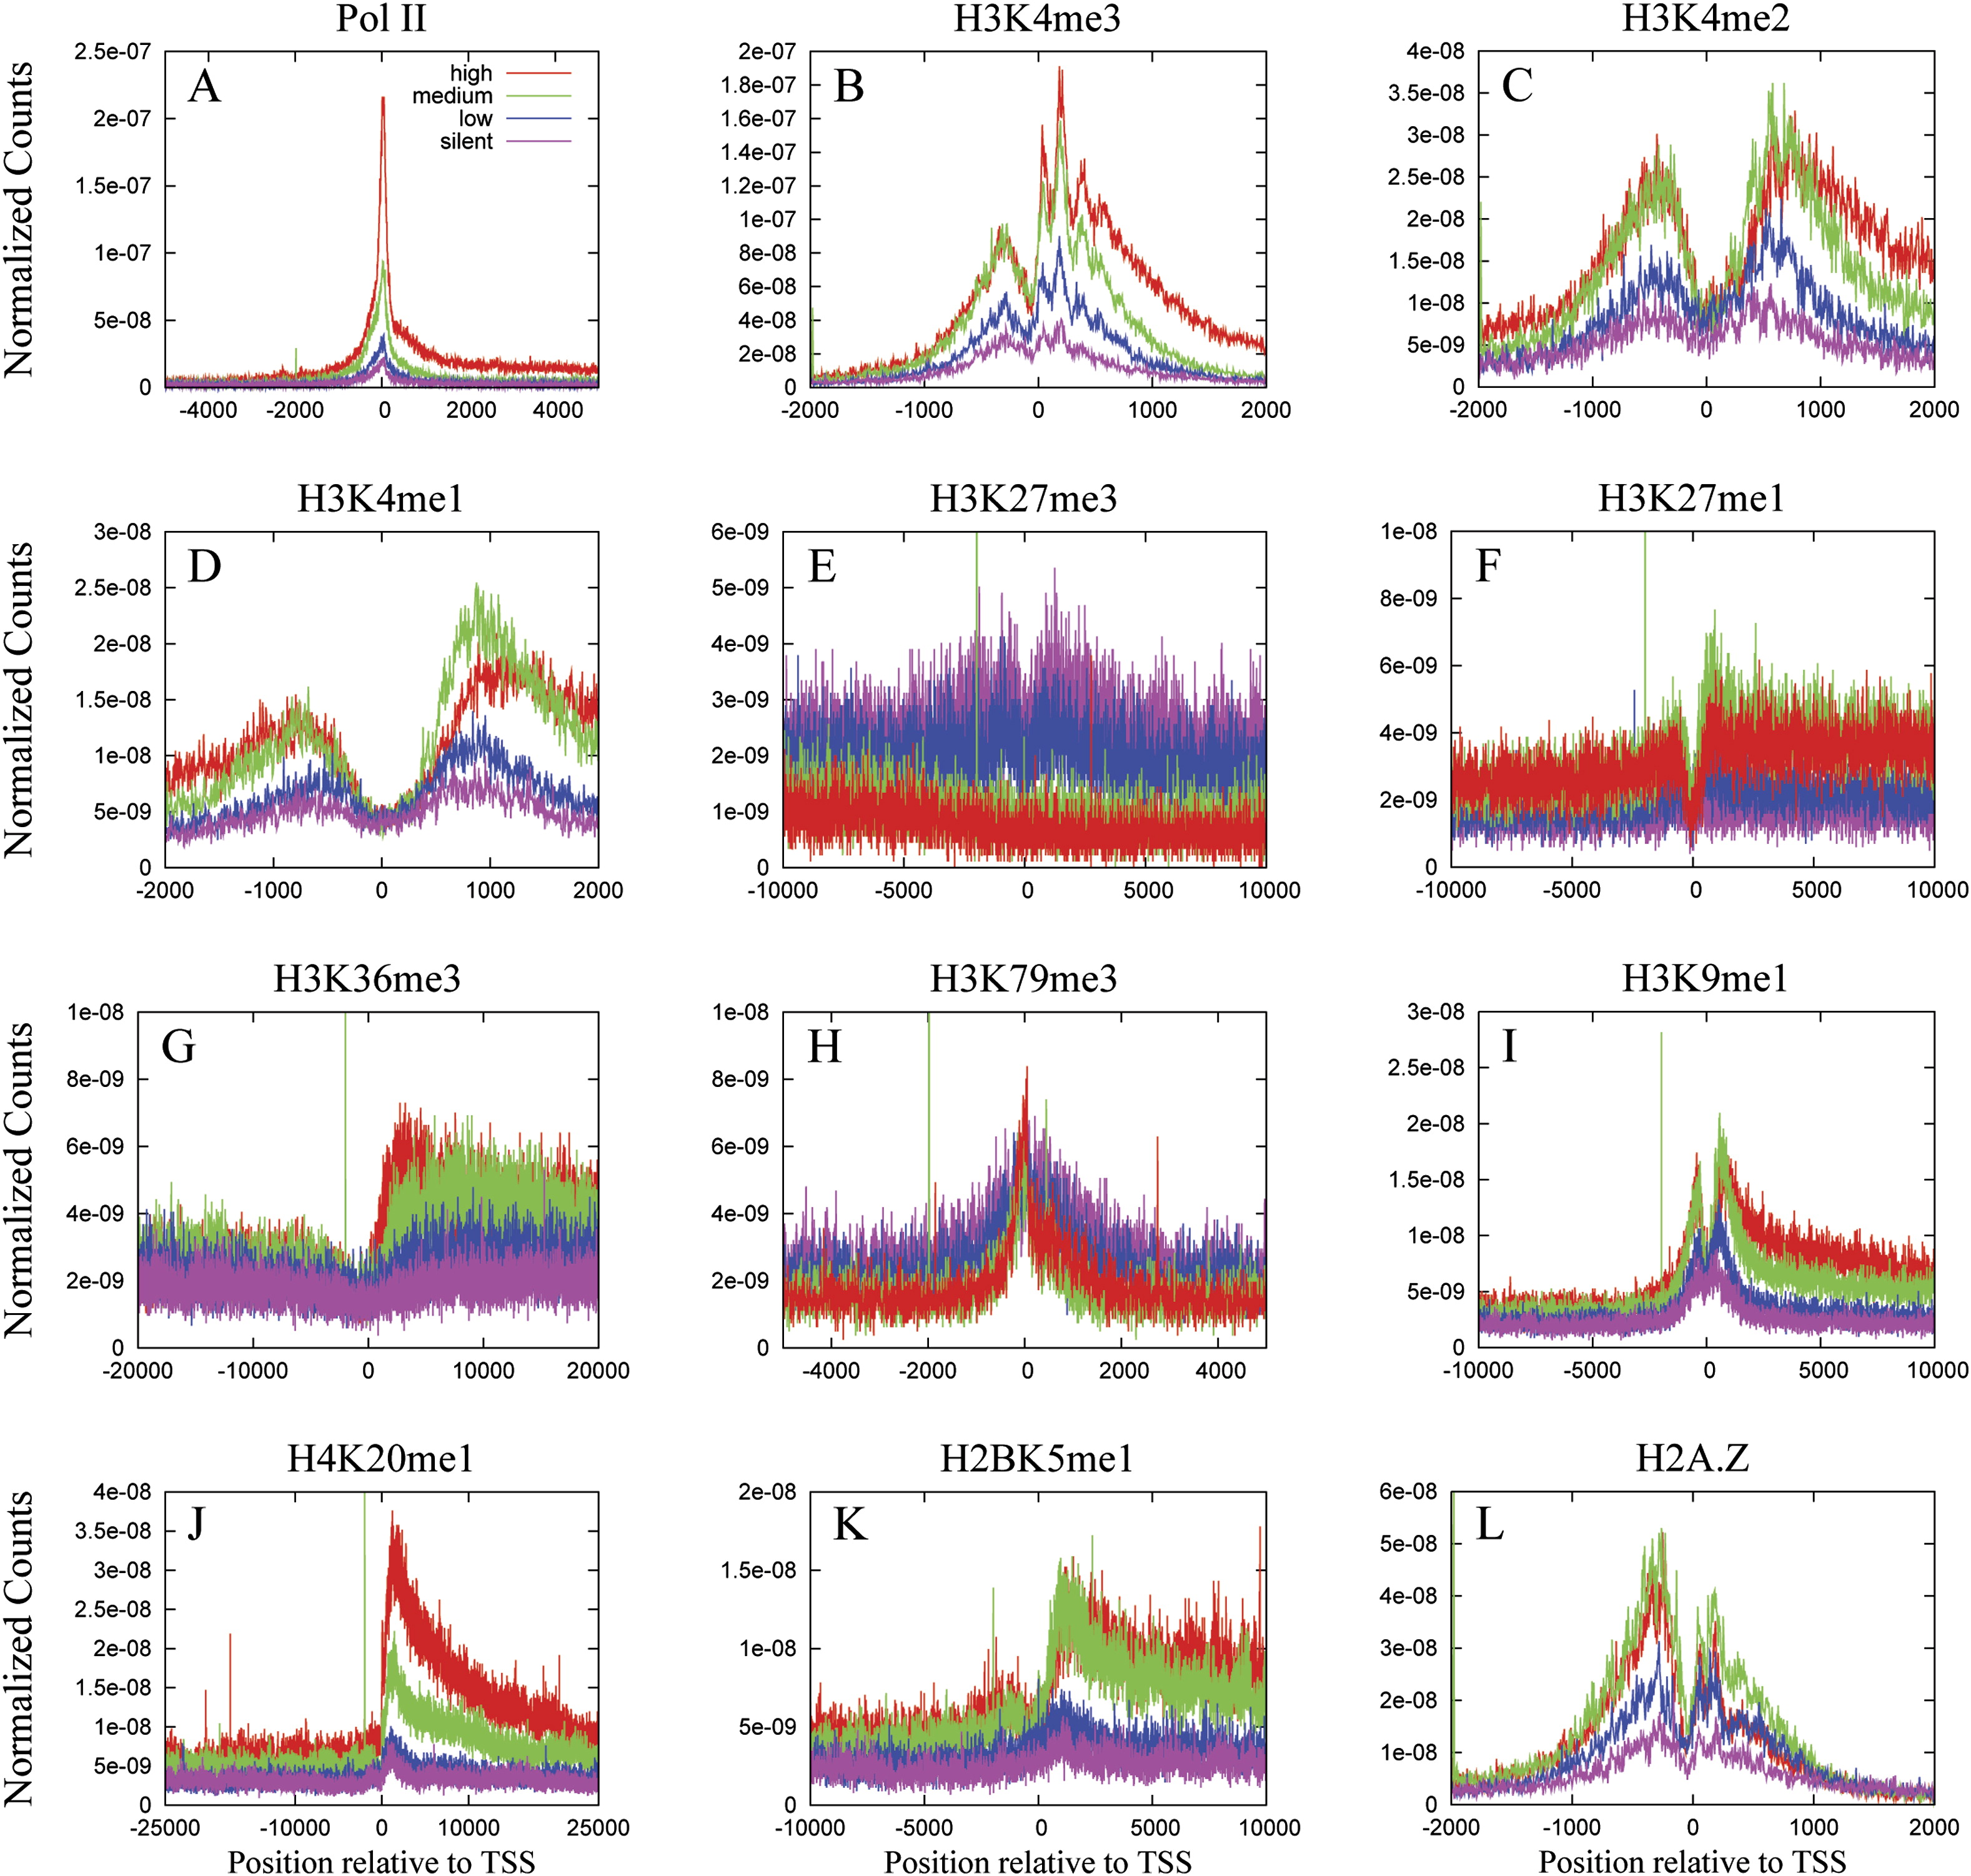
\includegraphics[width=\textwidth]{figures/motivation/barski-histone-modifications-around-tss.jpeg}}
   {Reproduced from Cell, 129, Artem Barski, Suresh Cuddapah, Kairong Cui, Tae-Young Roh, Dustin E. Schones, Zhibin Wang, Gang Wei, Iouri Chepelev and Keji Zhao, High-Resolution Profiling of Histone Methylations in the Human Genome\cite{Barski:2007ww}, p. 826, Copyright 2007, with permission from Elsevier}
   \caption{Profiles of histone marks around known transcription start sites. The profiles for highly active, two stages of intermediately active and silent genes are colour-coded. The histone modification is shown on top of each plot. ``Normalized counts" on the Y axes refers to the normalised number of reads obtained from ChIP-Seq experiment that overlap a particular bin. The results were compiled by \cite{Barski:2007ww}.}
    \label{fig:motivation:histone_profiles}
\end{figure}

For histone modification studies, an obvious approach, as claimed by P J Park, is to annotate the locations of these peaks relative to known genomic features. For instance, it has been observed
that, on average, histone modifications have very distinct bimodal marks near transcription start sites, as pictured in \autoref{fig:motivation:histone_profiles}. It is also noted that most of the marks, e.g.
\histonemodification{H3K4me3} mark, correlate with the activity of genes being analysed: highly active genes (red in the figure) have more reads falling within the same region than intermediately active ones (green and blue) \cite{Barski:2007ww}.

What is more interesting, these histone marks are so distinctive, that 
\cite{Heintzman:2007ke} were able to predict locations of regions that both initiate (promote) and enhance transcription of DNA by training a classifier on a combination of histone marks around known promoter and enhancer regions. Later, \cite{Hon:2008wv} developed a method called ChromaSig, that was able to find the promoter and enhancer signatures in completely unsupervised way by simply looking at the most common histone mark motifs within the genome.

However, the fact that ChIP-Seq signal can tell us more than just the type of DNA region is more interesting. In the already mentioned paper, \cite{Barski:2007ww}, the authors note: ``A series of peaks of H3K4me3 signals at +50, +210, and +360 were detected, suggesting similar nucleosome positioning relative to TSS in active genes"\footnote{Original text misspells \emph{H3K4me3} as \emph{H4K4Me3}}, these peaks can be seen in figure \autoref{fig:motivation:histone_profiles}. This claim was later followed-up by \cite{Schmid:2007ue}, who were able to locate promoter-specific nucleosomes ``with unprecedented precision" from this ChIP-Seq data.

Another, very recent paper by Bieberstein and colleagues \cite{Bieberstein:2012tf} has shown that \histonemodification{H3K4Me3} and \histonemodification{H3K9Ac} profiles tend to peak at the locations of $5'$ splicing sites of known genes. The authors also conclude that these peaks are independent of nucleosome positioning, unlike the peaks observed by \cite{Barski:2007ww}.

An important point to take away from these two results is that insights to underlying biological processes can be produced from the visual inspection of these histone marks. This observation is the main source of motivation for this project. 

The ultimate goal of this project is to develop a tool that would allow to group similar patterns into clusters and provide means to visually compare these patterns on a common ground, so hypotheses about their origin could be made.

\section{Prior art}

There have been a few prior attempts at clustering these histone marks.
The already mentioned ChromaSig method (\cite{Hon:2008wv}) aims to find the patterns that commonly occur in the genome, by aligning various segments of genome to each other. Another paper, \cite{Lai:2010ue}, uses a similar alignment method to align patterns from user-supplied regions in the genome, so they can then be visually compared on the same ground.

While both of these methods would probably succeed in detecting the patterns that occur at relatively uniform intervals, e.g. patterns that occur due to nucleosome positioning, both of them would struggle to provide the splicing site insights documented in \cite{Bieberstein:2012tf}. The vastly varying lengths of first exons call for non-linear scaling of the genomic regions to align them.

Also, in some cases, alignment without any kind of scaling, does not make any sense at all. For instance, if one was about to compare the regions spanning whole lengths of known genes, the best these methods could do is to compare a small fragment of the longer gene to the complete length of the shorter one, which is not necessarily the correct thing to do. 

This is the reason why some studies, e.g. \cite{Taslim:vj}, rescale the regions of interest to be of the same length, before doing clustering. This could indeed allow visualisation of similar patterns between the different regions, provided that these patterns scale linearly with the length of the regions, yet most likely this is not the case.

Essentially, this problem of comparing genomic patterns of varying lengths is very similar to the problem of comparing waveforms of spoken words in speech recognition. 
For instance, it is desired to identify two words being the same even though the recording for one of them started, say half a second later. Equivalently, it is desired to detect patterns that are similar, but misaligned. Furthermore, a good speech recognition system would be able to recognise a word correctly even though the speaker prolonged one of the vowels in the word more than it usual, what is similar to patterns that are influenced by the length of the first exon.

Fortunately, the speech recognition community has already matured an approach to this problem. This approach, called Dynamic Time Warping (or simply, DTW), compares two sequences by shrinking or expanding both of them non-uniformly to be as similar as possible. This non-linear warping can then both account for misalignment, by shrinking the misaligned part of one of the sequences, and scaled patterns, by rescaling them to be of the same length. This project proposes a method that combines this Dynamic Time Warping distance with hierarchical clustering with the aim of comparing genomic features. Instead of using Dynamic Time Warping to compare time-series data, it is directly used to compare the genomic data. Due to this reason, this new method is named Dynamic Genome Warping or simply DGW.

In its essence, this method is very similar to the ChAT method, described in \citep{Wang:2012cb}.
This method tries to find the best alignment between two patterns before doing any clustering, just as ChromaSig or ArchAlign, yet it allows to ignore a part of some region as if it was not there. The authors of the paper claim that these gaps ``are critical because they allow the algorithm to extend beyond regions with variant (or diffuse) chromatin enrichment signatures, and in so doing facilitate the discovery of chromatin signatures that span long genomic regions as well as those with complex multi-modal patterns of histone modification enrichment". 

The main difference between the method used in this project and the one used by Wang et al. is that when creating gaps, ChAT algorithm applies a penalty that is proportional to the norm of the vector that is being skipped. Such penalty biases the algorithm to skip unexpressed regions more than expressed ones as per reasoning that depleted regions are not as interesting as the expressed ones. 
While this penalty allows the discovery of multi-modal patterns separated by depleted regions across genome, it would heavily penalise any attempts to discover patterns of varying lengths in highly-expressed regions.

Contrary to this, the DTW distance measure does not allow skipping of the points at all. It does, however, allow a set of points on one sequence to a single point on another as if that point was stretched to become a sequence of n points. This way the penalty of warping the genome depends directly on the points that are aligned to each other, so the algorithm is able to do this both for highly expressed and fairly depleted regions, as long as the values mapped to each other are similar.

\todo{write about how chat method was developed independently of this one}

The exact workings of DGW are explained in detail in the next chapter.

\chapter{Methods}
\section{Dynamic Time Warping}
\label{sec:DTW}

\begin{figure}[b,t]
   \centering
   \begin{subfigure}[b]{0.45\textwidth}
       \centering
       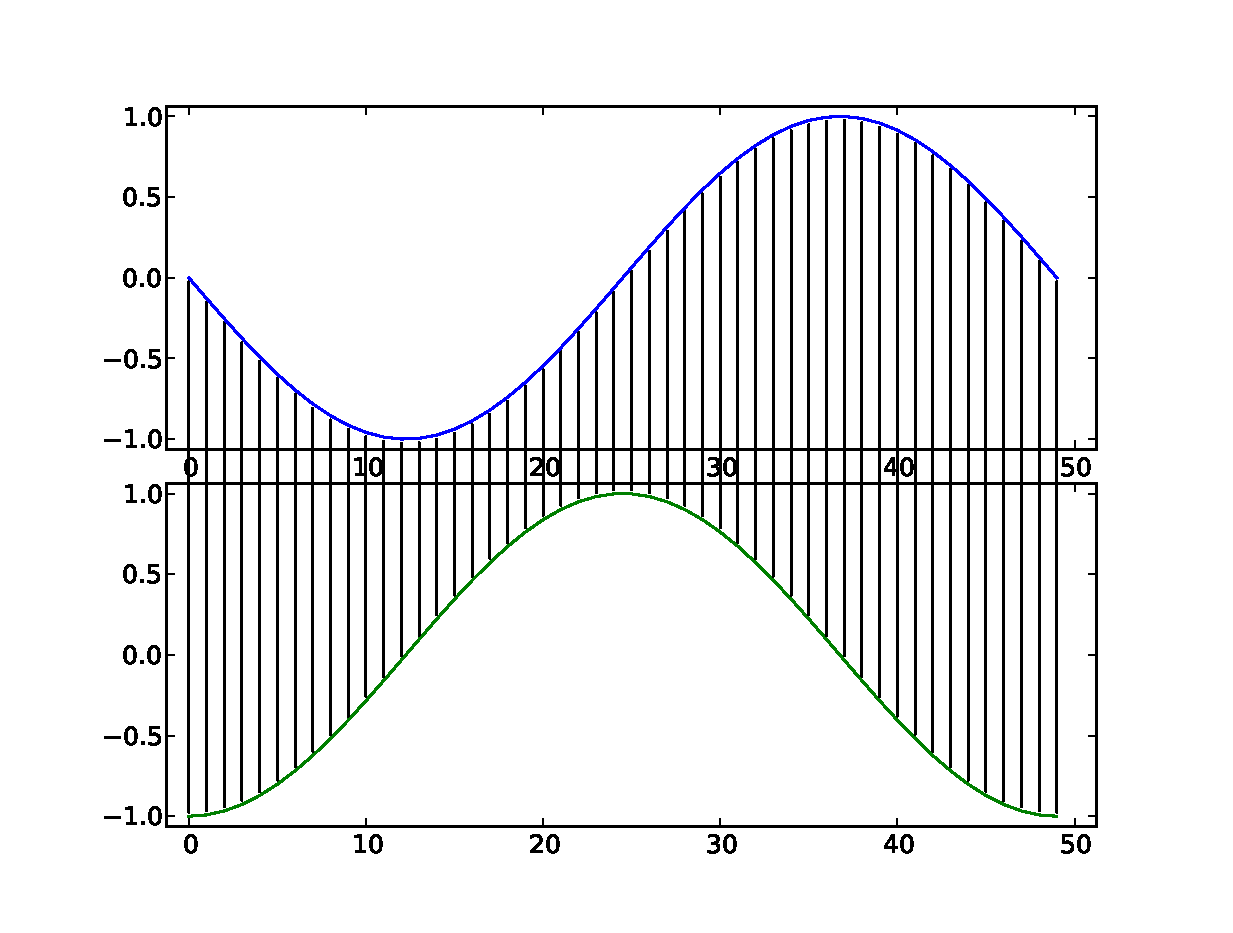
\includegraphics[width=\textwidth]{figures/DTW/sin-cos-no-dtw.eps}
       \caption{Euclidean alignment}
       \label{fig:DTW:euclidean_alignment}
   \end{subfigure}
   ~
   \begin{subfigure}[b]{0.45\textwidth}
       \centering
       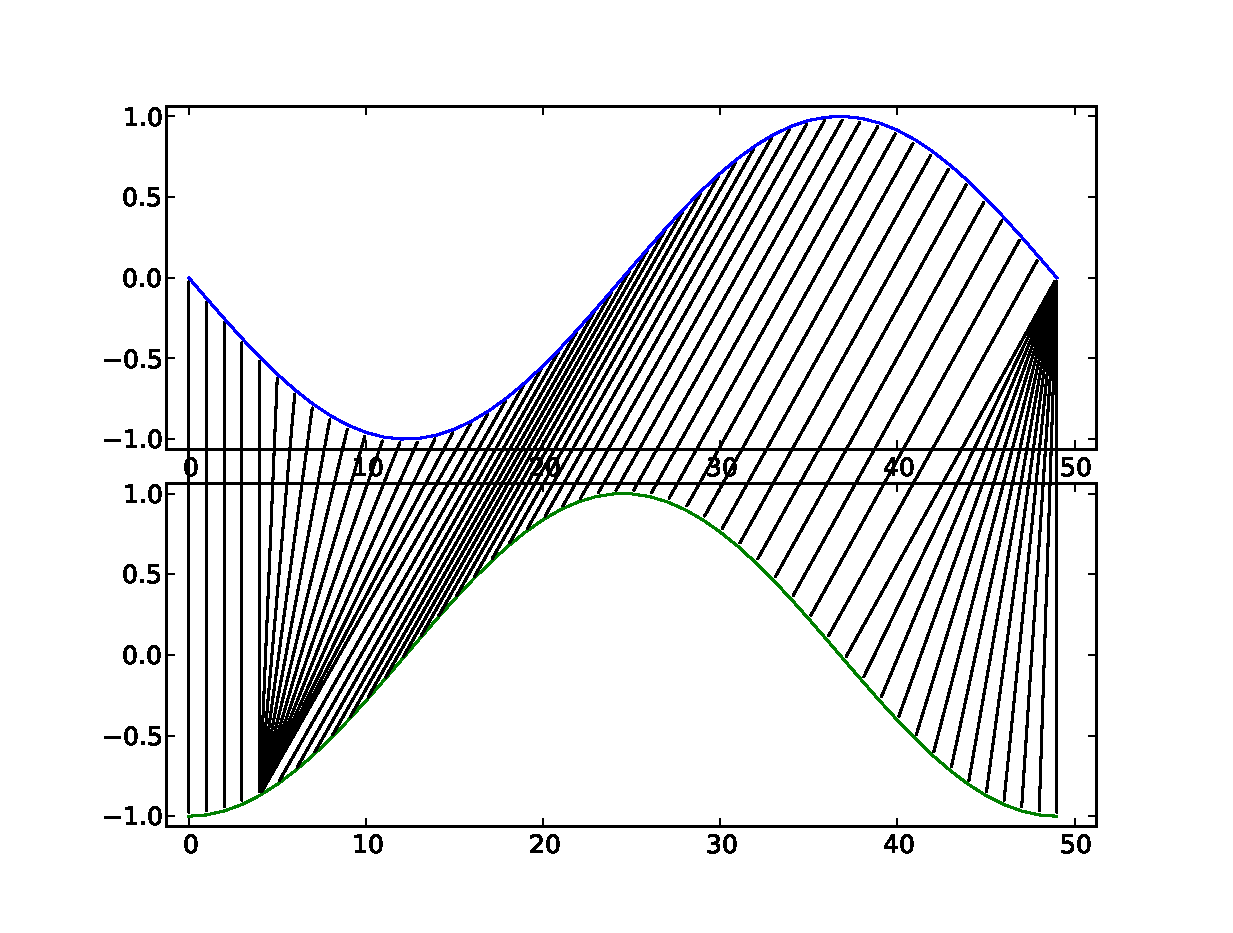
\includegraphics[width=\textwidth]{figures/DTW/sin-cos-dtw.eps}
       \caption{DTW alignment}
       \label{fig:DTW:dtw_alignment}
   \end{subfigure}
   
   \caption{Two sequences aligned to each other. Figure \ref{fig:DTW:euclidean_alignment} maps each point on sequence A to a point on sequence B directly, resulting in an Euclidean distance measure, whereas figure \ref{fig:DTW:dtw_alignment} uses Dynamic Time Warping algorithm to find a better mapping between the points.}
   \label{fig:DTW:alignments}
\end{figure}

Dynamic Time Warping (DTW) algorithm is the corner stone of this project. This algorithm was initially developed in the speech recognition community in order to allow accurate comparisons between words spoken with tempo variations. 

This comparison is achieved by warping the time axis nonlinearly. That is, the axis is stretched or compressed as to minimise the total distance between the points aligned to each other. The stretching and compressing is done by creating an alignment between the two sequences, also known as the warping path, almost arbitrarily, with a few constraints described below. The distances between aligned points are then computed and summed up to obtain what is commonly referred to as DTW Distance.

More formally, given two sequences $\mathbf{a} = a_1, a_2, ..., a_n$ and $\mathbf{b} = b_1, b_2, ..., b_m$, Dynamic Time Warping aims to construct a warping path\\
$\mathbf{p} = { (p_{1,0}, p_{1,1}), (p_{2,0}, p_{2,1}), ..., (p_{k,0}, p_{k, 1}) }$ that maps each point on the first sequence, specified as $p_{i,0}$ to a point on the second sequence, $p_{i,1}$, such that the following three constraints hold:

\begin{enumerate}
\item \emph{Boundary Condition}: The path must start at the first point of sequence $\mathbf{a}$ and this point must be mapped to the first point of the second sequence: $p_1 = (1,1)$. Similarly, the final points of both sequences should be mapped to each other, and the path must end there: $p_k = (m, n).$ 
\item \emph{Monotonicity Condition}: The path must not move \emph{back in time}: 
    $p_{1,i} \le p_{2,i} \le p_{3,i} \le ... \le p_{k, i}$ for both $i=0$ and $i=1$.
\item \emph{Step Size Condition}: At each step the path must either map the same point on one sequence to the next point on another sequence, or map next points on both sequences together, mathematically:
    $p_{i+1} - p_{i} \in \{(0,1), (1,0), (1,1)\}$ for all $i < k$.
\end{enumerate}

The problem is to find a warping path that is minimal, given some distance measure $d$ that would compute the distances between aligned points (e.g. Euclidean distance): $\hat{P} = \argmin_P \sum_{(i,j) \in P} d(a_i, b_j)$.

Such minimal warping alignment can be computed in $O(nm)$ time by applying dynamic programming techniques. 

Specifically, we construct a $n \times m$ matrix $\mathbf{D}$ where each entry $D_{i,j}$ will contain a minimal (warped) distance of matching first $i$ components of the first sequence, $a_1..a_i$, to first $j$ elements of the second sequence, $b_1..b_j$. The first component of the matrix, $D_{1,1}$ is initialised to the distance between the first components of the two sequences, $d(a_1, b_1)$ as specified by the boundary condition.

The matrix is then filled row by row, according to the following recursive equation:
\begin{equation}\label{eq:dtw_equation}
D_{i,j} = d(a_i, b_j) + min(D_{i-1, j}, D_{i, j-1}, D_{i,j})
\end{equation}

In the end, the column $D_{n,m}$ holds the minimal warped distance between two series.
If the minimal warping path is needed, it can be traced back by following the recursive relation backwards from $D_{i,j}$. This algorithm is illustrated in \autoref{fig:DTW:example}. 

More information on the workings of DTW can be found in e.g. \citep{Muller:2007bo}.

\begin{figure}
   \centering
   \begin{subfigure}[b]{0.3\textwidth}
       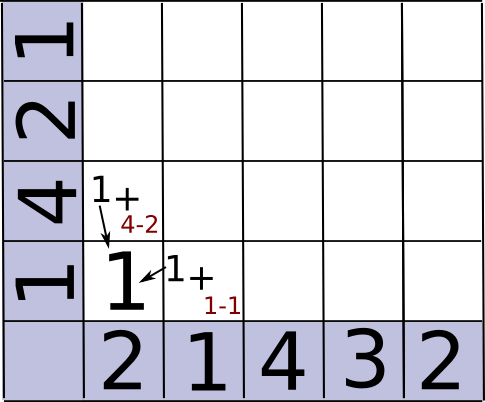
\includegraphics[width=\textwidth]{figures/DTW/worked-out/step-1.png}
       \caption{}
       \label{fig:DTW:example:1}
   \end{subfigure}
   ~
   \begin{subfigure}[b]{0.3\textwidth}
       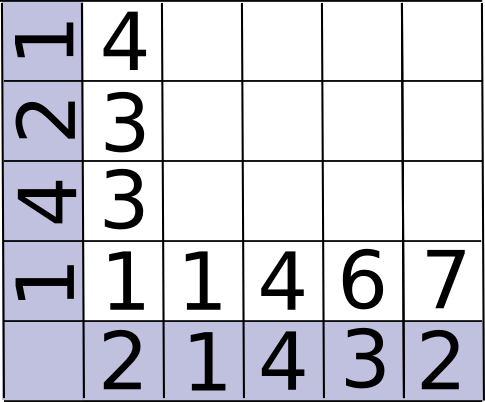
\includegraphics[width=\textwidth]{figures/DTW/worked-out/step-2.png}
       \caption{}
       \label{fig:DTW:example:2}
   \end{subfigure}
   ~
   \begin{subfigure}[b]{0.3\textwidth}
       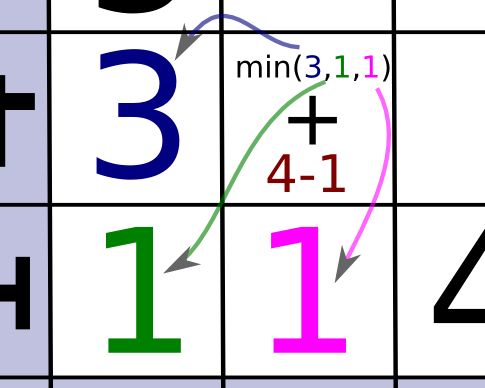
\includegraphics[width=\textwidth]{figures/DTW/worked-out/step-3.png}
       \caption{}
       \label{fig:DTW:example:3}
   \end{subfigure}
   ~
   \begin{subfigure}[b]{0.3\textwidth}
       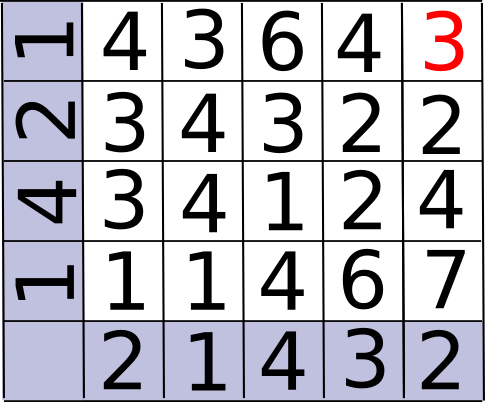
\includegraphics[width=\textwidth]{figures/DTW/worked-out/step-4.png}
       \caption{}
       \label{fig:DTW:example:4}
   \end{subfigure}
   ~
   \begin{subfigure}[b]{0.3\textwidth}
       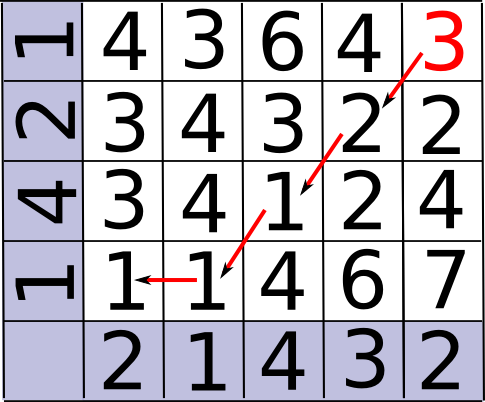
\includegraphics[width=\textwidth]{figures/DTW/worked-out/step-5.png}
       \caption{}
       \label{fig:DTW:example:5}
   \end{subfigure}
   ~
   \caption{Illustration of the DTW algorithm. Two sequences, $(2,1,4,3,2)$ and $(1,4,2,1)$ are being compared here using Euclidean distance. The algorithm first creates an empty table of size $n \times m$, where $n$ and $m$ are the lengths of respective sequences, in this case $n=5$, $m=4$. In this table, each column and row correspond to some value on one or the other sequences, pictured in blue.
The distance between the first elements of the sequence is put into the column $(0,0)$, as pictured in (a). The first row and column are then filled in sequentially, by adding the distance between respective points on each of the sequences to the previously computed value, as illustrated in (a). After the first row and column were computed (b), the remainder of the table is filled in according to the recursive equation \ref{eq:dtw_equation} as pictured in (c). Once the table is completed (d) the resulting distance is in the top-right corner (red). The warping path can be traced back from the top right corner, by applying the recursive equation backwards (e).}
   
   \label{fig:DTW:example}
\end{figure}


Please note that the elements of the sequences, i.e. $a_1, a_2, ..., a_n$, do not necessarily need to be scalar, as in the example. DTW is able to compute the distance between sequences of vectors, provided that the local distance measure is able to compare these vectors. 

To illustrate what DTW does, have a look at the \autoref{fig:DTW:alignments}. The two sequences in the figure are sine and cosine plotted over the range $[-\pi; \pi)$. Given the nature of these functions, we know that the shapes in the two sequences are essentially identical, just shifted by $\frac{\pi}{2}$ radians, therefore we should get a good alignment between them by warping the $x$ axis.

In \autoref{fig:DTW:euclidean_alignment}, each point on the sequence A is aligned to corresponding point on the sequence B. If we were to sum the distances between aligned points, we would get the Euclidean distance between these two sequences. We can see that these sequences will likely not be labelled as similar, because the distance between mapped points is always fairly large. 

The mapping seen in \autoref{fig:DTW:dtw_alignment}, on the other hand is able to correct for the shift on the $x$ axis. The highest points are now mapped to each other, so are the other points that are in patterns that coexist in both of the sequences. If we were to calculate the differences between the mapped points again, we would see that the resulting distance is much smaller than Euclidean one and the two sequences will likely be considered close, but not identical, as there still are features in the sequence A that sequence B lacks. For example, sequence A has a valley in the beginning, something what the sequence B does not, what results as a costly penalty.

\subsection{Constrained DTW}

\begin{figure}
   \centering
   \begin{subfigure}[b]{0.45\textwidth}
       \centering
       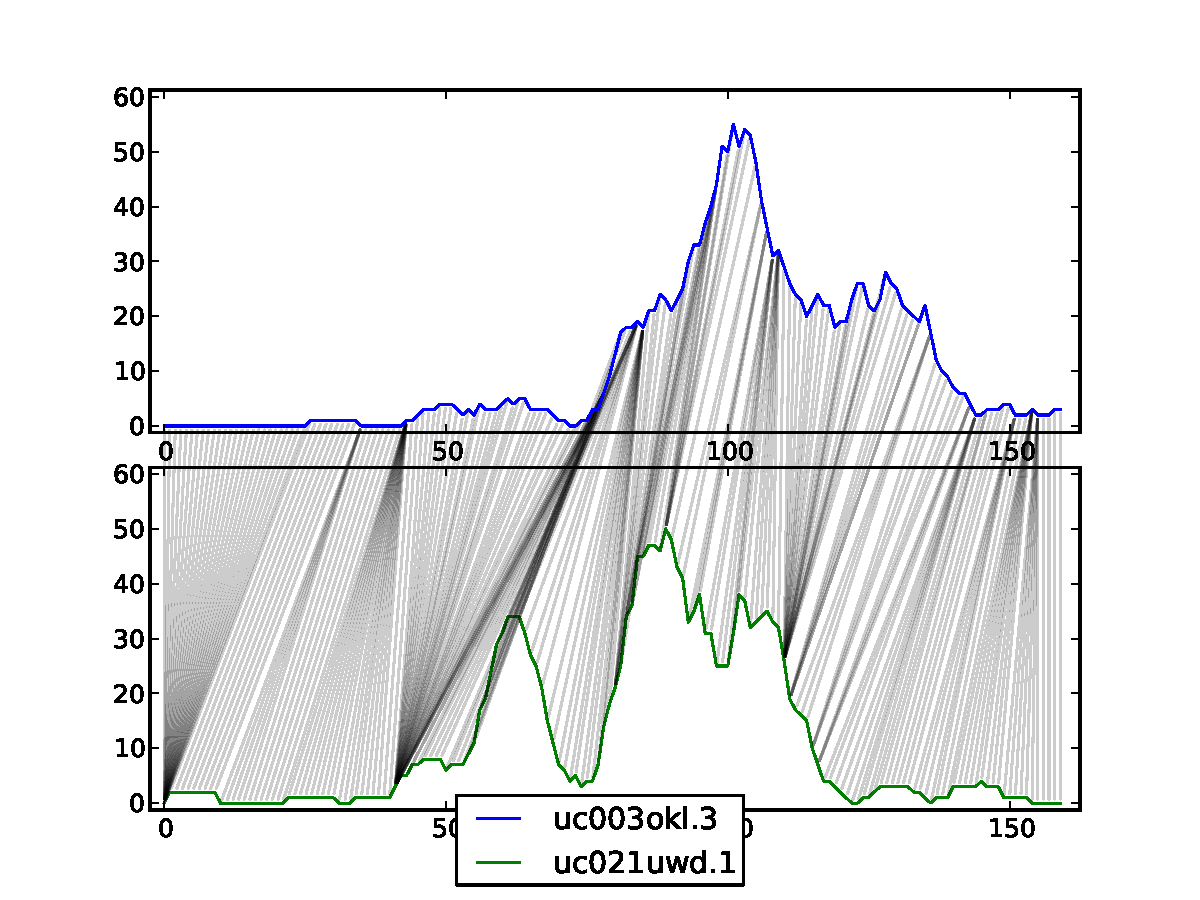
\includegraphics[width=\textwidth]{figures/DTW/uc003okl_3-uc021uwd_1-mappings-std.pdf}
       \caption{Alignments}
       \label{fig:DTW:std:mappings}
   \end{subfigure}
   ~
   \begin{subfigure}[b]{0.45\textwidth}
       \centering
       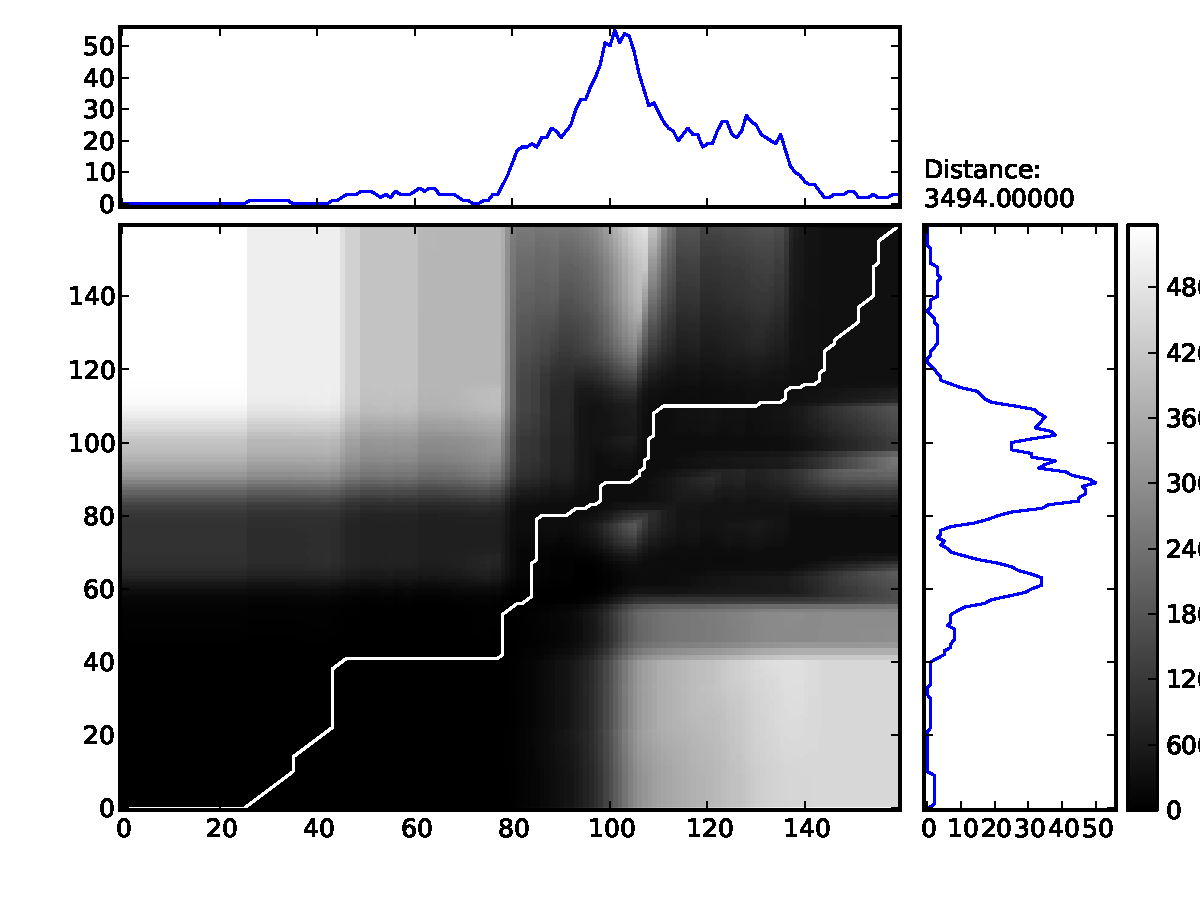
\includegraphics[width=\textwidth]{figures/DTW/uc003okl_3-uc021uwd_1-cost-std.pdf}
       \caption{Cost matrix and path}
       \label{fig:DTW:std:cost}
   \end{subfigure}
   \caption{Result of DTW distance calculation on the \histonemodification{H3K4Me3} Activation profiles around transcription start sites for two genes,  \gene{uc003okl.3} and \gene{uc021uwd.1}.}
   \label{fig:DTW:std}
\end{figure}

In some cases, warping the time axis arbitrarily might not necessarily be a correct thing to do.
For instance, have a look at \autoref{fig:DTW:std}. Here DTW is used to compare the \histonemodification{H3K4Me3} activation profiles around transcription start sites (TSS) of two genes, \gene{uc003okl.3} and \gene{uc021uwd.1}. We can immediately see that first activation profile appears to be unimodal, whereas the second one is clearly bimodal. The minimal warping path maps a relatively inactive region from around bin 40 to around bin 80 in the series for \gene{uc003okl.3} to a single point on the series for \gene{uc021uwd.1}. However, this unexpressed region might have biological significance, e.g. indicate removal of a nucleosome, and we might not want to allow it to be compressed to a single point. 

We can manually impose restrictions on warping paths that are allowed by introducing global constraints. Sakoe-Chiba Band is one of the most commonly used global constraints on DTW \citep{Ratanamahatana:2004wu}. 

\subsubsection{Sakoe-Chiba Band}

\begin{figure}
   \centering
   \begin{subfigure}[b]{0.45\textwidth}
       \centering
       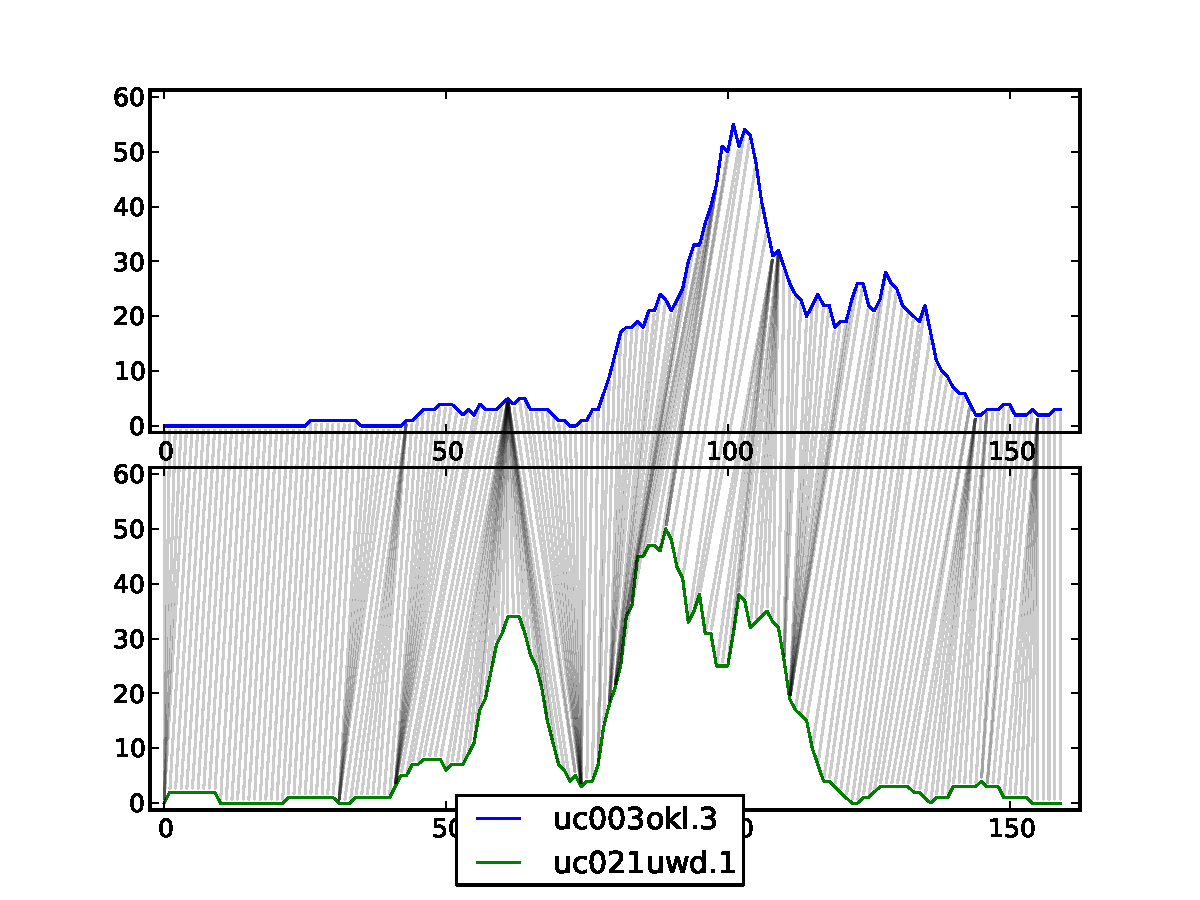
\includegraphics[width=\textwidth]{figures/DTW/uc003okl_3-uc021uwd_1-mappings-sakoe-chiba.pdf}
       \caption{Alignments}
       \label{fig:DTW:sakoe_chiba:mappings}
   \end{subfigure}
   ~
   \begin{subfigure}[b]{0.45\textwidth}
       \centering
       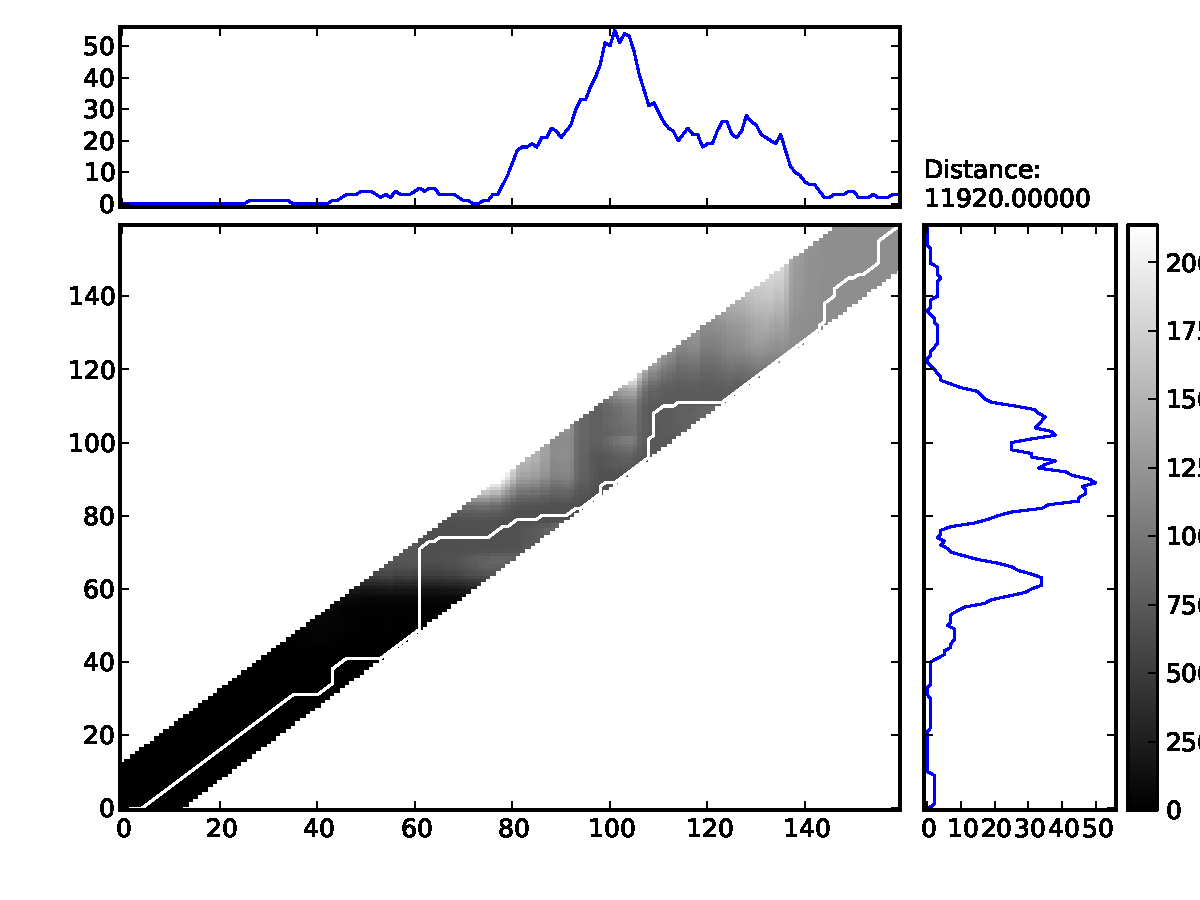
\includegraphics[width=\textwidth]{figures/DTW/uc003okl_3-uc021uwd_1-cost-sakoe-chiba.pdf}
       \caption{Cost matrix and path}
       \label{fig:DTW:sakoe_chiba:cost}
   \end{subfigure}
   \caption{Result of DTW distance calculation on the \histonemodification{H3K4Me3} Activation profiles around transcription start sites for two genes, \gene{uc003okl.3} and \gene{uc021uwd.1}. The DTW distance was constrained with Sakoe & Chiba constraint with $k = 12$.}
   \label{fig:DTW:sakoe_chiba}
\end{figure}

Sakoe \& Chiba constraint, as first described in \citep{Sakoe:1978ta} allows only the warping paths 
that satisfy $|i-j| \le k$ where $k$ is some integer specifying the tightness of the constraint. The constraint is commonly referred to as "Sakoe \& Chiba band" as the cost matrix has a shape of a band around the main diagonal (see \autoref{fig:DTW:sakoe_chiba:cost}). Such constraint reduces the complexity of DTW to $O(k \times max(n,m))$ where $n$ and $m$ are the lengths of the two sequences. 

Intuitively, the constraint requires that each point on sequence A is mapped to a point no more than $k$ points away on the sequence B. That is, it assumes that there won't be any warping of the time axis greater than by $k$ points. Note that setting the $k$ parameter to zero would give us Euclidean distance between the two sequences.

\autoref{fig:DTW:sakoe_chiba} compares the same regions in the \autoref{fig:DTW:std} using the DTW constrained with Sakoe \& Chiba band of length $k=12$. One can see that the peaks on the right-hand side of the two sequences are still aligned correctly, but the relatively inactive region in the first sequence is now forced to be mapped to the left peak in the second sequence, resulting in a huge cost penalty and making the sequences quite distant from each other. This alignment results in a total distance of 11920 using squared euclidean distance as the local distance measure. Compare that to the distance of 3494 obtained by unconstrained warping.

As far as the author is aware, there is no established way of picking the value of parameter $k$.
Historically, $k$ was set to 10\% of the length of the sequences.
For nearest-neighbour classification tasks, \cite{Ratanamahatana:2004wu} has shown that an even a window sufficiently smaller than 10\% gives the highest accuracy for some datasets, though the actual number strongly depends on the actual dataset. Due to this, the constraint $k$ is not imposed in the Dynamic Genome Warping package and is left as a free parameter the user could specify herself.

\subsubsection{Slanted Band Constraint}
\label{sec:slanted-band-constraint}

Sakoe \& Chiba band makes DTW incomputable for sequences whose lengths differ by more than $k$ items, as the last points of those sequences, point $n$ and point $m$, will not satisfy the constraint 
$|i-j| \le k$. The reason for this failure is the fact that $i=j$ is not the real diagonal of the cost matrix, if the lengths of the two sequences, $n$ and $m$, are not equal. 

Toni Giorgino \nocite{Giorgino:2009ue} was well aware of this problem when implementing the DTW module for R\footnote{The R Project For Statistical Computing - \url{http://www.r-project.org/}} where he included a modified version of Sakoe \& Chiba constraint, he calls a slanted band constraint \citep{Giorgino:2009ue}. 

Slanted band constraint solves the problem of different sequence lengths by changing the constraint to 
$|i - \frac{m}{n} \times j| <= k$, where $m$ and $n$ are the lengths of the two sequences being compared. This essentially changes the slope of the diagonal line to $\frac{m}{n}$ (cf. to slope being 1 in \citep{Sakoe:1978ta}).

Unfortunately, the meaning of the parameter $k$ is inconsistent in Giorgino's definition of the constraint. If the second sequence is longer than the first one, thus $m > n$, the constraint can be thought to scale the second sequence down to the length of the shorter sequence and then apply the Sakoe \& Chiba constraint of size $k$, meaning $k$ is in the units of the shorter sequence. However, if the second sequence is shorter than the first one, it will be essentially rescaled to match the length of the longer sequence and then the parameter $k$ will be measured in units of the longer sequence. In this particular case, DTW distance might not even be computable as in order for the warping path to remain continuous, for all $j$, there should be some $i$ within the allowed warping window, that is also either in the window of $j+1$ or is by at most one unit away from some $i'$ that is within the window of $j+1$. More formally, the following inequality must hold: 

\begin{equation}\label{eq:dtw:slanted-band:eq}
(j+1) \frac{m}{n} - k \le j \frac{m}{n} + k + 1
\end{equation}

After some algebraic calculations, inequality \ref{eq:dtw:slanted-band:eq} can be rewritten as:

\begin{equation}
\frac{m}{n} \le 2k + 1
\end{equation}

This inconsistency might not be important in the situations where we have a query sequence that we want to match to a reference sequence as the order of parameters will not change in these cases. However, symmetry is crucial for hierarchical clustering, therefore Giorgino's constraint was modified slightly to always assume that the first sequence is longer than the second one as described below.

The slope parameter is again calculated as $s = \frac{m}{n}$, however it is now always less than or equal to one. This slope is now applied to the first sequence, (not the second one as in \citep{Giorgino:2009ue}) essentially scaling it down to the length of the shorter sequence.
The new constraint is then formally defined as:
\begin{equation}
|\lceil i \times \frac{m}{n} \rceil - j| \le k
\end{equation}

Of course, there are no technical limitations preventing the slope to be applied on the second sequence as in the original paper \cite{Giorgino:2009ue}. The reason why this was changed and the slope applied on the first sequence is purely because the implementation is a bit more intuitive this way. 

This modified constraint is now always consistent, with the parameter $k$ always measured in units of the shorter sequence.

\subsubsection{Correction for Antisense Regions}
\begin{figure}
    \centering
    \begin{subfigure}[b]{0.3\textwidth}
         \centering
         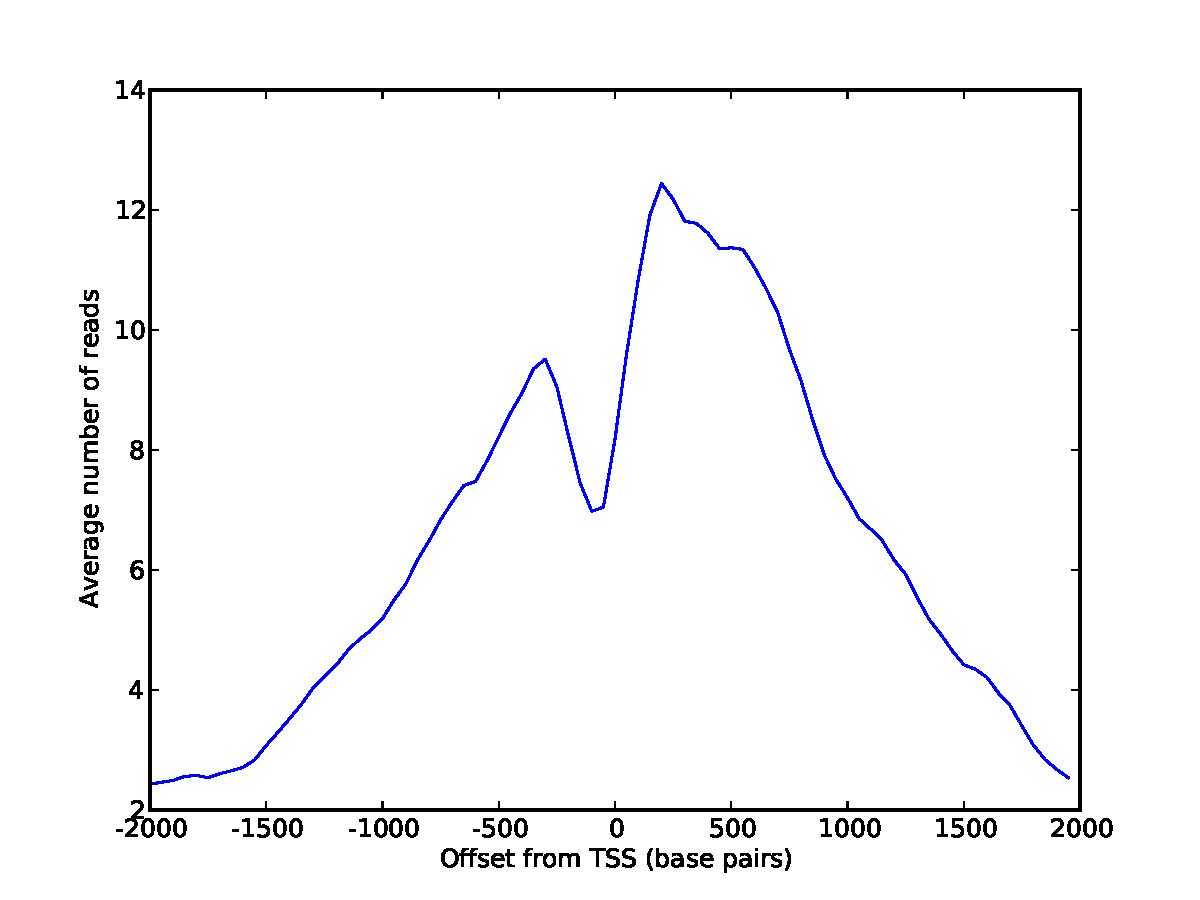
\includegraphics[width=\textwidth]{figures/DTW/forward_strand.pdf}
         \caption{Forward strand}
         \label{fig:DTW:antisense_comparison:forward}
    \end{subfigure}
    ~
    \begin{subfigure}[b]{0.3\textwidth}
         \centering
         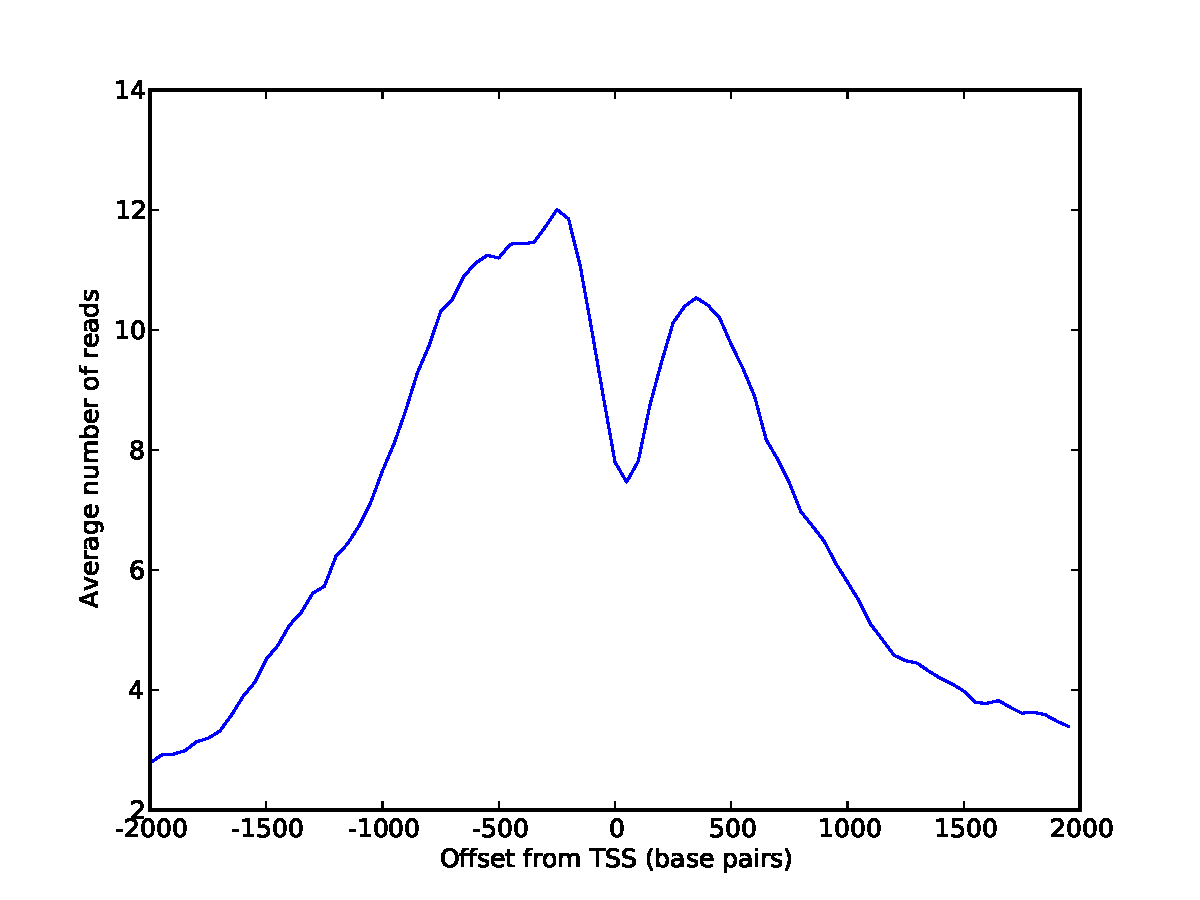
\includegraphics[width=\textwidth]{figures/DTW/reverse_strand.pdf}
         \caption{Reverse strand}
         \label{fig:DTW:antisense_comparison:reverse}
    \end{subfigure}
    \caption{\histonemodification{H3K4Me3} profiles for regions around transcription start sites within ENCODE pilot regions \cite{ENCODEProjectConsortium:2007fu}. Genes known to be transcribed on the forward strand are pictured in (a), whereas genes known to be transcribed on the reverse strand are pictured in (b). Note the symmetry between these marks.}
    \label{fig:DTW:antisense_comparison}
\end{figure}

\autoref{fig:DTW:antisense_comparison} shows the average profiles of regions around annotated transcription start sites in the ENCODE pilot regions of the genome \cite{ENCODEProjectConsortium:2007fu}. The average patterns are evidently symmetrical along the horizontal axis.
Even though this directionality is generally known for patterns around well-annotated regions, such as the transcription start sites, the directionality for other regions of interest, such as peaks found by a peak caller, is rarely known.  

In order to be able to account for this opposing directionality, every DTW comparison that is made when clustering, is actually made twice: once as described in previous sections, and once with one of the patterns reversed. The smaller distance between the two is then returned as the true distance between the patterns. 

Of course, DGW also supports an option to turn this behaviour off, in case we would like to force the different strands into different clusters, or an option to use the annotated strandedness, if it is provided.

\subsection{DTW Projection}
\label{sec:dtw-projection}

Just like one can project a vector in euclidean space onto a new basis, one can project some time series onto the time axis of another time series with the help of DTW. 

Given the original sequence $\mathbf{a}$, the basis sequence $\mathbf{b}$, and the warping path between the two sequences, $p$, we can project $\mathbf{a}$ onto $\mathbf{b}$ by computing the average value of all points mapped to every point of sequence $\mathbf{b}$.

More formally, each point $x_k$ of the projected sequence is computed by the following equation:
\begin{equation}
    x_k =  \frac{\sum_{(i,j) \in p} a_i \times \delta_{j=k}}{\sum_{(i,j) \in p} \delta_{j=k}} 
\end{equation}

Where $k=1..|\mathbf{b}|$ and $\delta_{j=k}$ is the delta function that is $1$ when $j=k$, and $0$ otherwise.\todo{Put a worked example here as well}

\begin{figure}[t,b]
   \centering
   \begin{subfigure}[b]{0.31\textwidth}
       \centering
       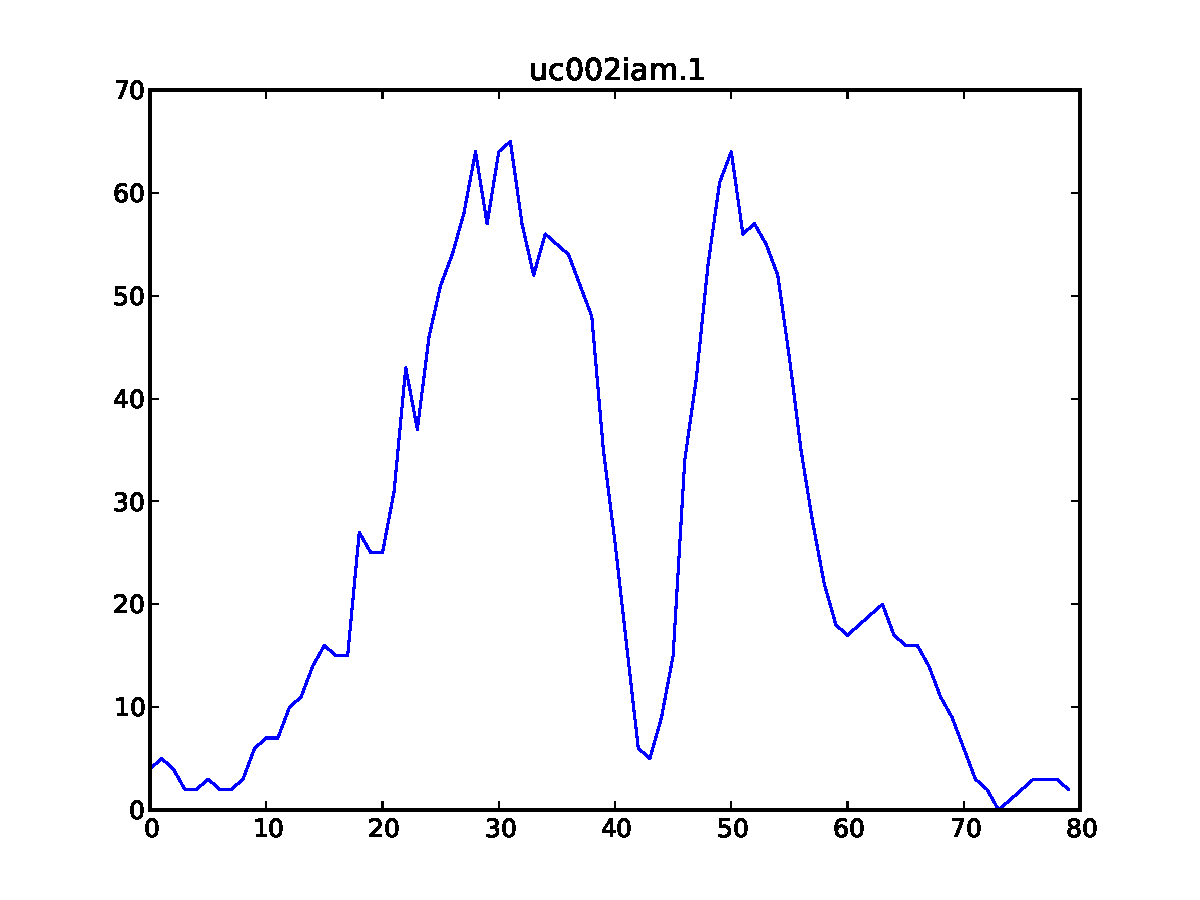
\includegraphics[width=\textwidth]{figures/DTW/sequence.pdf}
       \caption{Sequence}
       \label{fig:DTW:projection:sequence}
   \end{subfigure}
   ~
   \begin{subfigure}[b]{0.31\textwidth}
       \centering
       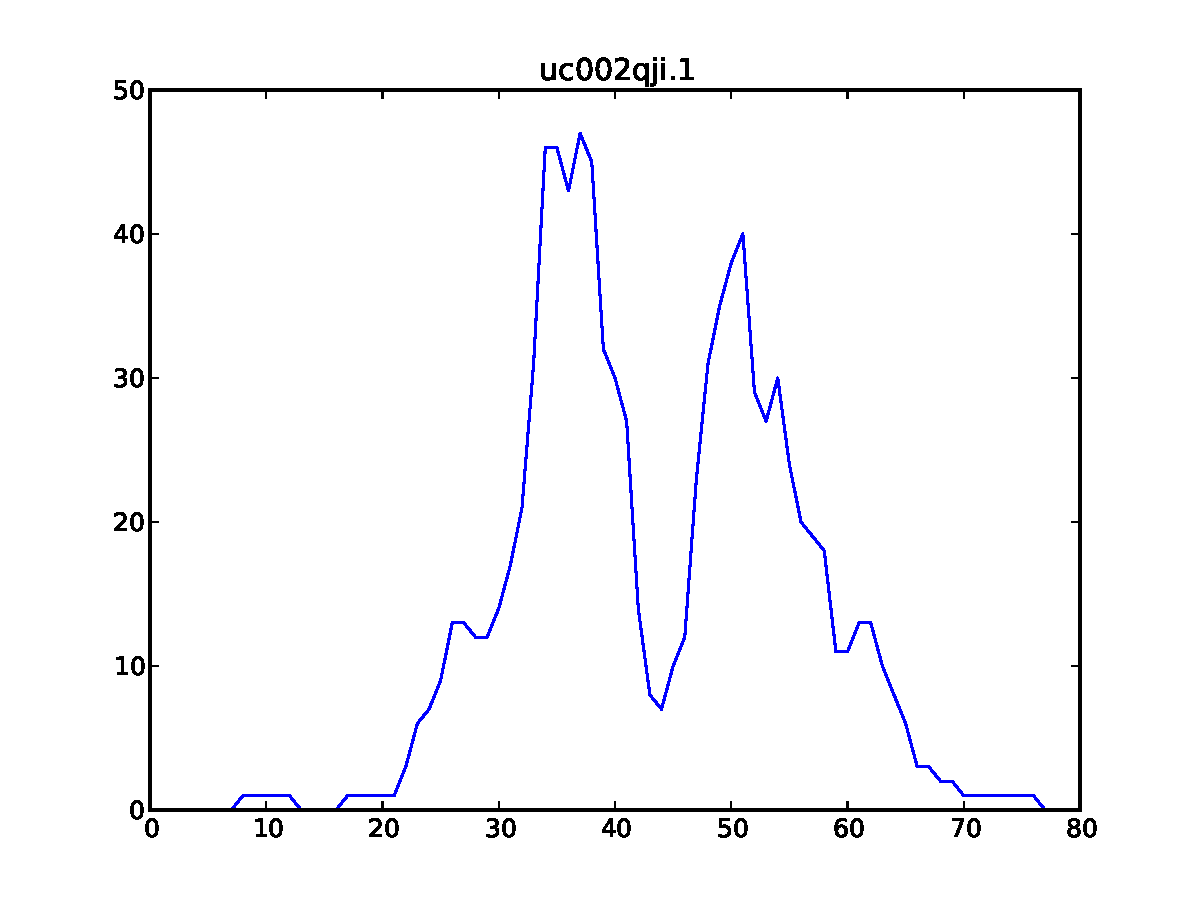
\includegraphics[width=\textwidth]{figures/DTW/basis.pdf}
       \caption{Basis}
       \label{fig:DTW:projection:basis}
   \end{subfigure}
   ~
   \begin{subfigure}[b]{0.31\textwidth}
       \centering
       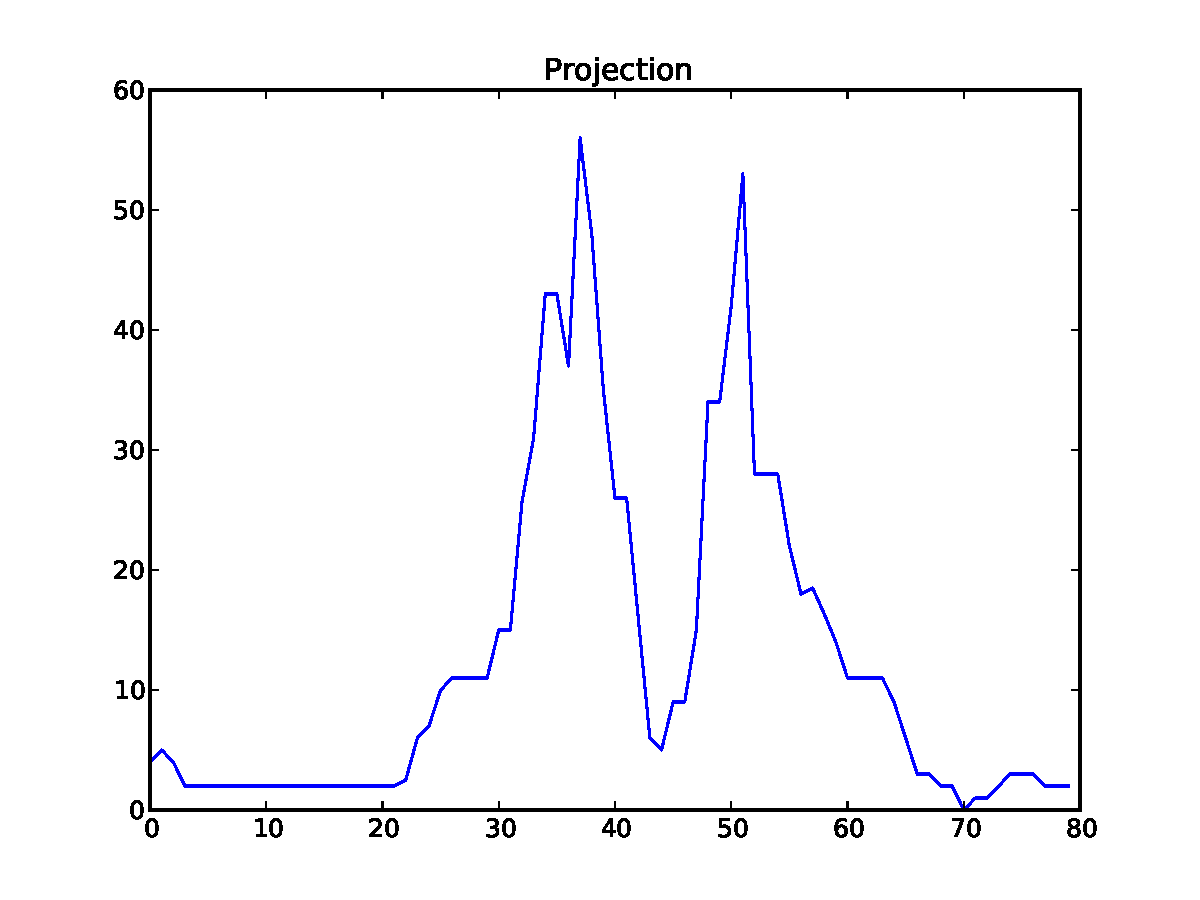
\includegraphics[width=\textwidth]{figures/DTW/projection.pdf}
       \caption{Projection}
       \label{fig:DTW:projection:projection}
   \end{subfigure}
   \caption{Result of projecting sequence, pictured in \ref{fig:DTW:projection:sequence} onto the basis, pictured in \ref{fig:DTW:projection:basis} with unconstrained DTW used to generate the warping path.}
   \label{fig:DTW:projection}
\end{figure}

\autoref{fig:DTW:projection} illustrates the result of projecting one histone mark around the transcription start site onto another.

\section{Clustering}
\label{sec:clustering}

Previous chapters have defined the mechanics of DTW distance. The important question that is yet to be raised is how the data can be clustered under it. 

It has been shown, that under the DTW distance, computation of a sequence that minimises the distance to all other sequences in the cluster, so called centroid sequence, is a NP-Complete problem as the search space grows exponentially with number of sequences being averaged \cite{Hautamaki:2008fh,Petitjean:2012bp}.

Even though a variety of methods to approximate this calculation have been proposed through the years, \cite{Gupta:1996tw,Niennattrakul:2009ep,Petitjean:2011bq,Petitjean:2012bp}, one needs to be careful before using any of them for clustering, because incorrect averaging methods might create incorrect clusterings, e.g. allow the averaged center drift outside the sequences being averaged \cite{Niennattrakul:2007wv}. Due to this, implementation of centroid-based clustering methods (e.g. k-means) under Dynamic Time Warping distance is usually tricky.

Hierarchical-clustering methods, on the other hand, do not require a notion of centroid. One of the hierarchical clustering methods, agglomerative clustering, works by first computing the distances between all pairs of points in the dataset, then joining the two closest points into a cluster, forming a new cluster this way. Then the second two closest points are joined forming yet another cluster, and so on, eventually joining all of the points. 

The comparison between two clusters is usually done in one of the following ways:

\begin{itemize}
   \item \emph{Single linkage:} The distance between two clusters is equal to the smallest distance between the any two elements in the two clusters.
   \item \emph{Complete linkage:} The distance between two clusters is equal to the largest distance between any two elements in the two clusters.
   \item \emph{Average linkage:} The distance between two clusters is equal to the average of the distances between the elements in the clusters.
\end{itemize}
\todo{Visualise this}

\begin{figure}
    \centering
    \begin{subfigure}[b]{0.45\textwidth}
        \centering
        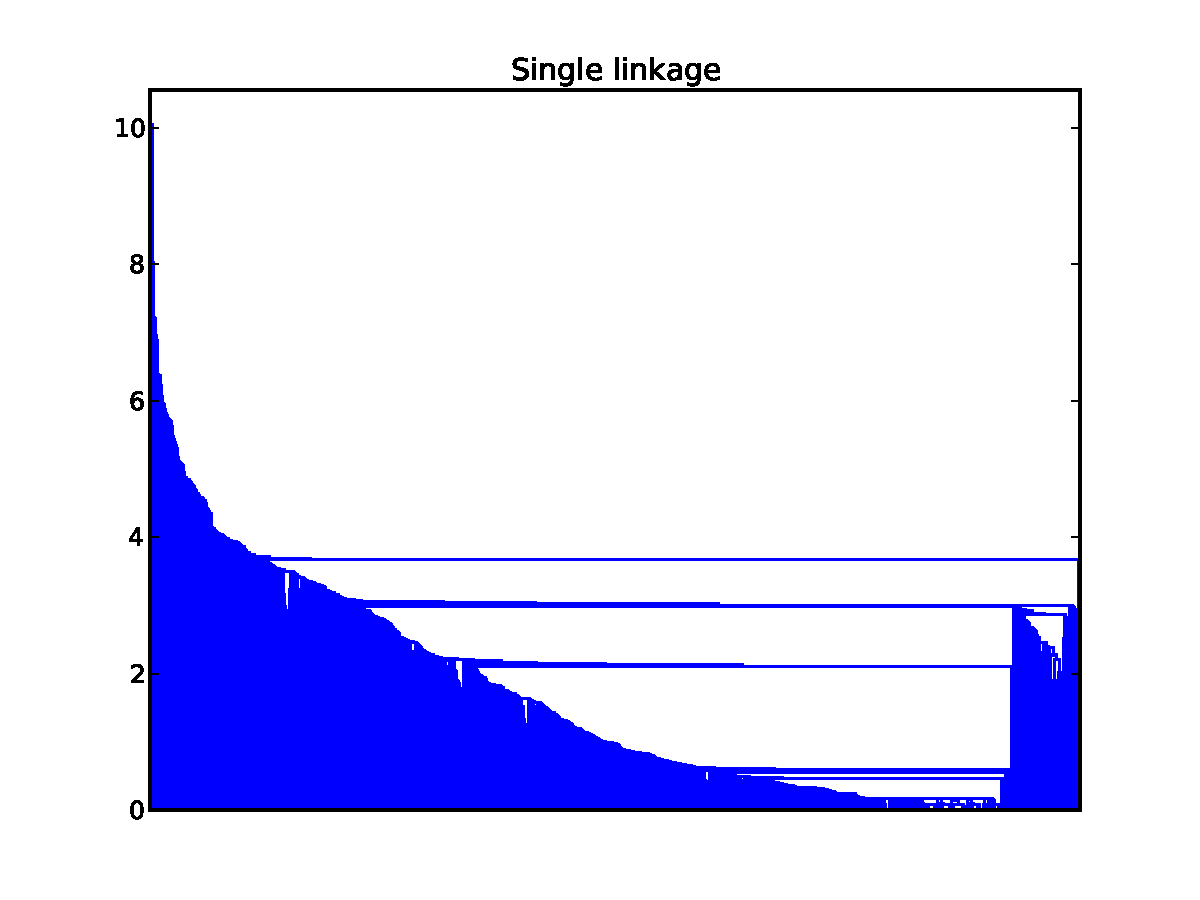
\includegraphics[width=\textwidth]{figures/clustering/linkage_single.pdf}
        \caption{Single linkage}
        \label{fig:clustering:dendrogram:single}
    \end{subfigure}
    ~
    \begin{subfigure}[b]{0.45\textwidth}
        \centering
        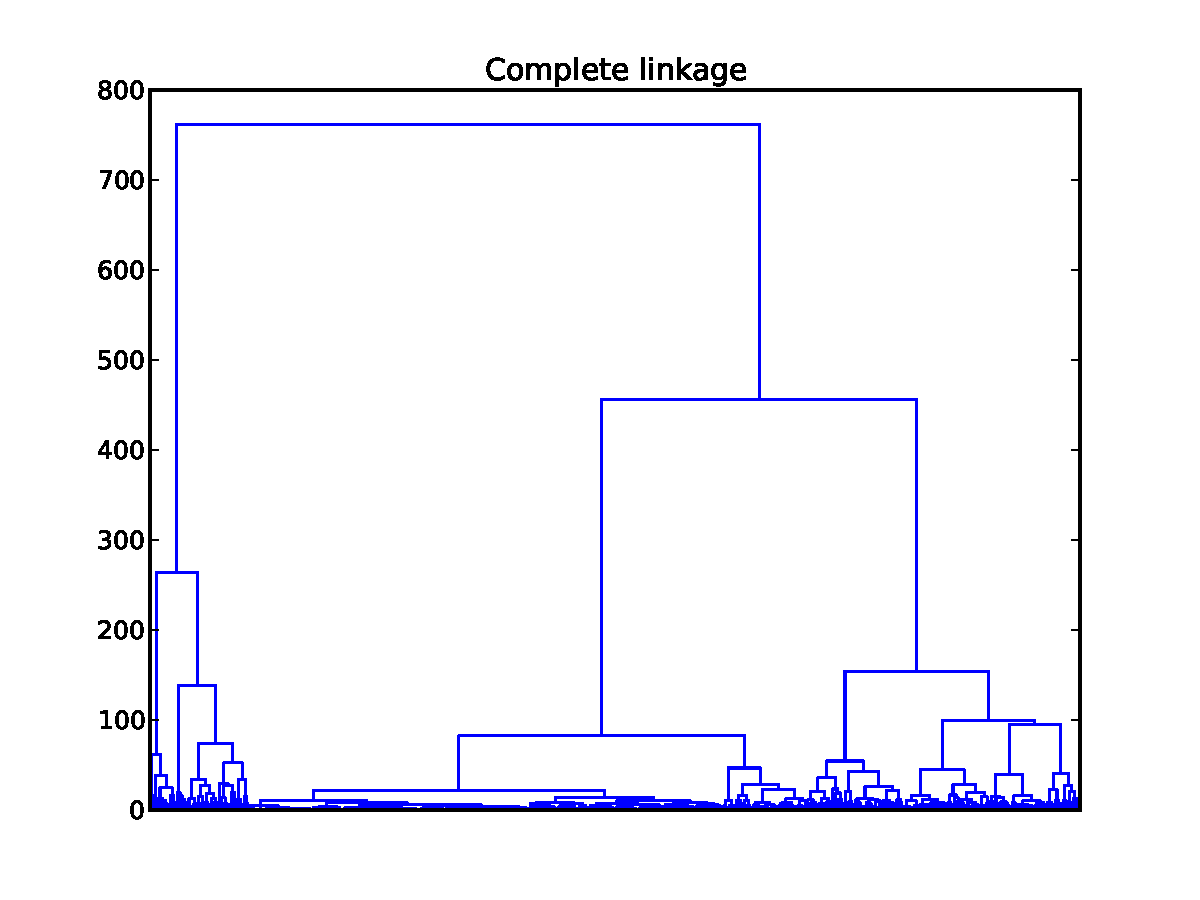
\includegraphics[width=\textwidth]{figures/clustering/linkage_complete.pdf}
        \caption{Complete linkage}
        \label{fig:clustering:dendrogram:complete}
    \end{subfigure}
    \caption{Comparison of dendrograms obtained by clustering using single and complete linkages. The datasets being clustered are the same, generated from \celltype{K562} \histonemodification{H3K4Me3} dataset, and unconstrained DTW distance metric was used to cluster both of them. The only thing that is different is the linkage method.
      One can see chaining of the items in the single linkage clustering  dendrogram (\ref{fig:clustering:dendrogram:single}), where each element is subsequently added to the same cluster, rather than forming many smaller clusters before, when complete linkage is used (\ref{fig:clustering:dendrogram:complete}).}
    \label{fig:clustering:dendrogram}
\end{figure}

Agglomerative clusterings that use single linkage criterion are vulnerable to the phenomenon known as \emph{chaining}. This phenomenon occurs, when instead of forming distinct clusters early, agglomerative clustering algorithm forms a single cluster and incrementally joins more and more elements to it, one at the time. This is illustrated in \autoref{fig:clustering:dendrogram:single}. 
Here it seems that majority of data is in one cluster and each data point is joined to the cluster one by one, creating a smooth downwards facing slope seen in the figure. 

This is by no means a meaningful clustering, as 
if we were to cut the dendrogram at pretty much any threshold we would get the majority of the data in one of the clusters, with the remaining data points having a separate cluster for themselves. 

We can see that chaining behaviour is not visible when complete linkage is used. Here, the clusters are formed early, and then joined later on, as one would expect (\autoref{fig:clustering:dendrogram:complete}). In fact, Hirano et al. \cite{Hirano:2005wh} have shown empirically that out of the three linkage methods discussed above, only complete linkage was able to produce meaningful clusters when clustering time series data under DTW. Due to this reason, DGW computes the distances between two clusters using complete linkage criterion.

\subsection{Forming Flat Clusters}

It is also worth noting, that there have been attempts to relax the requirement of having a notion of centroid in centroid clustering methods by using a medoid -- a representative object from within the cluster. For instance, k-medoids algorithm, implemented e.g. in \cite{Park:2009ks}, could in theory be used to cluster DTW distances. 

The disadvantage of this method against hierarchical clustering is the fact that the number of clusters, the $k$ in k-medoids, needs to be picked before the clustering was done. Several iterations of the algorithm could be run, and the results with different $k$s could be compared, of course, yet it is both not efficient to do, and not clear what metric should be used to
measure the meaningfulness of the clustering in this case.

Hierarchical clustering methods, on the other hand, do not need the number of clusters decided beforehand, as the number of flat clusters can be chosen \emph{after} the clustering was done. This
allows inspection of the clustering results to guide this process.

This cutting can either be done automatically, if there is clear way to do this, e.g. if the distances in the dendrogram correspond to p-values, like in \cite{Wang:2012cb}, or by simple visual inspection of the resulting dendrogram. The latter approach is implemented in this project.

\subsection{Cluster Prototypes}
\label{sec:prototypes}

After the flat clusters are formed, the clusters need to be visualised to the user somehow. Just displaying the original data (i.e. in the form of a heatmap) is insufficient, as such representation of the data does not does not explain why the data was clustered together in the first place. 

The end user of the software, would want to see the data represented after warping, i.e. average profile of the warped data, as to be able to get the structure and the shape of the resulting cluster marks. The problem of extracting this average warped profile lies in the fact that only two sequences are compared with each other at the time, and both of them can be arbitrarily warped. What this means, unfortunately, that the same sequence might be warped in as many ways as there are sequences to compare it against. In order to be able to give an average warping of sequences in a cluster, one needs to agree upon the base sequence upon which to warp the remaining sequences on. In other words,
one needs to find a prototype for the cluster in order to be able to visualise the warped items. Once this prototype sequence is chosen, DTW projection (\autoref{sec:dtw-projection}) can be used to warp the original data onto the basis defined by the prototype.

Remember that inability to compute perfect centroids was one of the reasons why hierarchical clustering was chosen in favour of centroid-clustering in the first place. Then we were worried about the bias in the data clustering producing clusters that are not meaningful. However, at this case the data is already clustered and flat clusters are already formed. Some prototyping error is tolerable here as it won't be able to accumulate as easily as it would during clusteirng. The only requirement that is posed on the prototype is that it expresses a similar shape than the marks being clustered visually.


\subsubsection{Prioritised Shape Averaging}
A method called Prioritised Shape Averaging (PSA), proposed in \cite{Niennattrakul:2009ep}, was chosen to generate the cluster prototypes. The reason why PSA was chosen, in favour of other methods, is the fact that it can exploit the hierarchical structure, we've already computed in prototype generation stage.

The basic idea under the PSA can be thought of in terms of bottom-up algorithm.
Initially, make all of the leaf nodes to be the prototypes of themselves, with the weight of one assigned to each of them. Moving up the clustering tree, for each node, average the two prototypes of the left and right child of the node (remember that hierarchical clustering trees are always binary), with some averaging procedure that takes the weights of the two nodes into account. Make the weight of this newly formed node equal to the number of elements in that node.

The proposed method to be used in PSA is Scaled Dynamic Time Warping (SDTW) averaging algorithm that is also defined in the paper. This algorithm works similarly to the standard path averaging algorithm, which is defined as follows: For each pair of points on the DTW warping path, $(i,j)$, average the corresponding points in the two sequences $a_i$, and $b_j$, in the following way:
\begin{equation} \label{eq:standard_path_averaging}
 x =  \frac{\lambda_a \times a_i + \lambda_b \times b_j}{\lambda_a + \lambda_b}
\end{equation}

Essentially, it is doing weighted averaging of these paths.
SDTW extends this definition, by making the algorithm "stretch" the resulting point $x$,  $\lambda_a$ times, if the point in sequence $\mathbf{a}$ was unchanged compared to previous pair of points in the path, i.e. the warping path moved straight upwards; $\lambda_b$ times if the warping path moved horizontally, $\frac{\lambda_a + \lambda_b}{2}$ times if the warping path moved diagonally.

Now it is obvious to see how such averaging method would create paths that are getting longer and longer as more and more points are being averaged. The proposed solution for this problem is to rescale the resulting average path to be of the length of one of the two sequences. As a convention, I always use the length of the longer sequence when rescaling the path.

\begin{figure}
    \centering
    \begin{subfigure}[b]{0.45\textwidth}
        \centering
        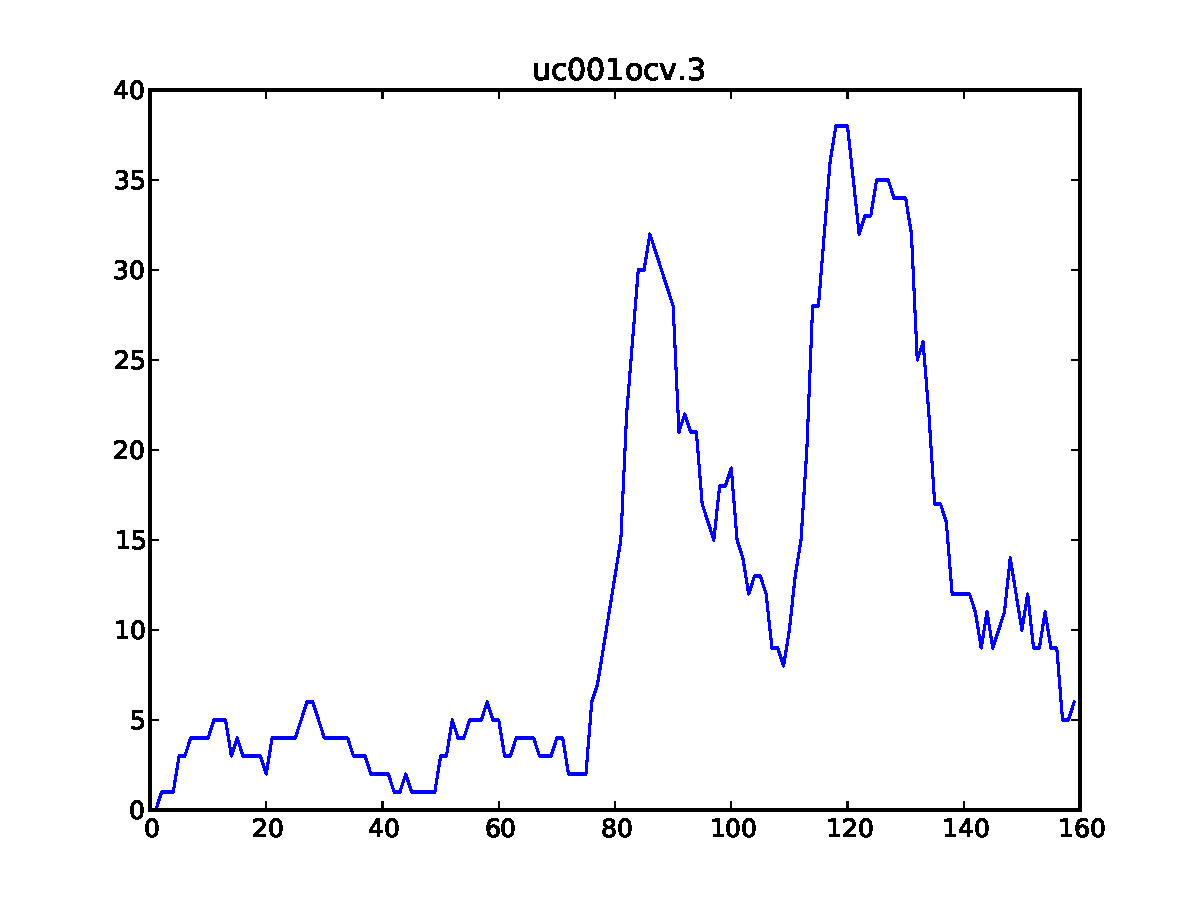
\includegraphics[width=\textwidth]{figures/clustering/prototypes/uc001ocv_3.pdf}
        \caption{Sequence A, weight 10}
        \label{fig:clustering:prototypes:seq_a} 
    \end{subfigure}
    ~
    \begin{subfigure}[b]{0.45\textwidth}
        \centering
        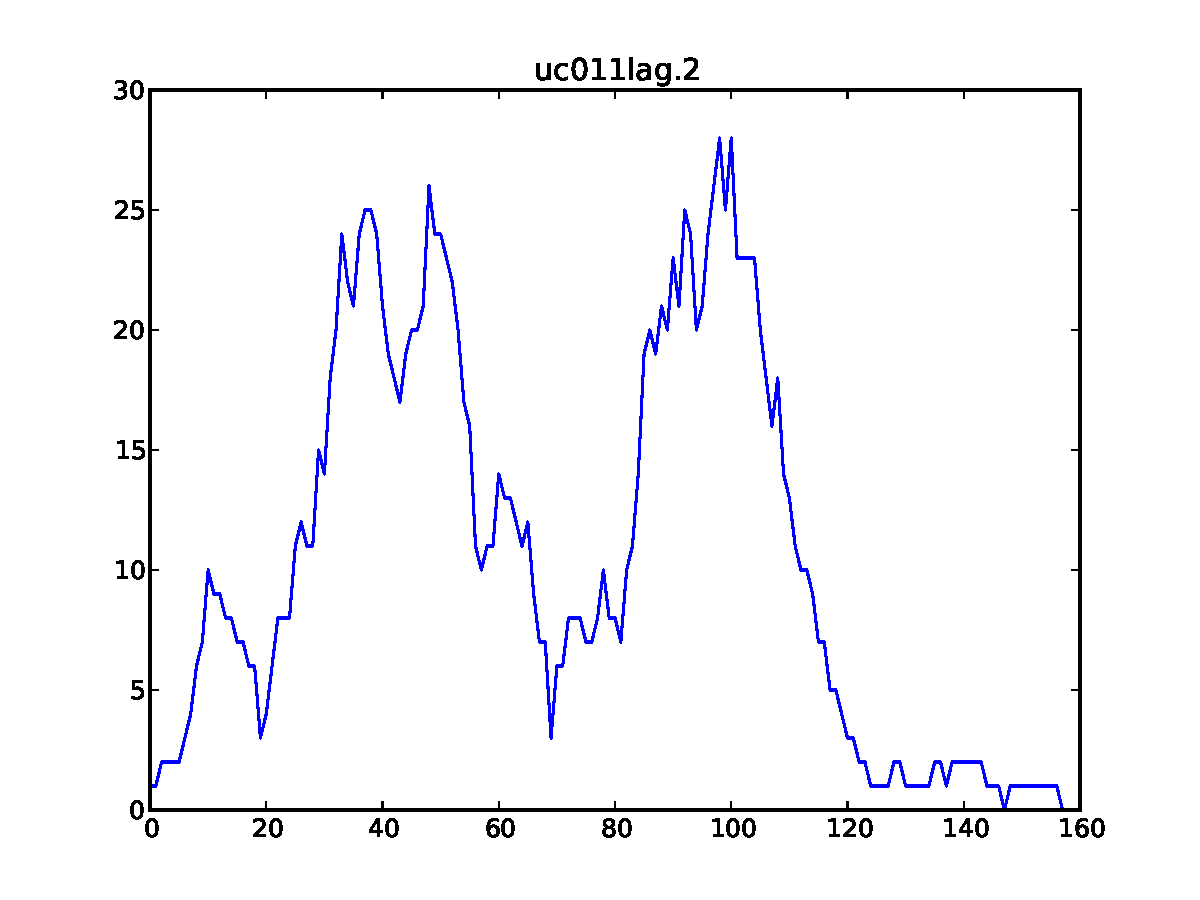
\includegraphics[width=\textwidth]{figures/clustering/prototypes/uc011lag_2.pdf}
        \caption{Sequence B, weight 50}
        \label{fig:clustering:prototypes:seq_b} 
    \end{subfigure}
    ~
    \begin{subfigure}[b]{0.31\textwidth}
        \centering
        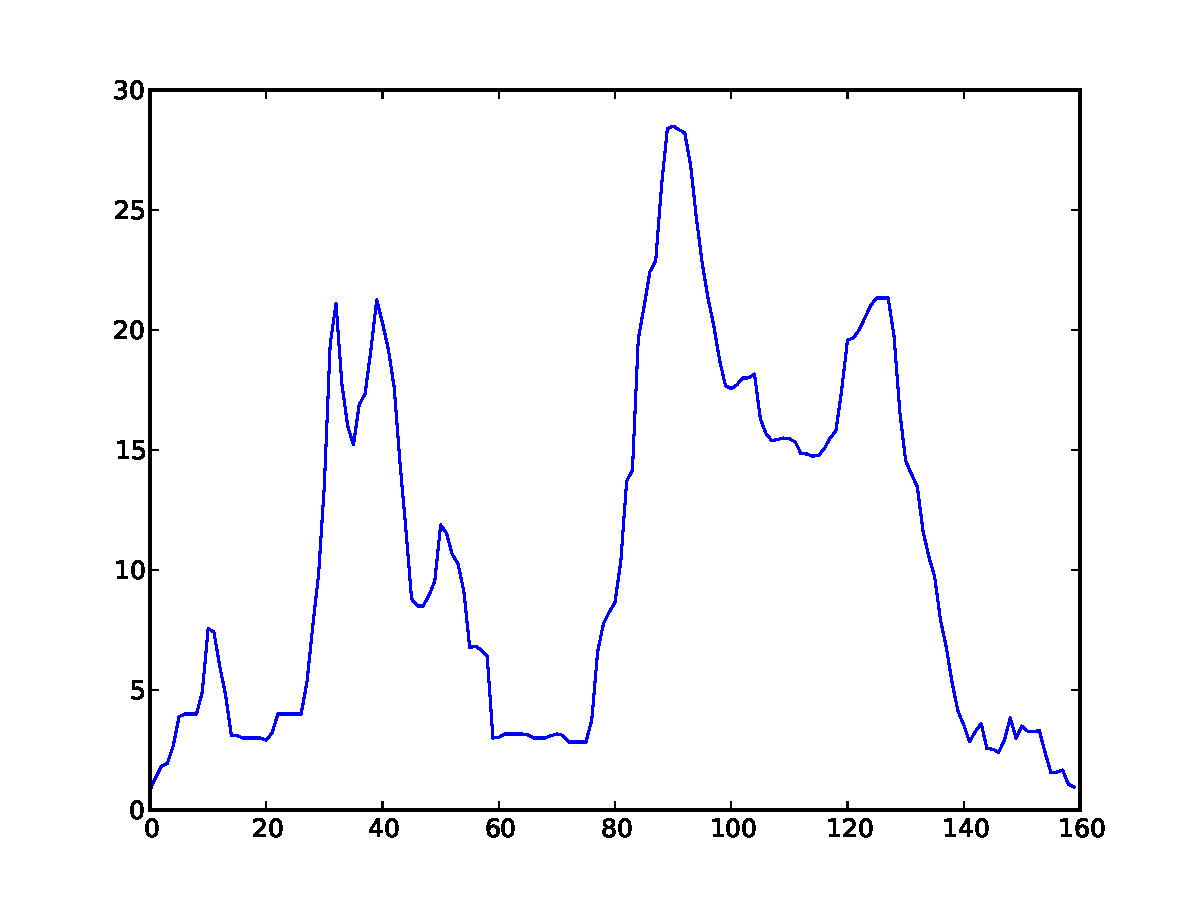
\includegraphics[width=\textwidth]{figures/clustering/prototypes/psa.pdf}
        \caption{SDTW}
        \label{fig:clustering:prototypes:sdtw}
    \end{subfigure}
    ~
    \begin{subfigure}[b]{0.31\textwidth}
        \centering
        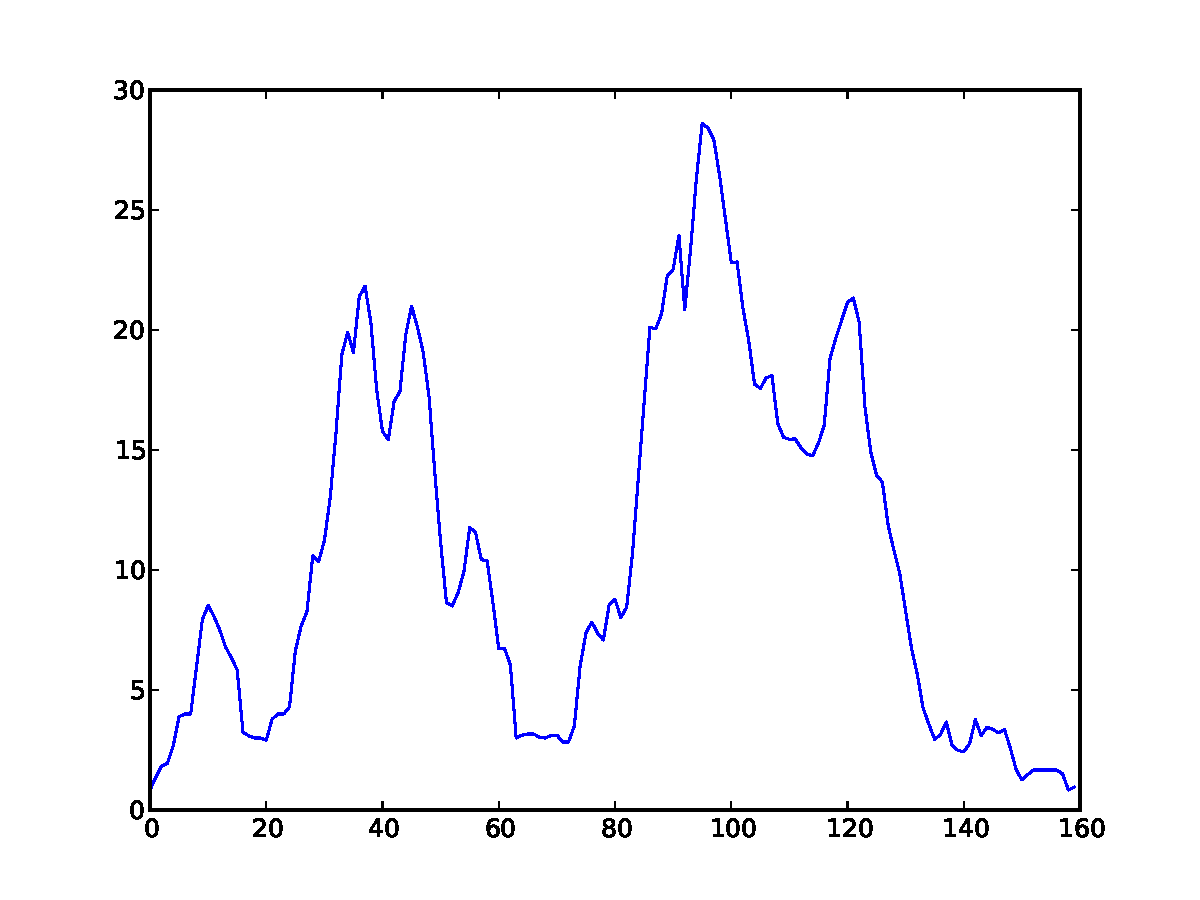
\includegraphics[width=\textwidth]{figures/clustering/prototypes/std.pdf}
        \caption{Standard}
        \label{fig:clustering:prototypes:std}
    \end{subfigure}
    ~
    \begin{subfigure}[b]{0.31\textwidth}
        \centering
        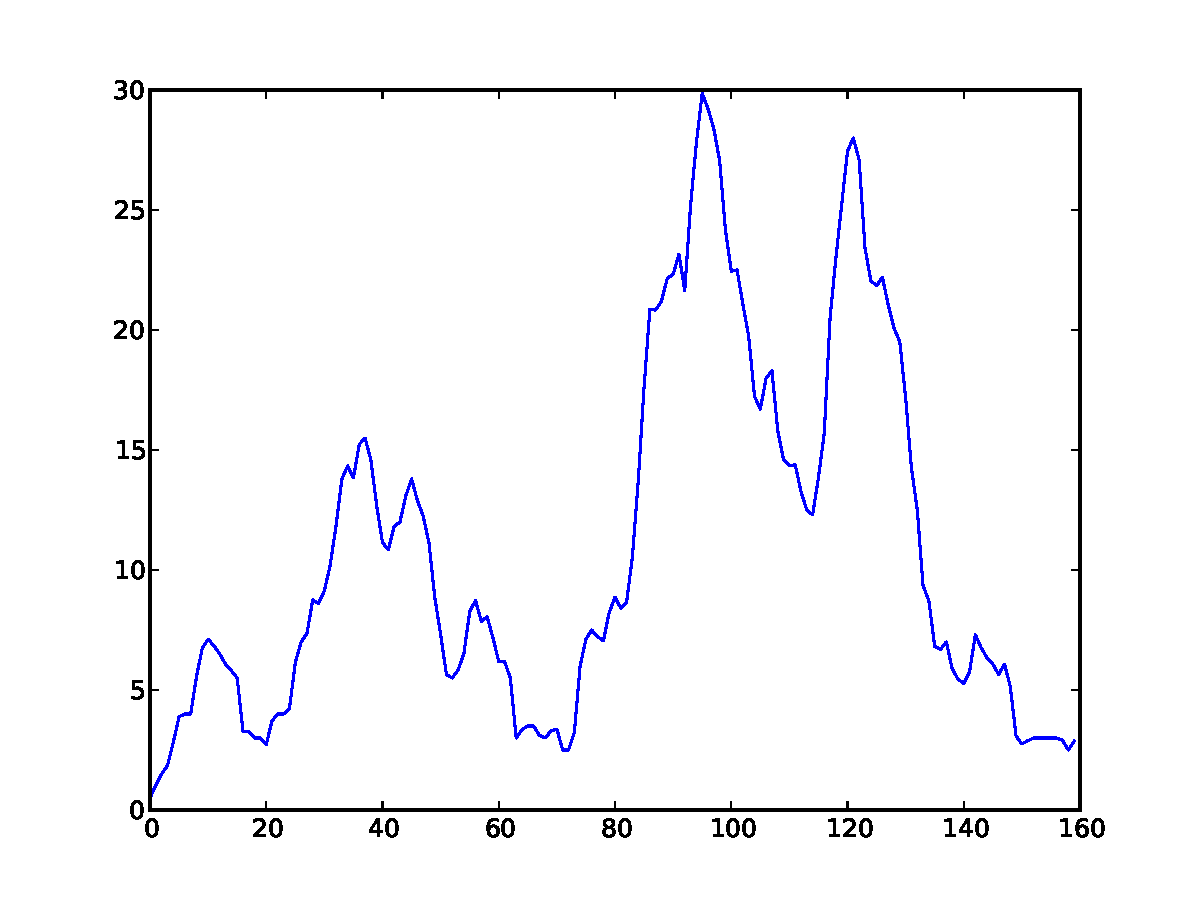
\includegraphics[width=\textwidth]{figures/clustering/prototypes/unweighted.pdf}
        \caption{Standard-Unweighted}
        \label{fig:clustering:prototypes:unweighted}
    \end{subfigure}
    \caption{Visualisation of the three prototyping methods discussed in \autoref{sec:prototypes}. Two sequences in \ref{fig:clustering:prototypes:seq_a} and \ref{fig:clustering:prototypes:seq_b} were averaged with each other using DTW with Sakoe & Chiba band constraint set to 12. The first sequence had a weight of 10, whereas the second sequence had a weight of 50. The results using various averaging methods are shown in \ref{fig:clustering:prototypes:sdtw}, \ref{fig:clustering:prototypes:std} and \ref{fig:clustering:prototypes:unweighted}.}
    \label{fig:clustering:prototypes}
\end{figure}

\autoref{fig:clustering:prototypes} compares the STDW averaging method with standard averaging method as in \autoref{eq:standard_path_averaging} as well as to standard unweighted averaging method (where $\lambda_a = \lambda_b = 1$). One can see that the average sequences produced by both SDTW and standard averaging methods favour the sequence with more weight strongly and therefore resulting average does resemble the second sequence more than the first one. Compare this to unweighted average of the two sequences, where the new shape resemble both features equally. 

From these figures, it is hard to spot the difference between prototypes generated by SDTW and Standard methods in this particular case. Surprisingly, I did not find any but miniscule improvements SDTW makes to the end result of cluster prototype along the whole hierarchical clustering tree. These improvements seem not worth the extra overhead incurred by the clever treatment of these path changes, and therefore the DGW uses standard path averaging by default (though the user is able to override this, if she wants to).

\section{Reading and Preprocessing Data}
\label{sec:reading_and_preprocessing}

\begin{figure}
   \centering
   \copyrightbox{
   \begin{subfigure}[b]{0.3\textwidth}
       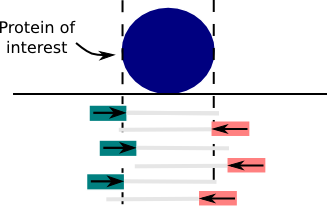
\includegraphics[width=\textwidth]{figures/methods/reading/read-shift.png}
       \caption{}
       \label{fig:methods:reading:shifts:broken}
   \end{subfigure}
   ~
   \begin{subfigure}[b]{0.3\textwidth}
       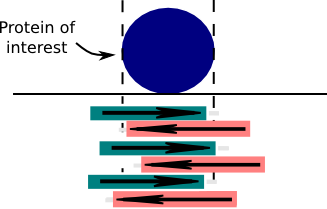
\includegraphics[width=\textwidth]{figures/methods/reading/read-shift-extended.png}
       \caption{}
       \label{fig:methods:reading:shifts:fixed}
   \end{subfigure}
   }
   {Inspired by a similar figure in \cite{Park:2009wc}.} 
   \caption{Illustration of the reasoning for extending the ChIP-Seq aligned reads. The DNA attached to the protein is pictured in grey, while the sequenced reads are pictured as coloured rectangles. In general, these short sequenced reads will not capture the true structure of the DNA that is bound to protein, as seen in (a). This can be mitigated by extending these reads to some length after the alignment, as shown in (b).}
    \label{fig:methods:reading:shifts}
\end{figure}


As previously mentioned in \autoref{sec:chip}, the result of ChIP-Seq experiment is a collection of short reads that are aligned to the reference genome, as pictured in \autoref{fig:background:chip-results}. In order to compute the activation profiles, each of the regions of interest are split into a series of bins of equal width. This bin width is simply referred to as \emph{read resolution}. The number of reads that falling within these bins is then counted to produce the activation mark.

Of course, as the reader might remember, usually only a short fragment of the DNA attached to the target protein is sequenced. In some cases, these short reads will not be able to capture the true distribution of DNA attached to the target proteins, as pictured in \autoref{fig:methods:reading:shifts:broken}. In order to mitigate this problem, DGW extends all reads to be 200 base pairs wide as pictured in \autoref{fig:methods:reading:shifts:fixed}.

\subsection{Highest Pileup Filter}
Intuitively, the less reads collect to the same bin, the more likely this could have happened due to one kind of noise or another. Given a long-enough region, even in a setting where reads arrive to bins completely at random, there will be at least a few bins within that region that will have at least a few reads piled up. Even though these regions provide little meaning biologically, they still need the same amount of CPU operations to be processed as every other region. With this in mind, DGW employs a filtering strategy that automatically filters regions that do not have a single bin with more than 10 reads piled up inside. Again, as with other parameters this number can be easily changed by the user.

\subsection{Pileup Height Normalisation}
\label{sec:pileup_height_normalisation}
\begin{figure}
   \centering
   \begin{subfigure}[b]{0.3\textwidth}
       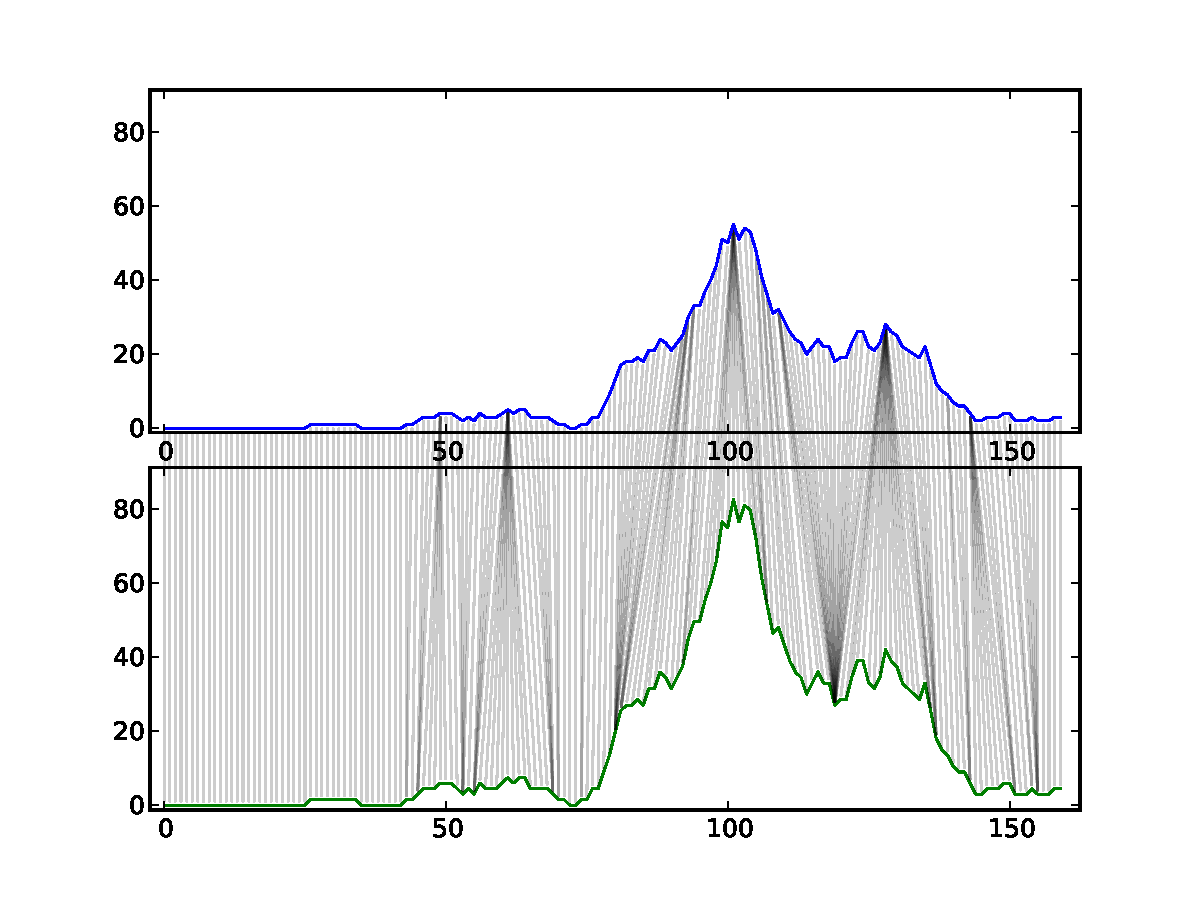
\includegraphics[width=\textwidth]{figures/methods/pileup_normalisation/mappings_x_1_5_x.pdf}
       \caption{}
       \label{fig:pileup_normalisation:mappings_unnormalised}
   \end{subfigure}
   ~
   \begin{subfigure}[b]{0.3\textwidth}
       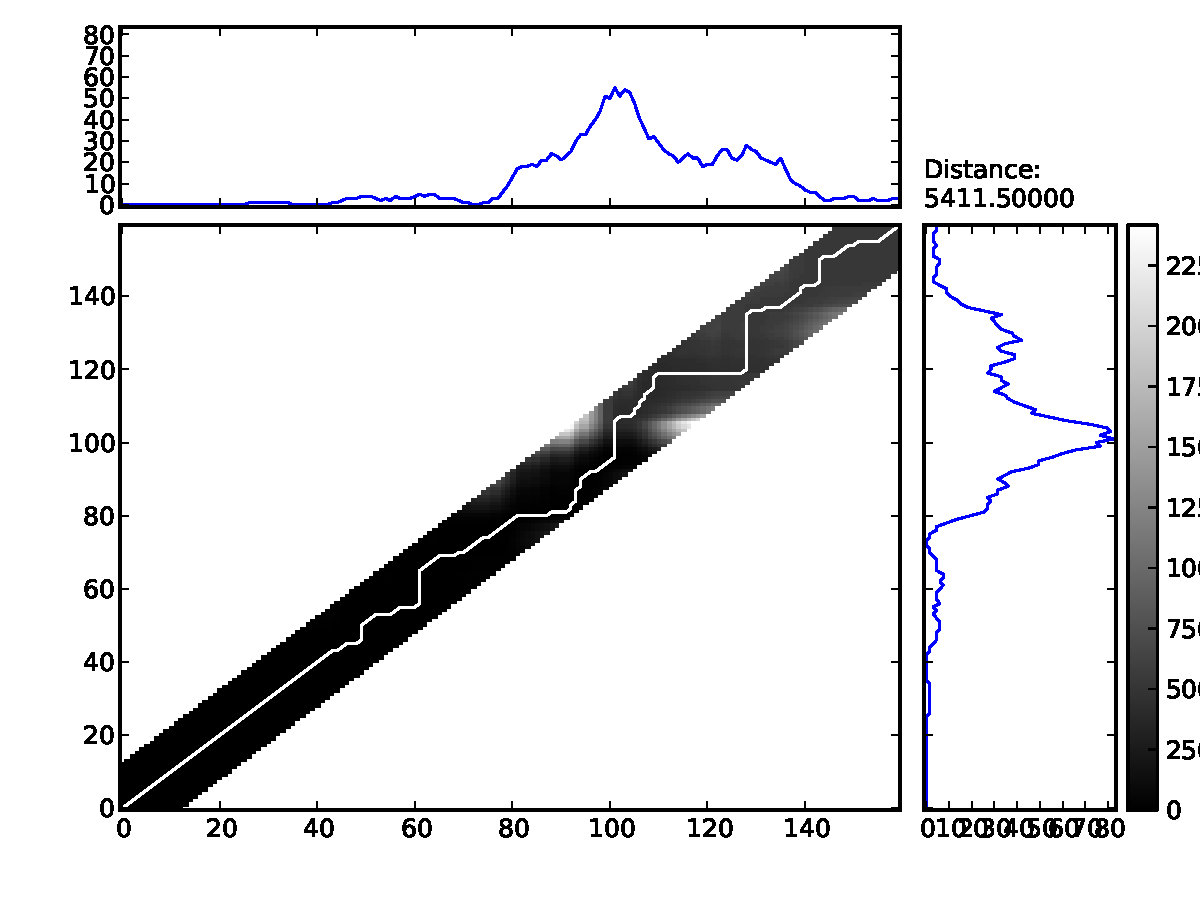
\includegraphics[width=\textwidth]{figures/methods/pileup_normalisation/cost_x_1_5_x.pdf}
       \caption{}
       \label{fig:pileup_normalisation:cost_unnormalised}
   \end{subfigure}
   ~
   \begin{subfigure}[b]{0.3\textwidth}
       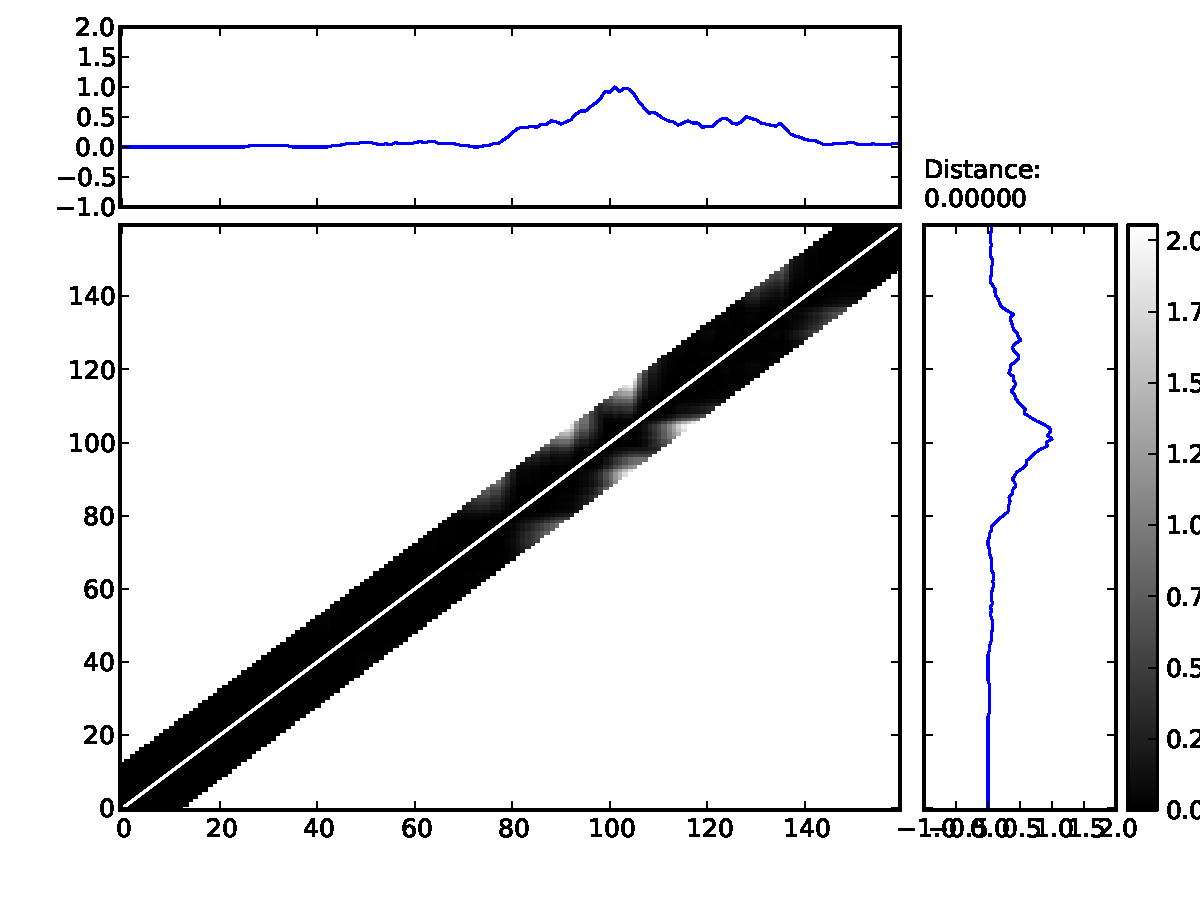
\includegraphics[width=\textwidth]{figures/methods/pileup_normalisation/cost_x_1_5_x_normalised.pdf}
       \caption{}
       \label{fig:pileup_normalisation:cost_normalised}
   \end{subfigure}
   \caption{DTW sensitivity to changes of scale. The number of reads falling to the region around transcription start site for \gene{uc003okl.3} was increased $1.5$ times. Even though this increase does not change the shape of the region (a), just the scale, the DTW distance between the original and modified regions has grown to $5411.5$ (b) which is about half of the distance between two distinct marks seen in \autoref{fig:DTW:sakoe_chiba}. A non-diagonal warping path between the regions can also be seen. After the pileup height normalisation, the distance is zero again and the path is diagonal (c).}
   \label{fig:pileup_normalisation}
\end{figure}

DTW is sensitive to changes in scale, if the local distance measure is sensitive to changes of scale.
In case of squared euclidean distance, it is very easy to artificially inflate the DTW warped distance between the two regions. For instance, consider the same region used in \autoref{fig:DTW:sakoe_chiba}. If one was to multiply all the bin counts by $1.5$, the underlying shape of the region will not change, however, as pictured in figures \ref{fig:pileup_normalisation:mappings_unnormalised} and \ref{fig:pileup_normalisation:cost_unnormalised}, the DTW distance will increase dramatically.

In some settings, e.g. differential expression studies, this might be a perfectly valid behaviour, as we might indeed want to treat these two regions as different.
In other settings, e.g. when we are trying to compare the marks at the $5'$ splicing sites, it might make more sense to compare only the shape of the mark, and not the shape and expression value. This comparison of shape can be achieved by normalising the values of the bins with the most reads falling into it to be equal to one for all regions of interest.

That is, if we thought the mark as of a vector $\mathbf{x}$, then the normalisation equation could be written as:
\begin{equation}
   \mathbf{x}_{norm} = \frac{\mathbf{x}}{max (\mathbf{x})}
\end{equation}

After the normalisation the bin with the highest number of reads in it, will always have a value equal to $1$, so the bins will be compared at the same scale. One can see the normalisation turning the distance between the original and modified regions to zero again in \autoref{fig:pileup_normalisation:cost_normalised}.

\chapter{Implementation Details}
The methods described in the previous chapter were compiled together into a software package, named Dynamic Genome Warping, or DGW for short. 

This chapter describes the implementation of this software, including its structure, interface and solutions to key computational challenges faced.

\section{Dependancies}
The core of DGW package was written in Python 2.7\footnote{See Python's homepage for more information \url{http://www.python.org/}}. The software exploits the maturing scientific community around Python and builds upon a large variety of packages produced by it.

One of the core dependancies of DGW is the \verb"pandas" package, available from \url{http://pandas.pydata.org/}. This package provides efficient, R-like data structures that are extremely easy to use. DGW uses these data structures throughout the code as to be able to both store and manipulate the histone marks efficiently. 

Packages in PyLab, namely \pythonpackage{numpy}, \pythonpackage{scipy} and \pythonpackage{matplotlib} also play a crucial part in this software. Together they bring functionality of MATLAB\footnote{See \url{http://www.mathworks.co.uk/products/matlab/} for more information about MATLAB} to Python. The first package, \pythonpackage{numpy} provides efficient computational routines on arrays and matrices; the second package, \pythonpackage{scipy} has a majority of scientific procedures available in MATLAB implemented, including the ones required for drawing and analysing hierarchical clustering dendrograms; whereas the third one, \pythonpackage{matplotlib} \cite{Hunter:2007ux}, handles all of the visualisation and plotting. 

Furthermore, Daniel M\"ullner's \pythonpackage{fastcluster} package \cite{Mullner:2011wb}, is used for efficient computations
of hierarchical clustering linkage matrices. Whereas \pythonpackage{pysam} (\url{https://code.google.com/p/pysam/}) package is used for it's Python interface to the \emph{SAMtools} (\cite{Li:2009ka}) toolkit.

Finally, implementation of the DTW algorithm is based on \pythonpackage{mlpy} package \cite{Albanese:2012vf}. The author of this project has extended this package, however, by adding support for variations of DTW algorithm described in \autoref{sec:DTW}. The author of this project has also refactored the implementation of the canonical DTW algorithm in the package as to support alignment between sequences of vectors, rather than sequences of scalars.

\section{File formats}
Since the ENCODE project, \cite{Rosenbloom:2011gw} is probably the largest repository of genomic data to date, the data formats used in this repository can be considered to be the industry standard. An exhaustive list of the data formats used in this project is provided at the FAQ section on their website, \url{https://genome.ucsc.edu/FAQ/FAQformat.html}. This section describes the two most important ones from this list, BAM and BED.

BAM file format is a successor to the SAM file format the \emph{SAMtools} toolkit is named after. The package stores the sequence alignments from a NGS experiment in a compressed binary format. Due to the amount of sequencing data generated by these experiments, BAM files are often a few gigabytes in size. 
To keep data access efficient, BAM files are often distributed along with an index file, that provides pointers to specific genetic locations in the compiled BAM file.

This format is not designed to be processed by hand, and the use \emph{SAMtools} package is suggested instead. As already described earlier, DGW uses a python wrapper around this library, \pythonpackage{pysam} to be able to extract the reads from these files.

Another file format, BED, is perfect for describing a set of genomic regions of interest, and is the default output format of the MACS peak caller due to this reason. It's structure is extremely simple: a set of tab separated fields for chromosome, start of the region, end of the region, name of the region and a few other optional fields. Due to this it is easy to parse by hand and a majority of methods that are designed to process CSV can be used to do this. 
DGW uses one of such CSV processing methods, that is implemented in \pythonpackage{pandas} to quickly load the contents of this file into \pythonpackage{pandas} data structure.

These two file formats are used for input to the software -- the ChIP-Seq datasets are expected to be in BAM format, whereas the regions of interest to cluster are expected to be in BED format.

DGW module also allows tracking of interesting locations both before and after the warping, for instance, tracking the locations of transcription start sites overlapping with clustered regions. In some cases there might be more than one such point to be tracked within the given region, e.g. more than a single transcription start site overlapping some peak called by MACS. Since BED format does not support describing disjoint regions by default, a simple file format for defining such regions was created for the sole purpose of using it in DGW. 

Each line in this file format starts with the name of the region of interest that was clustered (e.g. name of the MACS peak), followed by a colon, followed by a list of comma-separated locations of points of interest within that region, for instance:

\begin{verbatim}
MACS_peak_84:1655238,1655387,1655705,1655696,1656202
MACS_peak_86:1677162
MACS_peak_87:1689803
MACS_peak_89:1709727,1710184,1711343
\end{verbatim}

Regions that contain no such points of interest, can be safely ignored.

Even though the format is simple, it is still an \emph{ad-hoc} file format users will not be used to working with. Due to this an utility script to automatically generate points-of-interest file overlapping regions in two BED files was developed. With the help of this script, a majority of the users will not need to know how the points-of-interest file is structured as the script will do the work for them.

\section{Structure of the software}
Dynamic Time Warping is an expensive distance metric to use, as the runtime of the algorithm scales quadratically with the length of the sequences (compare this with e.g. Euclidean distance which is $O(n)$ instead). Combining that with tens of thousands regions of interest that need to be compared to each other in order to hierarchically cluster them, one will get an algorithm that is probably unlikely to be run on a laptop. 

CPU-demanding software like this is not uncommon in the field of life sciences, due to the amount of data modern experiments can produce, and therefore a majority of these labs have access to a supercomputer.

With this in mind, DGW is designed as a combination of two standalone modules: a computationally heavy module designed to be run on a supercomputer, and an exploratory module, that can analyse the results obtained from the worker module on a less-powerful computer.

\subsection{The Worker Module}
\begin{figure}
    \centering
    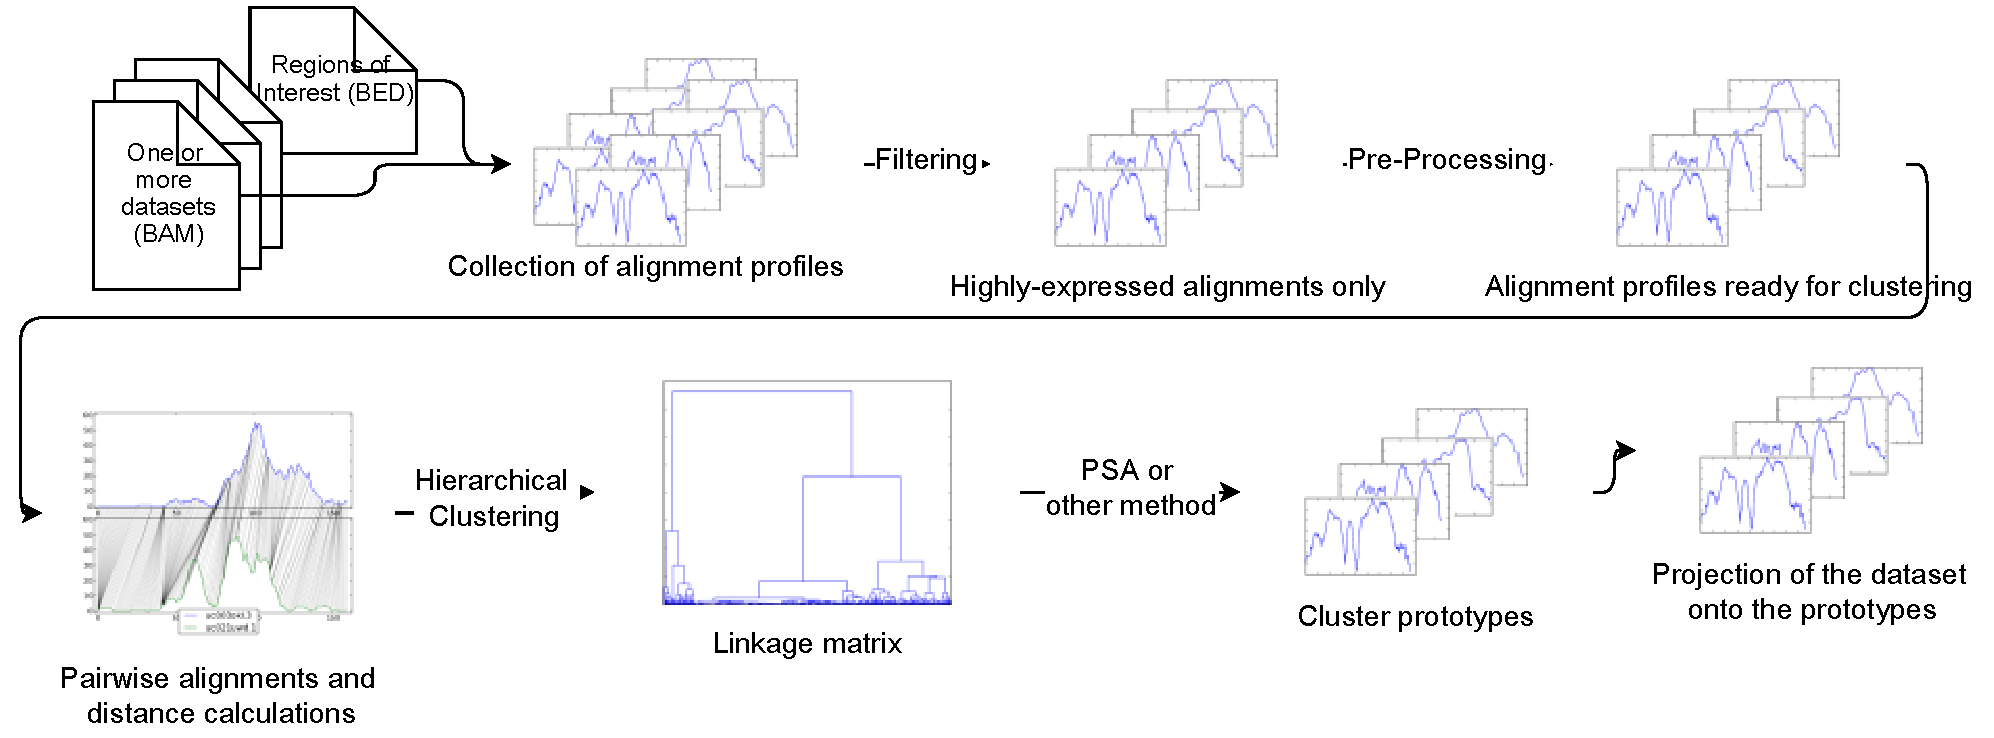
\includegraphics[width=1.1\textwidth]{figures/implementation/DGW-worker-workflow.pdf}
    \caption{Workflow of \emph{DGW-Worker} submodule. The datasets are read at the regions of interest specified by the user. Then, the resulting collection of alignment profiles is filtered leaving only highly-expressed alignments. These alignments are then pre-processed by converting them to log-scale and, optionally, normalising their values. The module then performs pairwise alignments between the items in order to calculate the pairwise distance matrix, which is then used to compute the linkage matrix for hierarchical clustering. After that, prototypes for each of the possible clusters are calculated from this linkage matrix, and the data is projected onto these prototypes.}
    \label{fig:implementation:dgw-worker-workflow}
\end{figure}

\autoref{fig:implementation:dgw-worker-workflow} outlines the workflow of the worker module.
The module first reads the regions of interest supplied by the user in a BED file. These regions are then divided into a set of bins of specified width (50 base pairs wide by default), and the histogram of number reads falling within those bins is computed, much like in \autoref{fig:background:chip-results}, to get a collection of profiles to be analysed. 

These profiles are then by keeping only the ones that have at least one bin with more than 10 reads falling into it.This filtering removes a substantial part of the dataset and thus reduces the runtime significantly. The underlying assumption of this filtering is that relatively unexpressed regions are not as interesting from the scientific point of view, and more prone to variations in patterns due to random noise. The resulting data is then converted to log scale and, optionally, normalised to be on the same scale. Please refer to \autoref{sec:reading_and_preprocessing} for an in-depth discussion of these methods.

At this point the profiles are ready to be clustered.

\subsubsection{Clustering}
During the clustering step, pairwise distances between each of the profiles are calculated.
Since this is the most time-demanding step of the algorithm, an extra effort has been put to make the clustering as efficient as it gets. 

To achieve this, the DTW clustering routines are implemented in native C. These native C modules are then called from Python code using the C-Extensions for Python suite, Cython (\url{http://www.cython.org/}). Native C code reduces the time required to compute the distance between two alignments from milliseconds to microseconds.

Microseconds might not seem much, but the number of computations that are needed to compute the pairwise distance matrix is extraordinary. If the DTW distance computation on average takes around $161$ microseconds to complete for two sequences of length 80, computing the pairwise distances for $30000$ regions would take around $20$ hours to complete as there would be ${30000 \choose 2} \approx 4.5 \times 10^8$ comparisons to make. Fortunately, computation of pairwise distances is easy to parallelise as each computation is completely independent from the others.

Parallelisation in software is usually done by splitting the execution into multiple threads.
Python supports multithreading out of the box, however, there is a catch. The Global Interpreter Lock (GIL), prohibits more than one thread interacting with the Python interpreter. Unfortunately, this means that the multithreading module is only useful for off-loading long-running non-Python procedures, such as I/O waits to a separate thread. Due to this, instead of creating new threads, parallel programs in Python create new processes each having separate Python interpreters attached to them and therefore separate GILs.

Multiprocessed architecture, however, makes sharing of information between threads challenging.
By default, Python copies the memory contents from the parent process to the child process. This behaviour is sufficient in nine cases out of ten, however, not this one. ChIP-Seq alignment profiles, once read, could take up to a few gigabytes of memory. While it is not uncommon today to see computers with 8 or more gigabytes of RAM that can easily fit datasets like this, few computers could afford copying this dataset in the memory four or more times. With this in mind, DGW implementation is careful to share critical bits of memory between the processes so the same amount of memory is used when splitting the computation between the processes.

This multiprocessing reduces the computational time by a factor equal to the number of processes used, usually upper-bounded by the number of CPUs in the computer. For instance, it would take eight times less to cluster the dataset on a machine with eight CPU cores, than it would take to cluster the same 
dataset on a computer with a single CPU only. 

The clustering step is completed by computing the hierarchical clustering linkage matrix. In order to do this, an efficient 
algorithm from the \pythonpackage{fastcluster} package is used.

\subsubsection{Prototype Generation and Data Projection}
\label{sec:prototypes}

An important property of hierarchical clustering is that there will always be $n-1$ nodes in the resulting dendrogram, where $n$ is the number of elements being clustered. This means that there are at most $n-1$ distinct clusters possible from any particular clustering of data, therefore there will at most be $n-1$ cluster prototypes possible. The worker exploits this and computes all $n-1$ prototypes using the bottom-up algorithm described in section \ref{sec:prototypes}. 

\begin{figure}[t,b]
   \centering
   \begin{subfigure}[b]{0.45\textwidth}
       \centering
       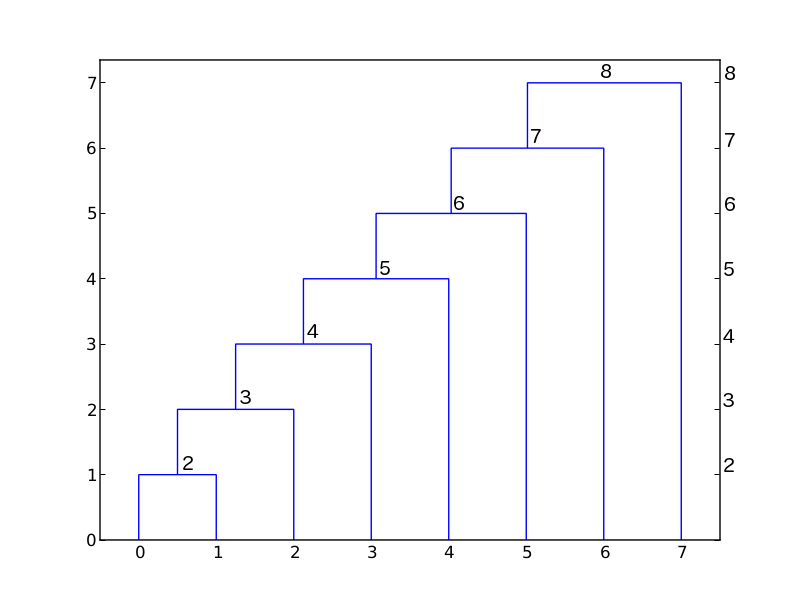
\includegraphics[width=\textwidth]{figures/implementation/worst_case_linkage.png}
       \caption{Worst case}
       \label{fig:implementation:dendrogram:worst}
   \end{subfigure}
   ~
   \begin{subfigure}[b]{0.45\textwidth}
       \centering
       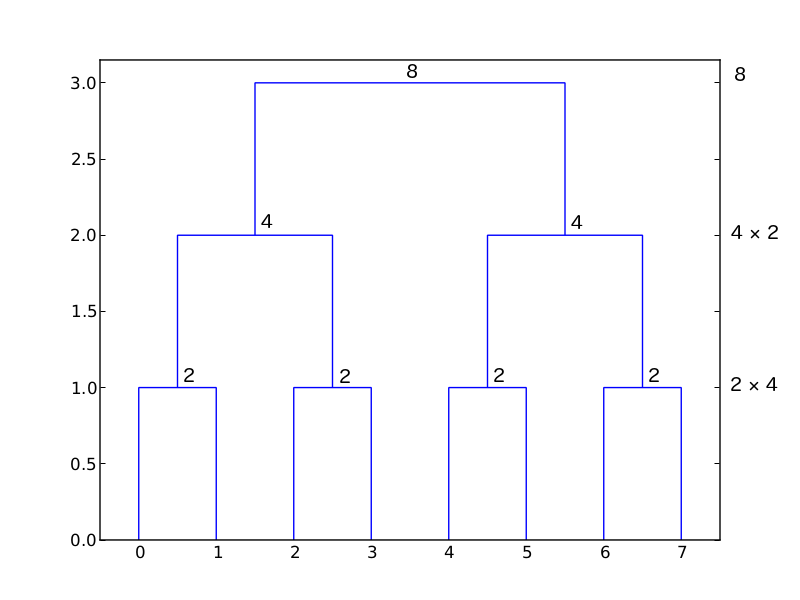
\includegraphics[width=\textwidth]{figures/implementation/perfect_linkage.png}
       \caption{Best case}
       \label{fig:implementation:dendrogram:best}
   \end{subfigure}
   \label{fig:implementation:dendrogram}
   \caption{Illustration of best-case and worst-case linkage matrices that may result from clustering of eight items. The number above the horizontal nodes corresponds to the number of items in the cluster. The number on the right side shows the number of items per level.}
\end{figure}

In order to compute the warped dataset, each element in each of the possible clusters of the dataset has to be projected onto the cluster prototype. This sounds like a tedious task, and indeed, in the worst case,  where the nodes would form a structure pictured in \autoref{fig:implementation:dendrogram:worst}, this computation would take $\frac{1}{2} n(n+1) - 1$ operations to complete, what is a bit more than ${n \choose 2}$ operations needed to compute the pairwise distance matrix. 

On the other hand, in the best case where the $n-1$ nodes would form a perfect binary tree, as pictured in \autoref{fig:implementation:dendrogram:best}, only $O(n \log n)$ DTW projection computations would be needed. Luckily, as the reader might remember from \autoref{sec:clustering}, the complete linkage criterion makes dendrograms like the one in \autoref{fig:implementation:dendrogram:worst} highly unlikely, and instead makes the dendrograms look closer to the one in \autoref{fig:implementation:dendrogram:best} on average. 

The worker module exploits this and precomputes the DTW warping paths needed to project the dataset so the worker module does not have to. Computing these paths in the worker module has another advantage of the worker being able to parallelise these tasks within the multiple CPUs of the supercomputer. Only the paths, and not the actual projections are computed, as the former takes up less memory to store. Also, having the precomputed paths allows the explorer module to be able to efficiently track locations of points-of-interest in the warped data, as described in the next section.

\subsection{The Explorer module}

\begin{figure}[p]
   \centering
       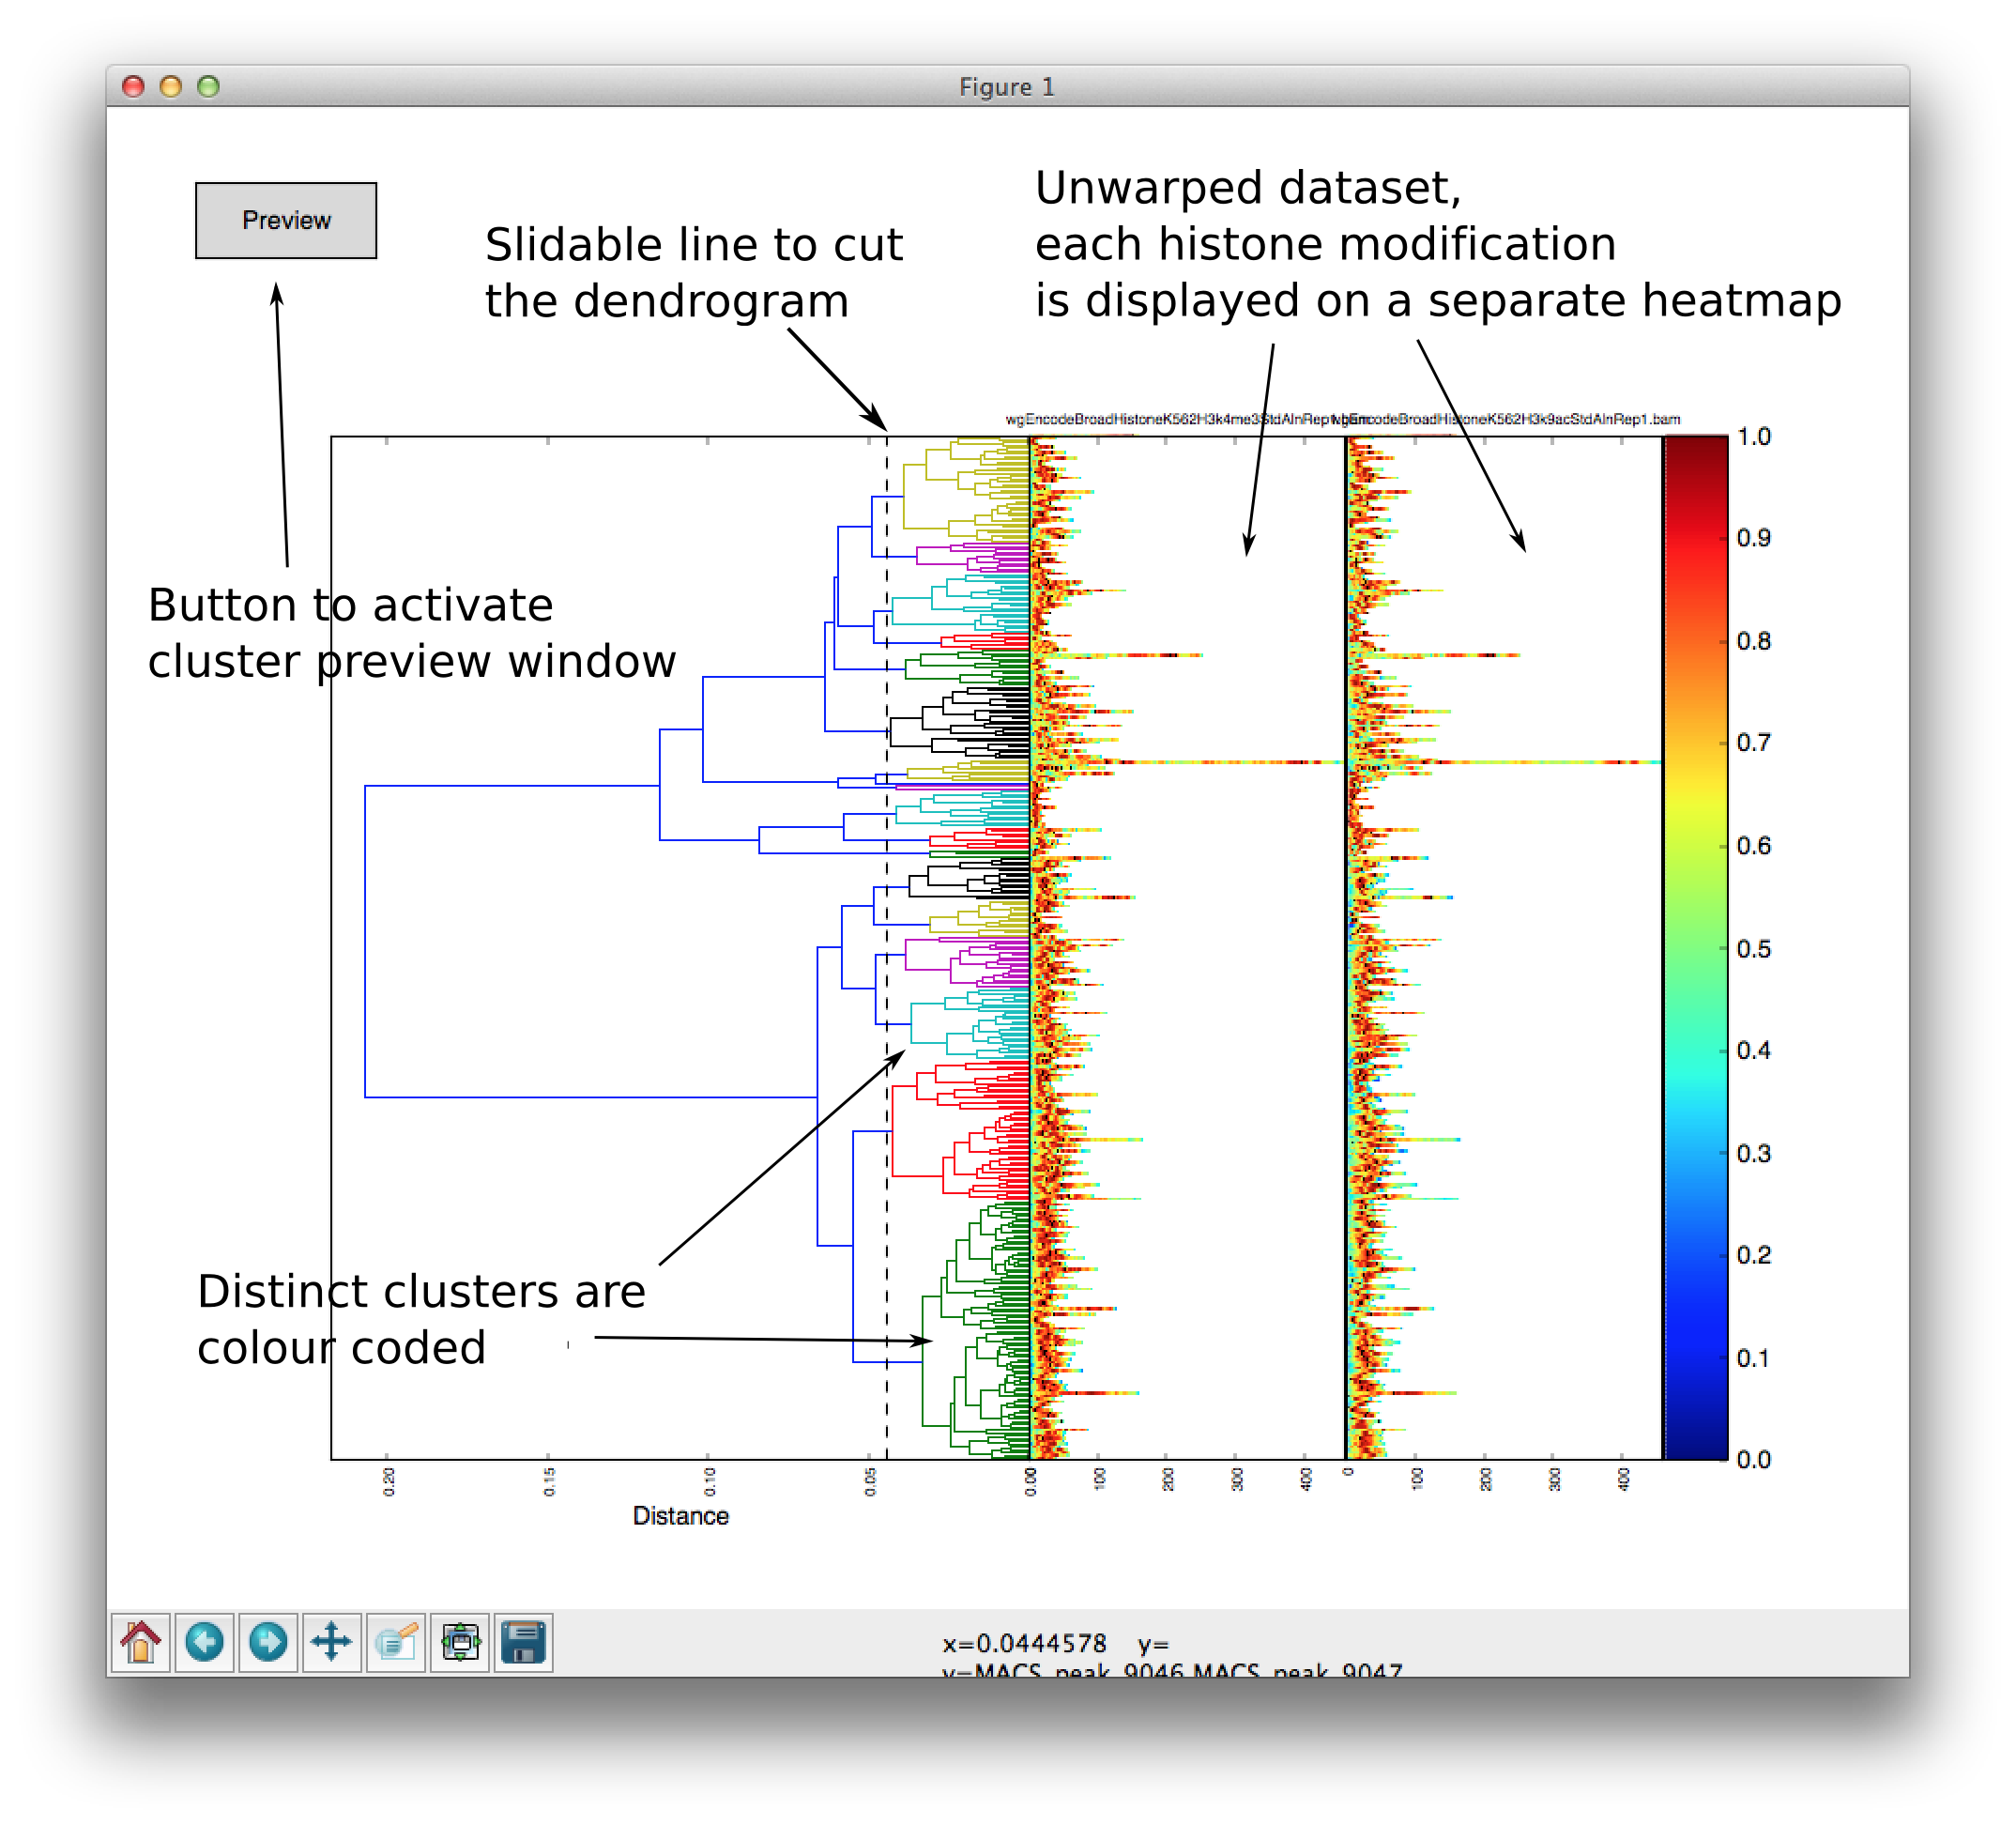
\includegraphics[height=0.45\textheight]{figures/implementation/explorer/main-window.png}
       
   \caption{Annotated screenshot of the main window of DGW-Explorer application}
   \label{fig:implementation:explorer:main}
\end{figure}

\begin{figure}[p]
    \centering
    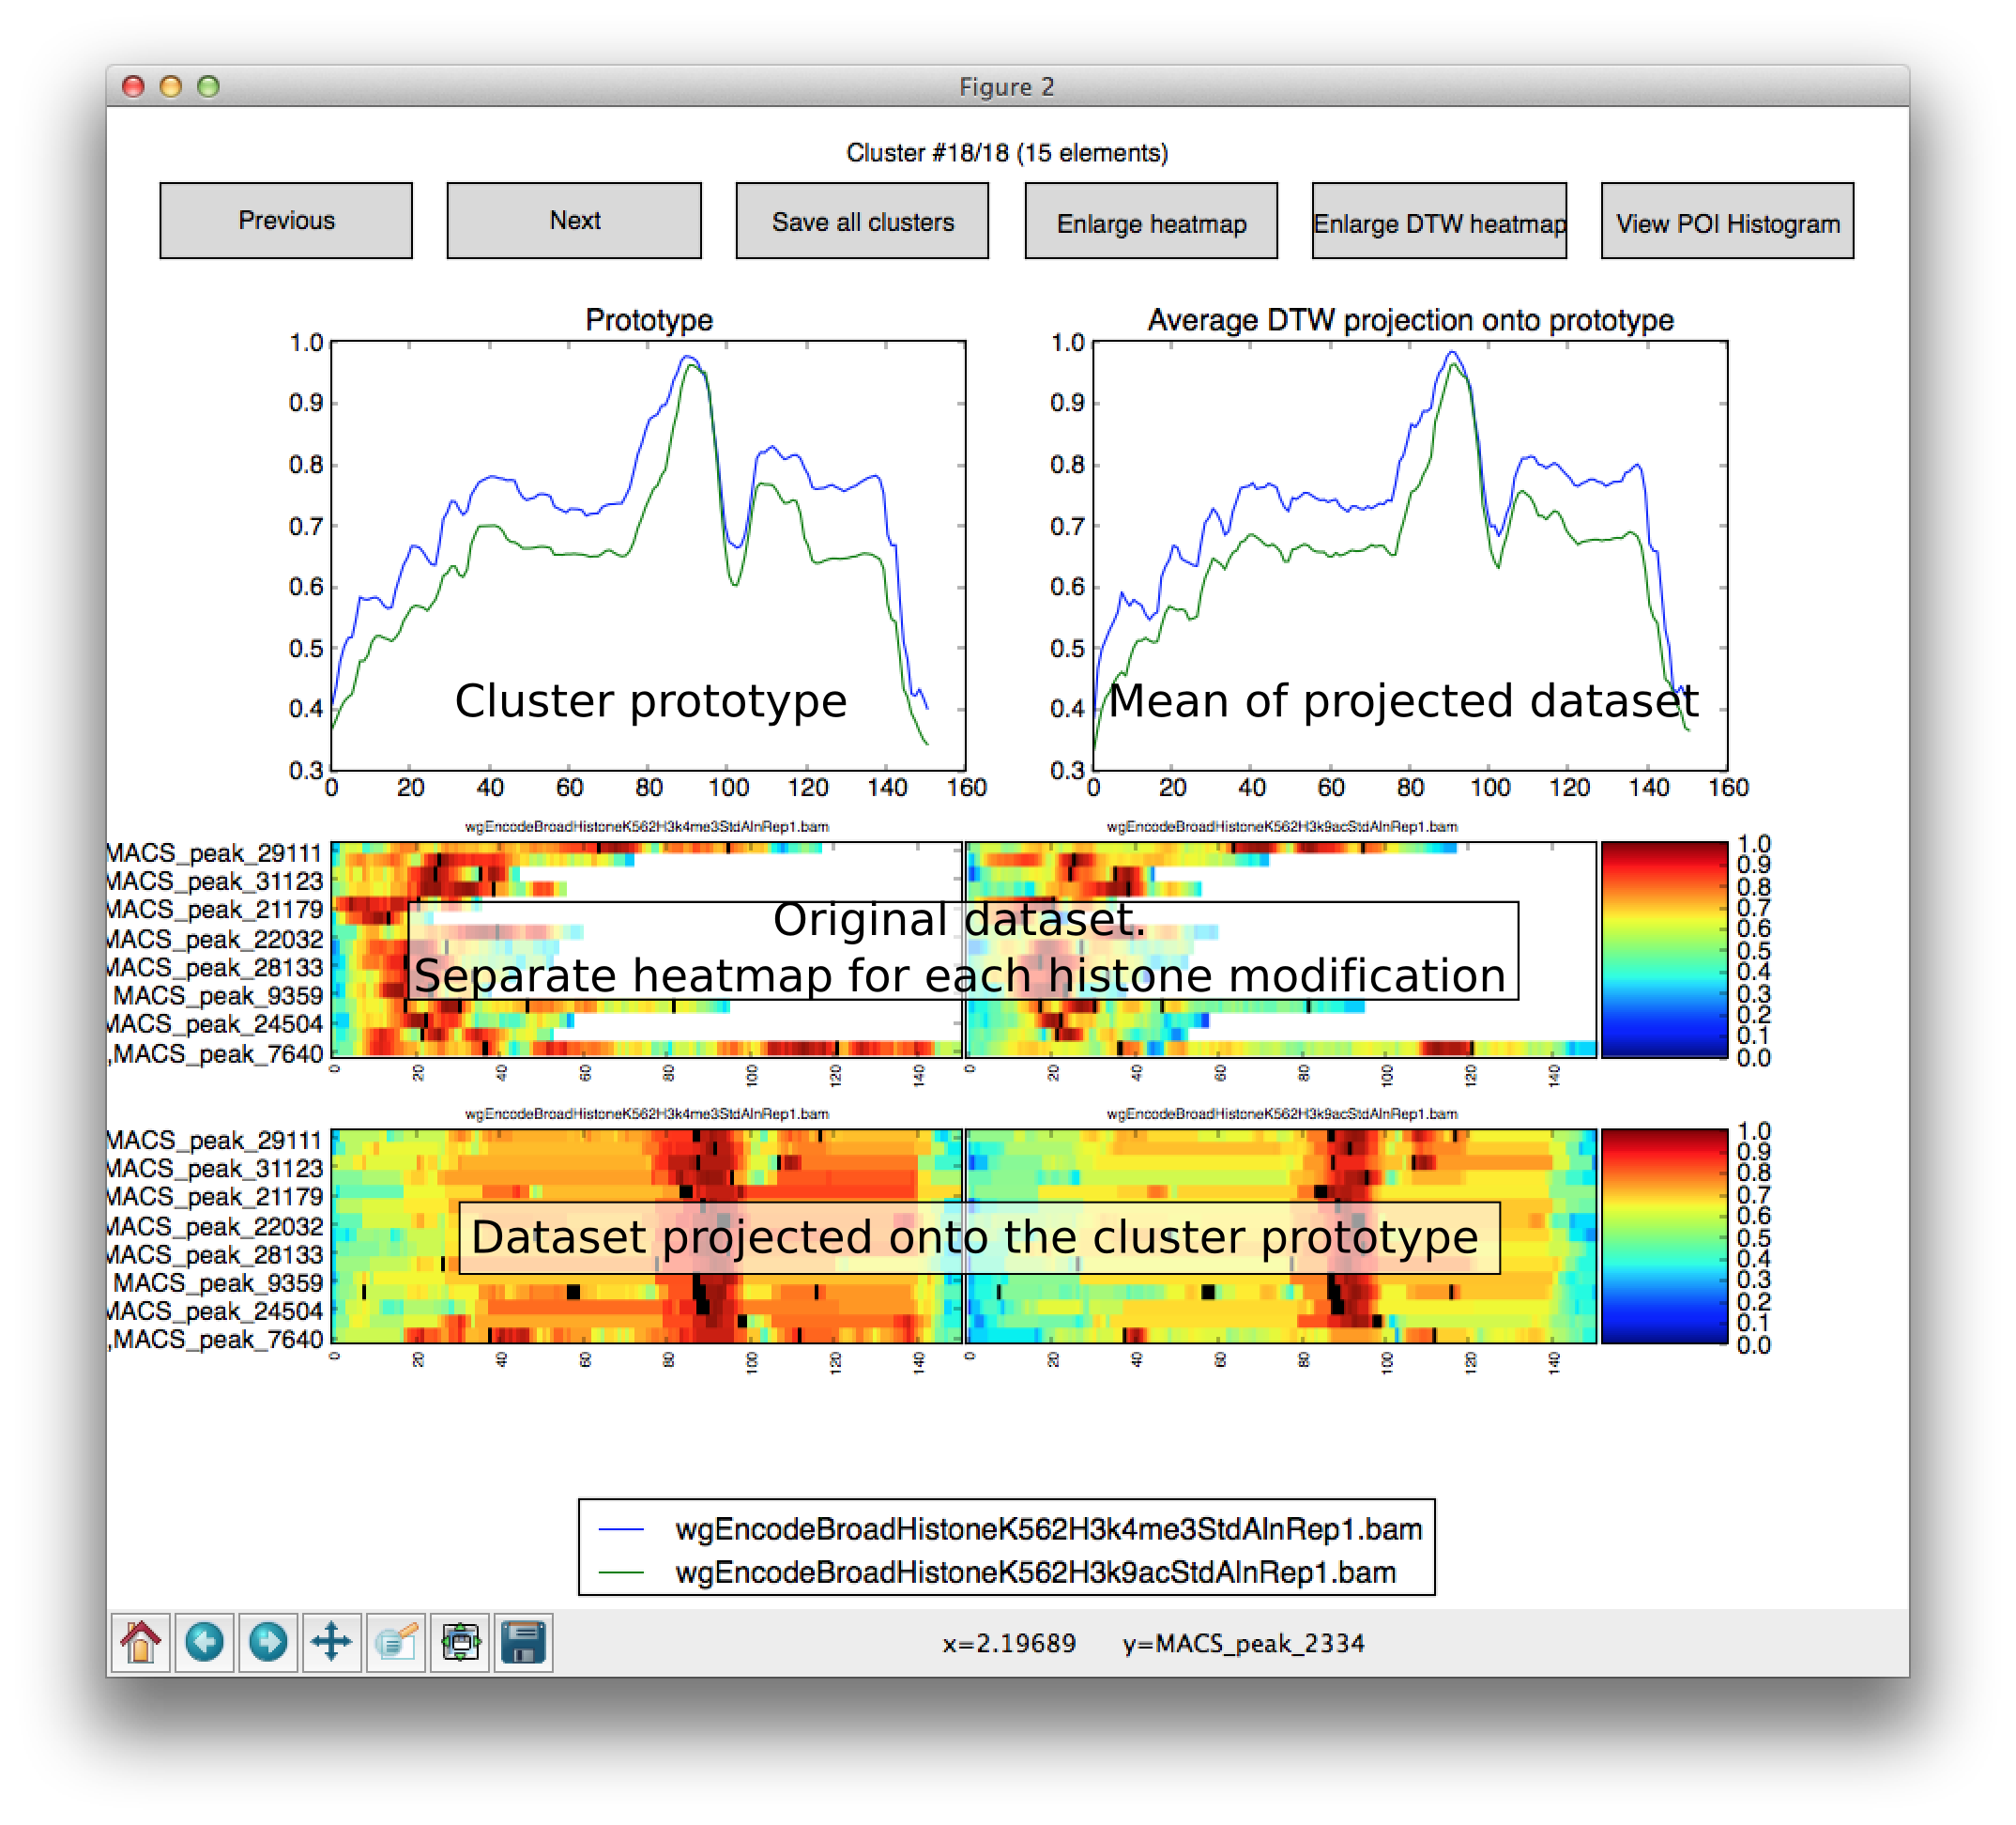
\includegraphics[height=0.45\textheight]{figures/implementation/explorer/previewer-window.png}
    \caption{Annotated screenshot of the Cluster Previewer}
    \label{fig:implementation:explorer:previewer}
\end{figure}

The explorer module is a complimentary module to the DGW-worker, that is responsible for result
visualisation and data exploration.

The main window of \emph{DGW-explorer} is shown in \autoref{fig:implementation:explorer:main}.
Here the dendrogram and zoomable heatmap of the original dataset is shown. The user is able to select the dendrogram cut threshold by simply right-clicking anywhere on the dendrogram. 
The right-click was chosen instead of left-click in order to not interfere with the default zoom controls available in the bottom-left corner of \pythonpackage{matplotlib} windows. After the dendrogram is cut, a vertical line marking the threshold is drawn and the resulting clusters are immediately colour-coded, as seen in the figure. At this stage, pressing the \emph{Preview} button, brings the Cluster Previewer window up.
 
Cluster Previewer window is pictured in \autoref{fig:implementation:explorer:previewer}.
This window summarises the clustering on a cluster-by-cluster basis. The resulting cluster prototype is shown in the top-left panel. The original data is shown below it. This dataset is then projected onto the prototype using the DTW projection technique, described in section \ref{sec:dtw-projection} and displayed in the bottom-most panel.

 The user can navigate between the clusters by the help of \emph{Previous} and \emph{Next} buttons in the top-left corner of the window, or can choose to save the clusters to a set of BED files that can then be processed by other means, e.g. viewed in the Genome Browser (\cite{Kent:2002wd}).

\subsubsection{Point-of-interest tracking}
\label{sec:poi-tracking}

The heatmap of the data projected onto the prototype is the single most useful piece of information in the cluster explorer window as it allows visual comparison of cluster items on a common ground.
In order to make these comparisons even more effective, \emph{DGW-explorer} allows the user to specify interesting genomic locations, so called points-of-interest (POI), \emph{a priori}. These locations are then marked both in the original (unwarped) and warped data heatmaps.

\begin{figure}[t,b]
   \centering
   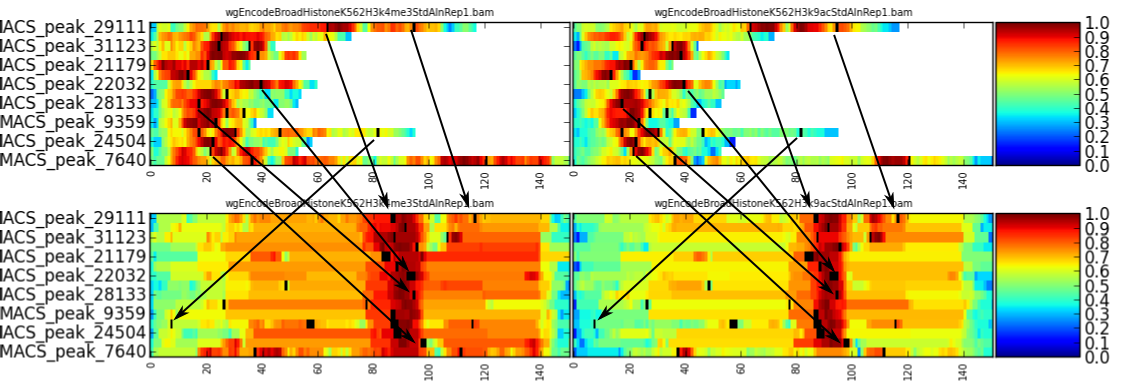
\includegraphics[width=\textwidth]{figures/implementation/explorer/poi_tracking.png}
   \caption{The heatmap part of explorer window in a close-up view. In this experiment, annotated first splicing site locations were tracked and highlighted on the heatmap as black dots. The bins containing these first splicing sites after warping are also highlighted, as seen in the figure. Black arrows were added artificially to visualise the connection between original and warped heatmaps. Note that one of the arrows is facing an opposite direction from the others, because the region was flipped during the warping.}  
   \label{fig:implementation:explorer:poi-tracking}
\end{figure}

Note that the POI locations are not used during the clustering or prototype generation and are here to merely test the hypotheses of what each of the warped patterns could mean. Since the DTW warping paths were already computed by the worker module, the POI points can be changed without rerunning the experiment, easing the testing of multiple hypotheses for the histone mark origin quickly.

The results chapter gives an example on what insights can be generated by this method.

\chapter{Results}
Evaluation of results of clustering methods has always been a challenging problem. Since clustering is unsupervised by definition, there hardly is any ground truth on what the correct way of assigning data into clusters is. One clustering might be perfectly sensible in one application, but completely useless in another. Hierarchical clustering has no clear way of deciding where dendrogram should be cut at, as already discussed earlier, making it even harder to evaluate clusterings like this. Finally, the highly exploratory goal of this project makes it even harder to sensibly evaluate the cluster assignments without doing a downstream biological analysis on them.

As previously described, Bieberstein and colleagues have shown that \histonemodification{H3K4Me3} signal peaks at the location of $5'$ splicing site \cite{Bieberstein:2012tf}. The experiments described in this chapter all inspired by these results.

\section{Clustering an Artificial Dataset}

In order to demonstrate what DGW clustering can achieve, the algorithm was tested on an artificially created dataset. In the spirit of the paper that has been mentioned previously, this artificial dataset was generated by  stretching the exon regions of a few randomly-selected genes from the UCSC known gene dataset.

More precisely, 5 genes were chosen at random. A particular care has been taken to choose among only those genes, that have their fist splicing site no further than 2000 base pairs away from the transcription start site. Alignments that fall within 2000 base pairs window around transcription start sites of these genes were read at 25 bp resolution.

The exons falling within this window were then extended randomly to be up to 60 bins, or in other words, $60 \times 25=1500$ base pairs longer. The exons were uniformly extended, keeping the shape of the underlying pattern the same, just stretched. Using this technique, dataset of size 500 was generated from the 5 seed genes depicted earlier.

These newly-generated regions were then randomly mutated, with probability of $0.33$, by changing a value of a data point, to some random value picked from the uniform distribution $U(0.5x, 1.5x)$ where $x$ is the previous value of the point. Half of these regions were then randomly reversed to generate simulate antisense patterns.

\begin{figure}[t,b]
    \centering
    \begin{subfigure}[b]{0.3\textwidth}
        \centering
        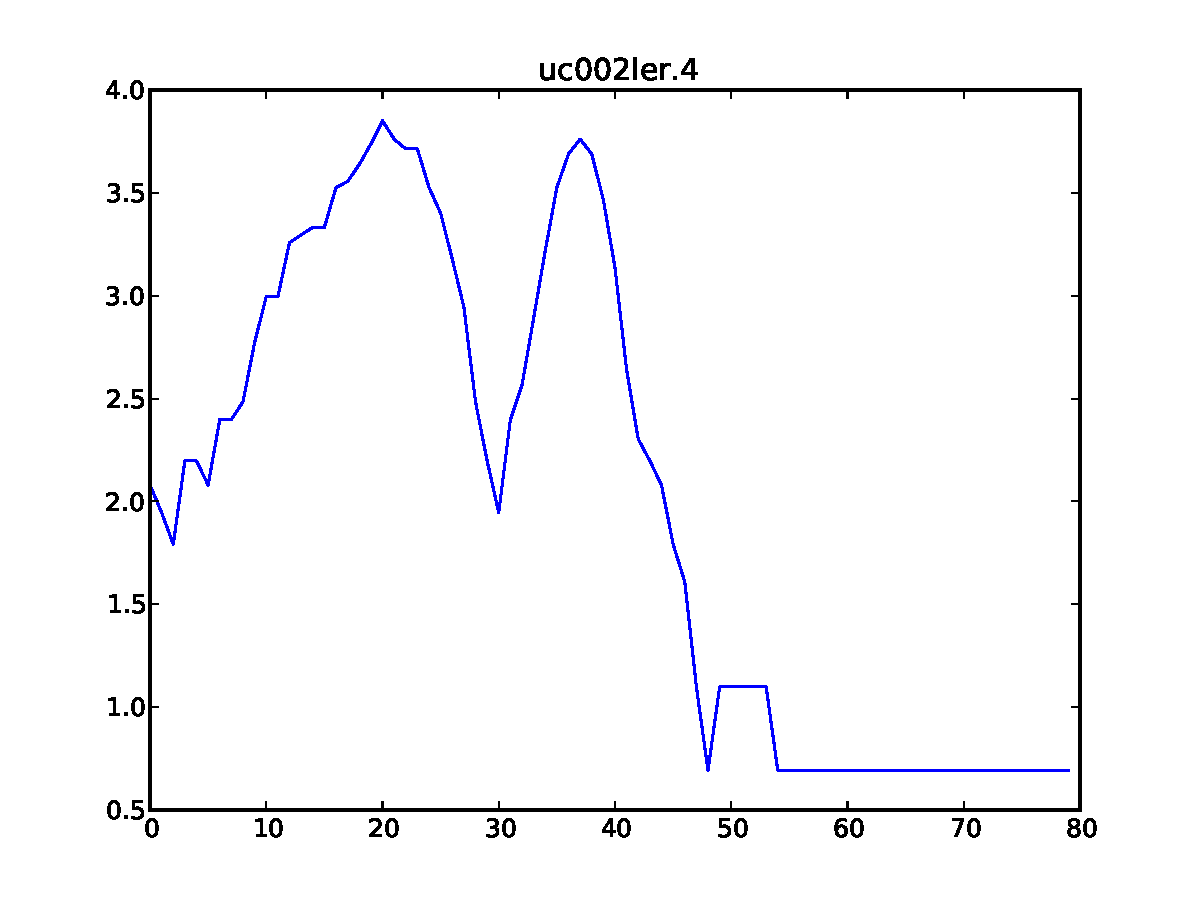
\includegraphics[width=\textwidth]{figures/evaluation/exon_stretching/uc002ler_4.pdf}
        \caption{\gene{uc001ler.4}}
        \label{fig:evaluation:exon_stretching:seeds:a}
    \end{subfigure}
    ~
    \begin{subfigure}[b]{0.3\textwidth}
        \centering
        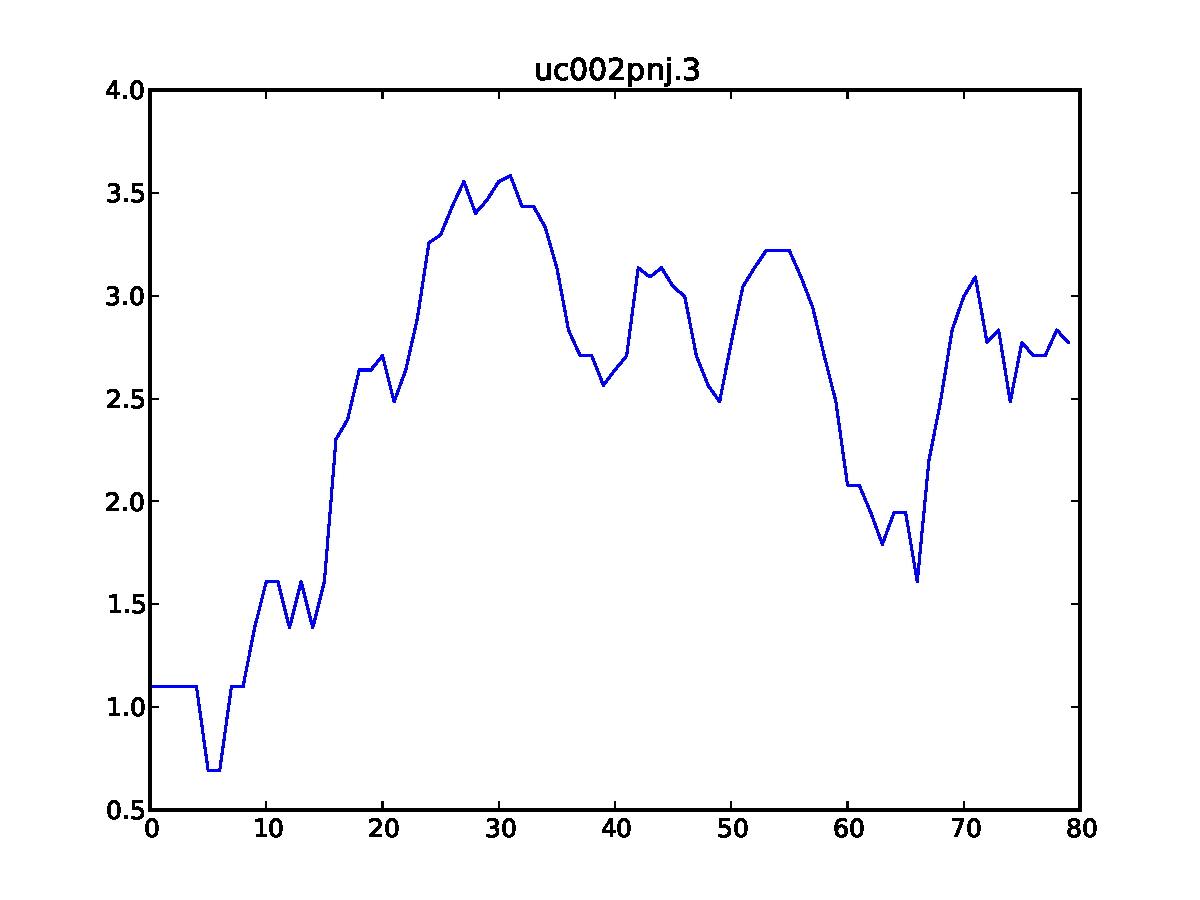
\includegraphics[width=\textwidth]{figures/evaluation/exon_stretching/uc002pnj_3.pdf}
        \caption{\gene{uc001pnj.3}}
        \label{fig:evaluation:exon_stretching:seeds:b}
    \end{subfigure}
    ~
    \begin{subfigure}[b]{0.3\textwidth}
        \centering
        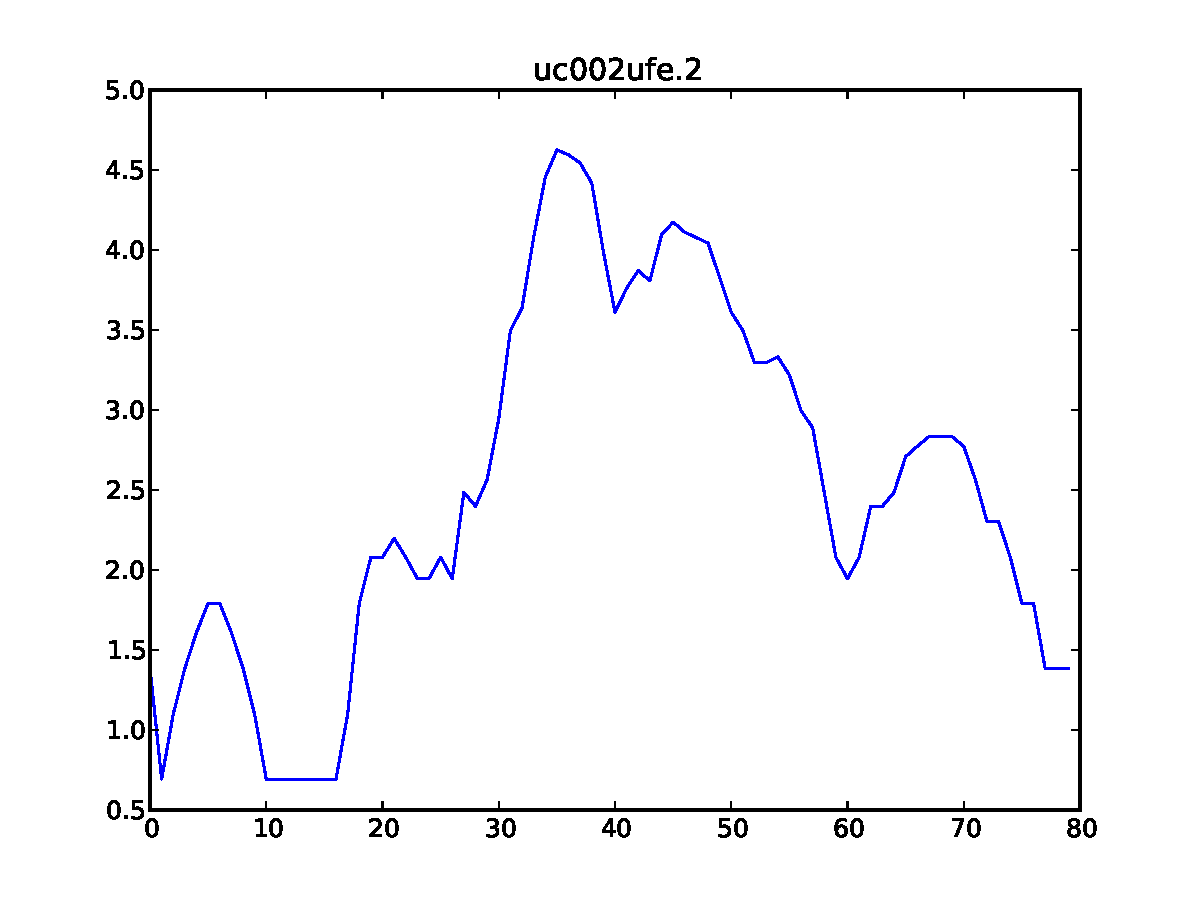
\includegraphics[width=\textwidth]{figures/evaluation/exon_stretching/uc002ufe_2.pdf}
        \caption{\gene{uc001ufe.2}}
        \label{fig:evaluation:exon_stretching:seeds:c}
    \end{subfigure}
    ~
    \begin{subfigure}[b]{0.3\textwidth}
        \centering
        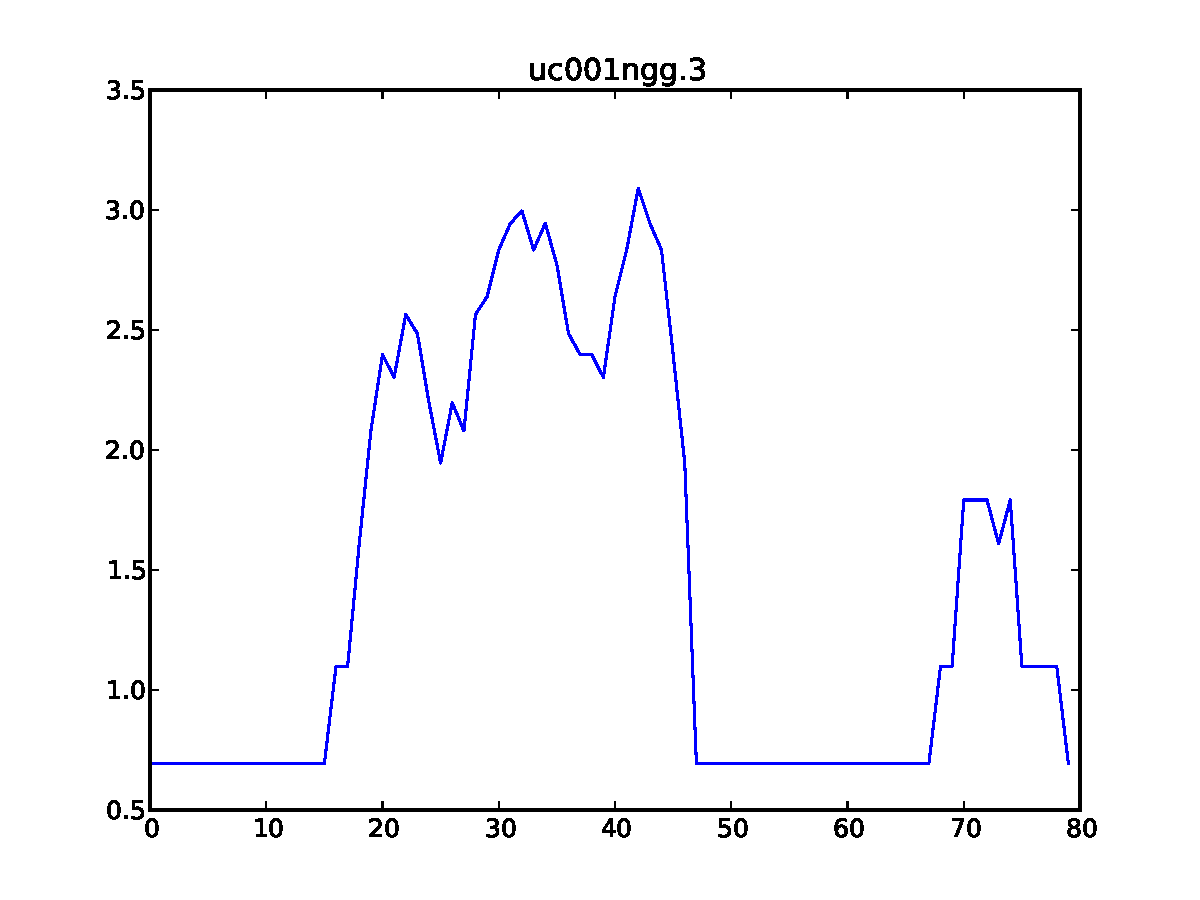
\includegraphics[width=\textwidth]{figures/evaluation/exon_stretching/uc001ngg_3.pdf}
        \caption{\gene{uc001ngg.3}}
        \label{fig:evaluation:exon_stretching:seeds:d}
    \end{subfigure}
    ~
    \begin{subfigure}[b]{0.3\textwidth}
        \centering
        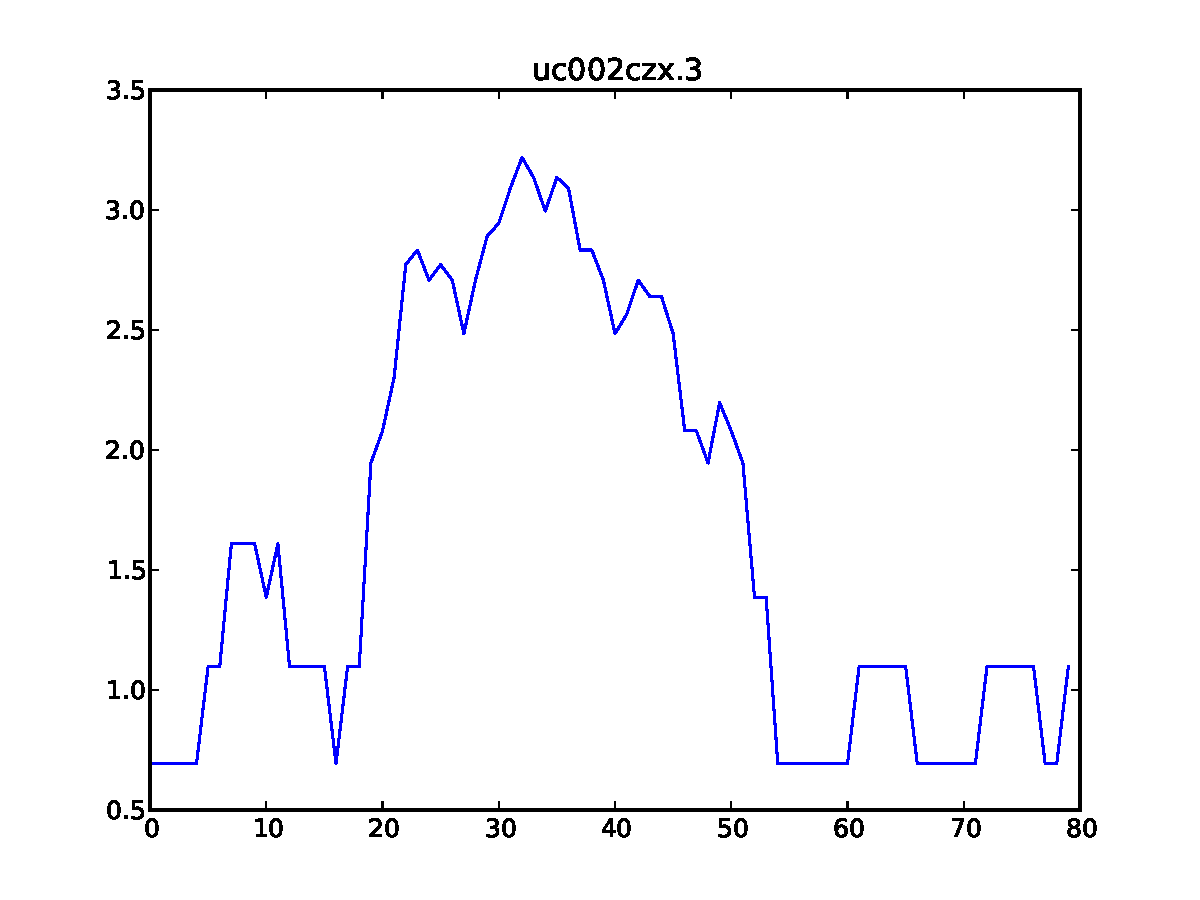
\includegraphics[width=\textwidth]{figures/evaluation/exon_stretching/uc002czx_3.pdf}
        \caption{\gene{uc001czx.3}}
        \label{fig:evaluation:exon_stretching:seeds:e}
    \end{subfigure}
    \caption{The five seed regions that were used to generate the artificial dataset. Note the similarity between the patterns in \ref{fig:evaluation:exon_stretching:seeds:d} and \ref{fig:evaluation:exon_stretching:seeds:e}, i.e. if one of the patterns was reversed}
    \label{fig:evaluation:exon_stretching:seeds}
\end{figure}

\autoref{fig:evaluation:exon_stretching:seeds} shows the five seed patterns that were selected. 
Notice that two of them, namely \gene{uc001ngg.3} (\autoref{fig:evaluation:exon_stretching:seeds:d}) and \gene{uc001czx.3} (\autoref{fig:evaluation:exon_stretching:seeds:e}) seem to have a relatively similar mark: the former having a large peak followed by a smaller one, whereas the latter having a smaller peak followed by a larger one. Intuitively, we would expect the algorithm to be able to join the items generated from these two samples relatively early.

\begin{figure}[t,b]
   \centering
   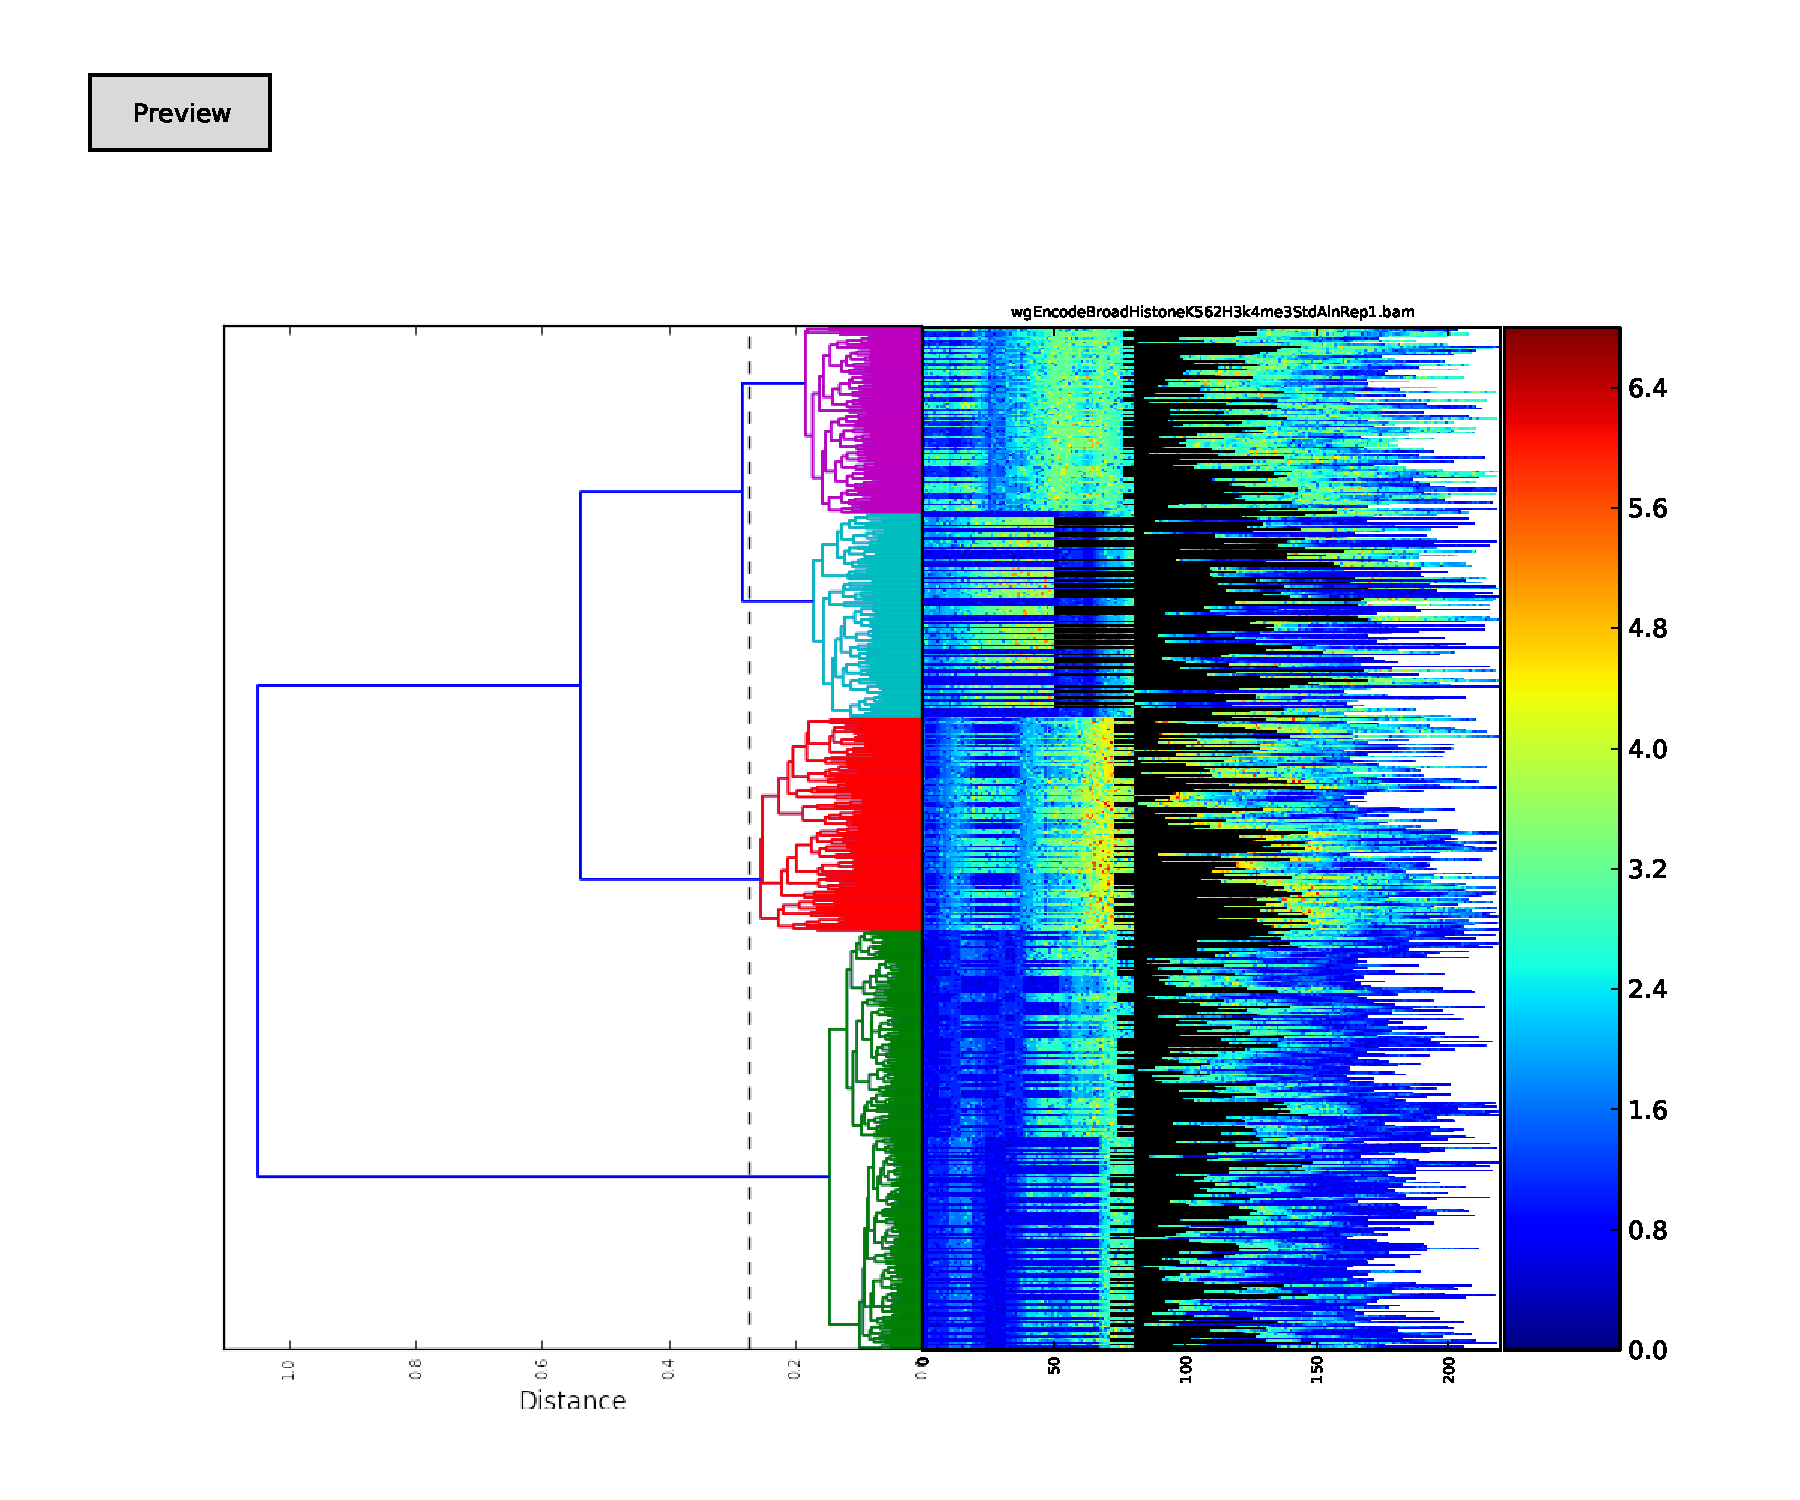
\includegraphics[width=\textwidth]{figures/evaluation/exon_stretching/dgw_cut.pdf}
   \caption{Result of clustering the dataset that was generated by stretching exon regions from the five seed samples in \autoref{fig:evaluation:exon_stretching:seeds}. The extended exons are marked as black points in the heatmap.}
   \label{fig:evaluation:exon_stretching:cut}
\end{figure}

\begin{figure}[t,b]
    \centering
    \begin{subfigure}[b]{0.22\textwidth}
        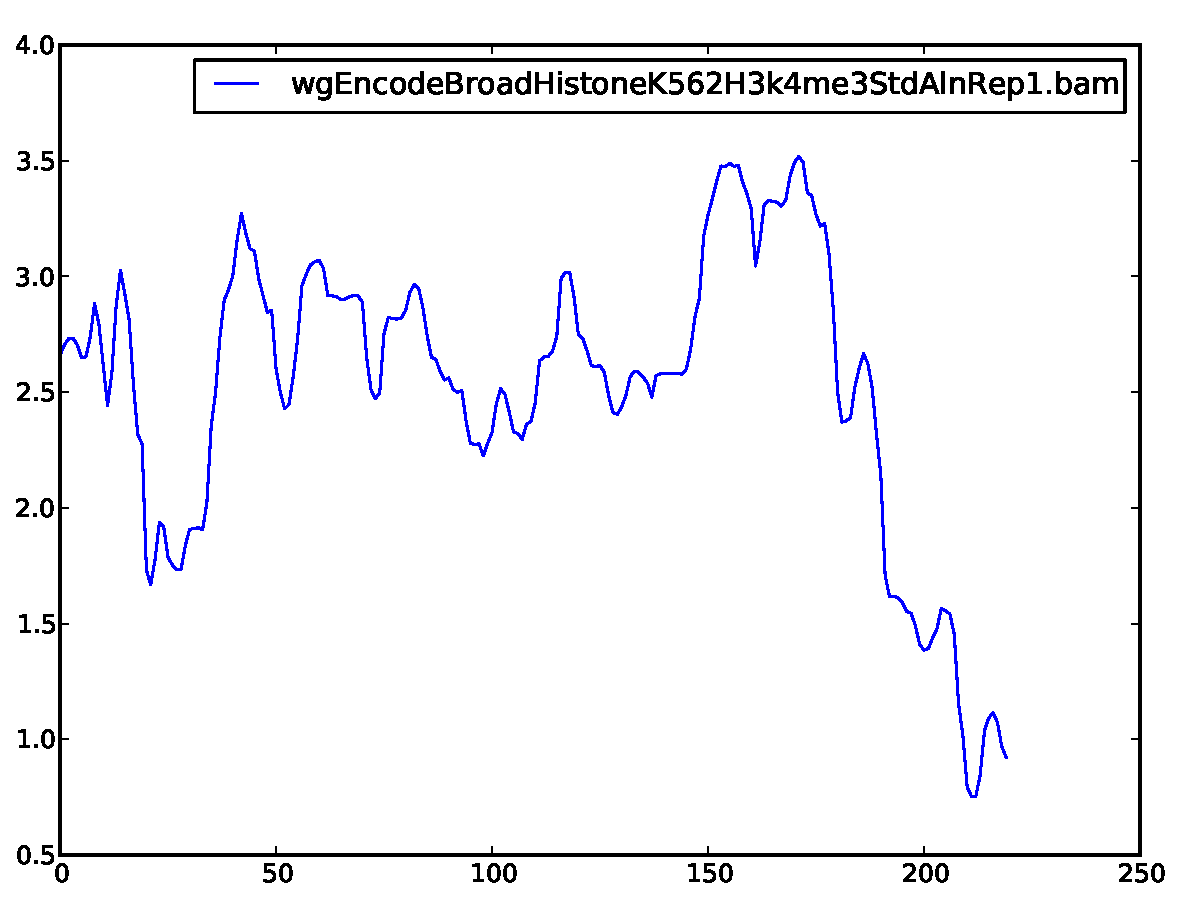
\includegraphics[width=\textwidth]{figures/evaluation/exon_stretching/cluster-2.pdf}
        \caption{Purple cluster prototype}
        \label{fig:evaluation:exon_stretching:clusters:1:prototype}
    \end{subfigure}
    ~
    \begin{subfigure}[b]{0.22\textwidth}
        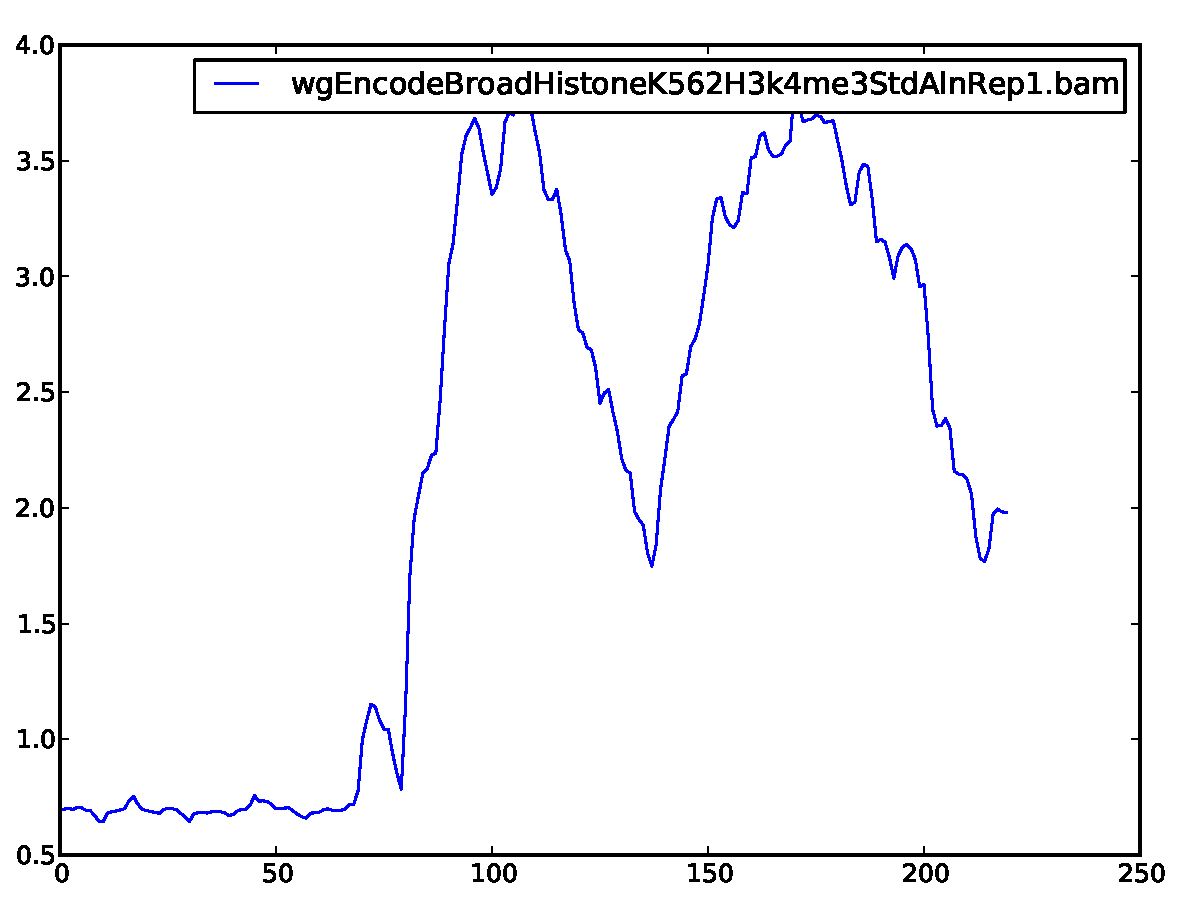
\includegraphics[width=\textwidth]{figures/evaluation/exon_stretching/cluster-1.pdf}
        \caption{Cyan cluster prototype}
        \label{fig:evaluation:exon_stretching:clusters:2:prototype}
    \end{subfigure}
    ~
    \begin{subfigure}[b]{0.22\textwidth}
        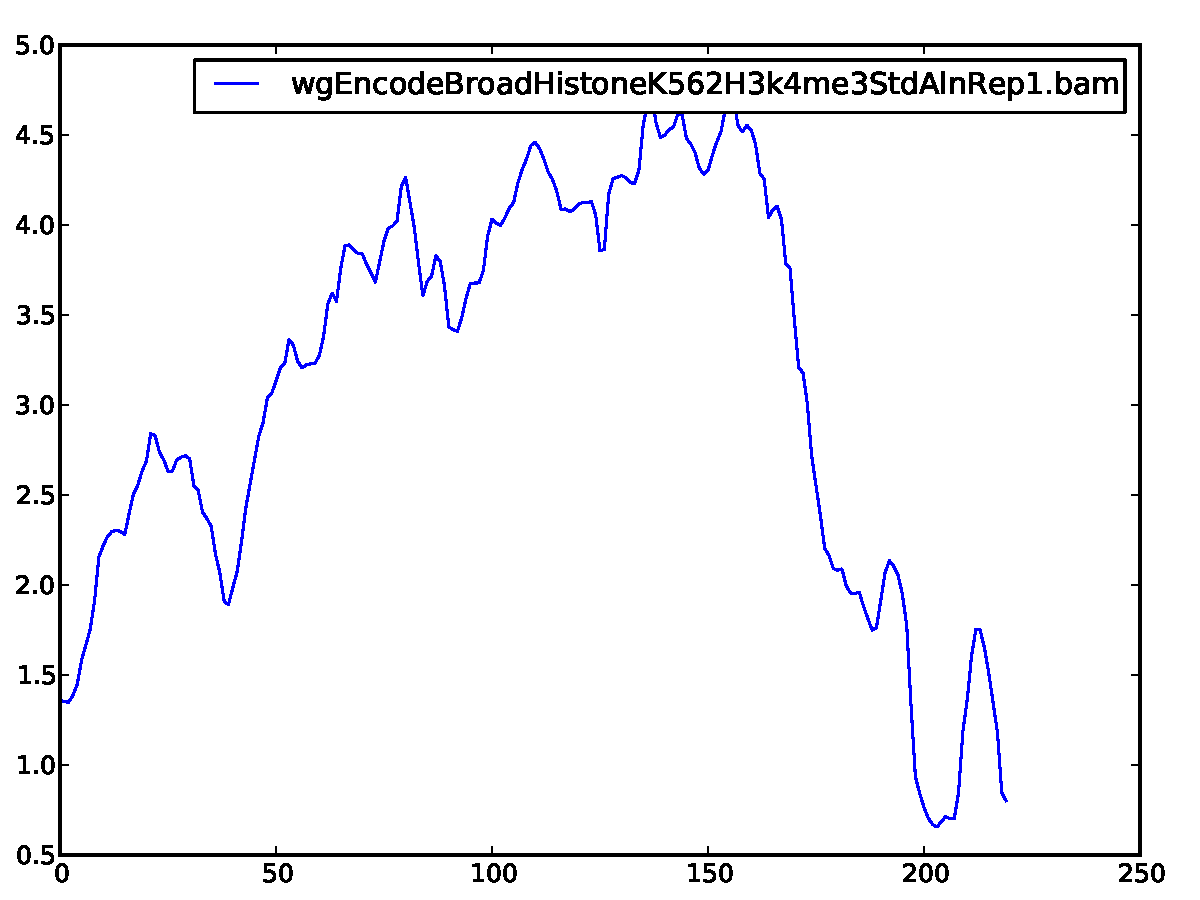
\includegraphics[width=\textwidth]{figures/evaluation/exon_stretching/cluster-4.pdf}
        \caption{Red cluster prototype}
        \label{fig:evaluation:exon_stretching:clusters:3:prototype}
    \end{subfigure}
    ~
    \begin{subfigure}[b]{0.22\textwidth}
        \includegraphics[width=\textwidth]{figures/evaluation/exon_stretching/cluster-3.pdf}
        \caption{Green cluster prototype}
        \label{fig:evaluation:exon_stretching:clusters:4:prototype}
    \end{subfigure}
    \caption{Prototypes of the four clusters resulting from the dendrogram in \autoref{fig:evaluation:exon_stretching:cut}. Note how closely they resemble the five seed motifs in \autoref{fig:evaluation:exon_stretching:seeds}.}
    \label{fig:evaluation:exon_stretching:clusters:prototypes}
\end{figure}

And indeed, the dendrogram in \autoref{fig:evaluation:exon_stretching:cut} shows the resulting hierarchical clustering of these regions. Only four distinct clusters were created at the selected cut threshold, because the items from two similar prototypes were joined into the largest green cluster earlier than other clusters were formed. 

This early merging can be explained by the nature of the mutation function that is being used in this experiment: since the level of mutation depends on the actual value of the point being mutated, seed regions that have a majority of regions expressed poorly, will undergo less mutation than highly-expressed regions, due to this the distance at which they are joined will be lower. 

Despite the early merging, the prototypes of these four clusters, pictured in  \autoref{fig:evaluation:exon_stretching:clusters:prototypes}, seem to more or less resemble the seed motifs in the figure \autoref{fig:evaluation:exon_stretching:seeds}. The prototype for the green cluster seems to join the seed motifs \gene{uc001ngg.3} and \gene{uc001czx.3} together by averaging the features that occur in both of them.

\begin{figure}[t,b]
    \centering
    \begin{subfigure}[b]{0.22\textwidth}
        \includegraphics[width=\textwidth]{figures/evaluation/exon_stretching/cluster-warped-2.pdf}
        \caption{Purple cluster}
        \label{fig:evaluation:exon_stretching:clusters:1:warped}
    \end{subfigure}
    ~
    \begin{subfigure}[b]{0.22\textwidth}
        \includegraphics[width=\textwidth]{figures/evaluation/exon_stretching/cluster-warped-1.pdf}
        \caption{Cyan cluster}
        \label{fig:evaluation:exon_stretching:clusters:2:warped}
    \end{subfigure}
    ~
    \begin{subfigure}[b]{0.22\textwidth}
        \includegraphics[width=\textwidth]{figures/evaluation/exon_stretching/cluster-warped-4.pdf}
        \caption{Red cluster}
        \label{fig:evaluation:exon_stretching:clusters:3:warped}
    \end{subfigure}
    ~
    \begin{subfigure}[b]{0.22\textwidth}
        \includegraphics[width=\textwidth]{figures/evaluation/exon_stretching/cluster-warped-3.pdf}
        \caption{Green cluster}
        \label{fig:evaluation:exon_stretching:clusters:4:warped}
    \end{subfigure}
    \caption{Data dynamically warped onto the prototypes. Exon locations are marked in black. Note the clear split between two seed motifs that are combined into the green cluster.}
    \label{fig:evaluation:exon_stretching:clusters:warped}
\end{figure}

Looking at the DTW projections of the data onto these cluster prototypes in \autoref{fig:evaluation:exon_stretching:clusters:warped}, it can be seen that the exons (marked in black) align more or less after the warping, with some slight inaccuracies due to the artificial mutations of the dataset. 

Since items in these heatmaps are in the same order as they were in the dendrogram, the separation between two subclusters forming the green cluster is very clear in the heatmap as well as seen in\autoref{fig:evaluation:exon_stretching:clusters:4:warped}. Note that is clear that items of one of the seed patterns were reversed to align better with the items from the other seed pattern. This can be seen by looking at the positions of the exons of the two subclusters.

\section{Clustering the Results of a Peak Caller}
\label{sec:macs-experiment}
Tests on the artificial benchmark have shown that the DGW algorithm is able to do what it says on the label. However, this does not give any insights on the whether the method will prove useful for actual research. In order to test this, an experiment to simulate a scenario that is likely to occur in research was created.

In this experiment, MACS peak caller with default configuration \cite{Zhang:2008wp} was run on the ChIP-Seq results for \histonemodification{H3K4Me3} marks in \celltype{K562} cell type. Data from the control ChIP-Seq experiment was used to allow MACS anticipate between significantly and insignificantly enriched regions relative to the control.

The output of this peak caller was then preprocessed by joining together resulting regions that are within 50bp of each other, using {\tt BEDTools} package \cite{Quinlan:2010ur}. 
All transcription start sites and first splicing sites that overlap these regions were identified and compiled into a list of points of interest. Regions containing no such points of interest were dropped.

Then the datasets for \histonemodification{H3K4Me3} and \histonemodification{H3K9Ac} histone modifications, the same histone modifications that were observed to peak at first splicing sites by \cite{Bieberstein:2012tf}, were read to generate multidimensional histone profiles for these regions.

Histone marks at the regions of interest were then clustered by DGW at the resolution of 50 base pairs per bin. Squared euclidean distance was selected to be the local distance measure and slanted band constraint of width 12, as described in \autoref{sec:slanted-band-constraint} was chosen. The maximum histogram heights were all normalised to be equal to one as described in \autoref{sec:pileup_height_normalisation}.

\autoref{fig:evaluation:macs-peaks:cut} shows the resulting dendrogram and the chosen cut. Explorer window for one of the clusters is pictured in \autoref{fig:evaluation:macs-peaks:explorer}. Note the highly varying lengths of the peaks in the original data. \autoref{fig:evaluation:macs-peaks:warped-heatmap} shows enlarged heatmap of the data projected onto the cluster prototype. Here, the heatmap of the left represents the projected \histonemodification{H3K4Me3} mark, whereas the heatmap on the right corresponds to \histonemodification{H3K9Ac}. 

Looking closely, it can be seen that the first splicing sites (marked in black) are aligned to the same location after warping. \autoref{fig:evaluation:macs-peaks:histogram-warped} quantifies this alignment by plotting the points-of-interest distribution for each of the warped bins. The top panel corresponds to the distribution of $5'$ splicing sites, whereas the bottom one corresponds to the transcription start site distribution. From this figure, and from the heatmap, it is clear that not only first splicing sites are aligned, but also the transcription start site locations are aligned a few bins to the right from the $5'$ splicing site.

This alignment is not visible in the original data, as pictured in \autoref{fig:evaluation:macs-peaks:histogram-original}. In order to generate this histogram, the regions were stretched to match the length of the longest region first, using a procedure similar to the one used to stretch the exons in the previous experiment. The distributions for these stretched regions were then computed in the same way as for warped data.

\begin{figure}
    \centering
    \begin{subfigure}[b]{0.45\textwidth}
         \includegraphics[width=\textwidth]{figures/evaluation/macs-peaks/cut-no-preview-button.png}
         \caption{Resulting Dendrogram}
         \label{fig:evaluation:macs-peaks:cut}
    \end{subfigure}
    ~
    \begin{subfigure}[b]{0.5\textwidth}
        \centering
        \includegraphics[width=\textwidth]{figures/evaluation/macs-peaks/dgw-explorer-cluster-35.png}
        \caption{Explorer window for cluster 35}
        \label{fig:evaluation:macs-peaks:explorer}
    \end{subfigure}
    ~
    \begin{subfigure}[b]{0.8\textwidth}
        \includegraphics[width=\textwidth]{figures/evaluation/macs-peaks/dgw-cluster-35-warped-heatmap.pdf}
        \caption{Cluster data projected onto the cluster prototype. First splicing sites are marked in black, whereas the trasncription start sites are marked in white.}
        \label{fig:evaluation:macs-peaks:warped-heatmap}
    \end{subfigure}
    ~
    \begin{subfigure}[b]{0.3\textwidth}
        \centering
        \includegraphics[width=\textwidth]{figures/evaluation/macs-peaks/cluster-35-histogram-clean.png}
        \caption{Distribution of POI before warping.}
        \label{fig:evaluation:macs-peaks:histogram-original}
    \end{subfigure}
    ~
    \begin{subfigure}[b]{0.3\textwidth}
         \centering
        \includegraphics[width=\textwidth]{figures/evaluation/macs-peaks/cluster-35-warped-histogram-clean.png}
        \caption{Distribution of POI after warping.}
        \label{fig:evaluation:macs-peaks:histogram-warped}
    \end{subfigure}
    \caption{Results of clustering the peaks found by MACS peak caller. Transcription start sites are marked in white and the first splicing sites are marked in black in the heatmaps. The two histograms in \ref{fig:evaluation:macs-peaks:histogram-original} and \ref{fig:evaluation:macs-peaks:histogram-warped} show the distribution of the number of regions containing a transcription start site or a first splicing site in each of the bins. For original data, all regions were stretched to be of the same length before calculating the distributions.}
    \label{fig:evaluation:macs-peaks}
\end{figure}

\section{Distinct Patterns Around Transcription Start Sites}
\label{sec:evaluation:tss}

The final experiment is designed to test DGW's ability to identify and visualise the distinct patterns within the regions of interest. In this experiment, well documented regions around transcription start sites were clustered.

More specifically, 2000 base pair windows around the transcription start sites of UCSC known genes dataset (see \autoref{sec:datasets}) were selected. If two regions were overlapping each other, both of them were discarded as to only leave regions that contain a single transcription start site and no other transcription start sites in the neighbourhood.

The data at these specific regions was extracted from the ENCODE \histonemodification{H3K4Me3} dataset for the K562 leukaemia cell line at the resolution of 25 base pairs per bin. Before processing, the dataset was normalised as described in \autoref{sec:pileup_height_normalisation}.
This data was then clustered using DTW constrained with slanted band of size 12.

The resulting dendrogram can be seen in \autoref{fig:evaluation:tss_regions:cut}. Looking at the cluster prototypes, pictured in \autoref{fig:evaluation:tss_regions:prototypes}, the well-known bimodal patterns around TSS can be seen in figures \ref{fig:evaluation:tss_regions:prototypes:c}, \ref{fig:evaluation:tss_regions:prototypes:d} and \ref{fig:evaluation:tss_regions:prototypes:e}.
\ref{fig:evaluation:tss_regions:prototypes:j}.

Perhaps more interestingly, a few unusual patterns can be seen from the prototypes.
For instance, the pattern in \ref{fig:evaluation:tss_regions:prototypes:b} has two distinct valleys,
rather than one.
Prototypes of clusters pictured in \ref{fig:evaluation:tss_regions:prototypes:f}, \ref{fig:evaluation:tss_regions:prototypes:g} and  \ref{fig:evaluation:tss_regions:prototypes:i} seem to be much more narrow than the remaining clusters, with only a little evidence of bimodality. 

These patterns can be studied in help with the cluster heatmaps, pictured in 
Figures \ref{fig:evaluation:tss_regions:heatmaps:unwarped} and \ref{fig:evaluation:tss_regions:heatmaps:warped}.

Note that common patterns between the regions can be spotted by inspecting the original data visually. 
This is because the experiment was designed with this in mind: regions are all of the same length, and share a common landmark -- the transcription start site in the middle. In a general case, one would not not have such luxury, as seen in the previous experiment where MACS peaks were clustered.

Now if the patterns were identifiable from the original data, they are unmistakable in the warped data. For instance, the regions in \autoref{fig:evaluation:tss_regions:heatmaps:unwarped:a} look bimodal. After warping, these patterns are shown to actually be unimodal as seen in \autoref{fig:evaluation:tss_regions:heatmaps:warped:a}, suggesting that the bimodality of the two patterns was just an illusion created by a mixture of sense and antisense patterns.
From the warped heatmap, it is also clear that patterns in e.g. \autoref{fig:evaluation:tss_regions:heatmaps:warped:e} or \autoref{fig:evaluation:tss_regions:heatmaps:warped:j} are bimodal.

The warping seems to uncover some curious features of the data, that are not visible in the unprocessed heatmaps. For instance, the already mentioned trimodal pattern in cluster \autoref{fig:evaluation:tss_regions:heatmaps:warped:b}.
An interesting repeating pattern is seen in some clusters, e.g. \autoref{fig:evaluation:tss_regions:heatmaps:warped:f} and \autoref{fig:evaluation:tss_regions:heatmaps:warped:i}.

The hypotheses about the origin of these patterns can be made and verified using DGW.
For instance, the repeating pattern seen in the previous chart can be hypothesised to reflect the nucleosome positioning in these regions. This hypothesis could then be tested by either clustering the ChIP-Seq data alongside the dataset from a NGS experiment designed to capture nucleosome boundaries;
or the annotated nucleosome positions, if known, could be visualised using the point-of-interest tracking mechanism. Neither of those analyses have been performed in this project, however, and are listed here as possible directions for further research.

Please also note that the cluster projections are not perfect. The warped heatmaps have a noticeable amount of ``bleeding" away from the prototype shape. 
This \emph{bleeding} is clearly visible in, say, figure \autoref{fig:evaluation:tss_regions:heatmaps:warped:d}, where the central patterns seem to have a bit more red in the left-hand side. This \emph{bleeding} suggests that there is a definite sub-cluster of data within this cluster that is close enough to the other items to be assigned to the same cluster, yet different enough from them so the prototype is not able to model it correctly. 

This might not be desirable when analysing the dataset using points-of-interest tracking as this mechanism relies on the prototype to model the data well. 
Due to this, it might be desirable to cut the dendrogram a bit closer to the leaves, as to separate these subclusters into distinct clusters. This separation would mean that each of the subpatterns will get it's own prototype, which should be a better model of underlying data than the prototype that tries to model all of the subclusters at once. 

\begin{figure}[p]
   \centering
   \includegraphics[height=0.35\textheight]{figures/evaluation/tss_regions/cut.png}
   \caption{Hierarchical clustering of H3K4Me3 marks around transcription start sites of known genes, as described in \autoref{sec:evaluation:tss}. The threshold for forming flat clusters is drawn as dashed line, and the resulting clusters are colour-coded. Prototypes for each of these 11 clusters are shown in \autoref{fig:evaluation:tss_regions:prototypes}}
   \label{fig:evaluation:tss_regions:cut}
\end{figure}

\newcounter{cluster_number}
\begin{figure}[p]
   \centering
   \forloop{cluster_number}{1}{\value{cluster_number} < 12}{
        \begin{subfigure}[b]{0.17\textwidth}
            \centering
            \includegraphics[width=\textwidth]{figures/evaluation/tss_regions/prototypes/cluster-\arabic{cluster_number}.pdf}
           \caption{}
           \label{fig:evaluation:tss_regions:prototypes:\alph{cluster_number}}
        \end{subfigure}
        ~
   }
   \caption{Prototypes of eleven clusters resulting from the hierarchical clustering in \autoref{fig:evaluation:tss_regions:cut}. Well-documented bimodal patterns are seen in some of the clusters, e.g. (c), (d), (e), (j). Other prototypes seem to show an intriguing set of patterns.
   For instance, cluster (b) seems to have two throughs rather than one, or clusters (f) and (i) that seem to capture a set of regions that are not activated at the annotated transcription start sites, but are rather active in one of the edges of the window. The actual contents of these clusters can be seen in Figures \ref{fig:evaluation:tss_regions:heatmaps:unwarped} and \ref{fig:evaluation:tss_regions:heatmaps:warped}}
   \label{fig:evaluation:tss_regions:prototypes}
\end{figure}


\begin{figure}
   \centering
   \forloop{cluster_number}{1}{\value{cluster_number} < 12}{
        \begin{subfigure}[b]{0.3\textwidth}
            \centering
            \includegraphics[width=\textwidth]{figures/evaluation/tss_regions/heatmaps/cluster-\arabic{cluster_number}.pdf}
           \caption{}
           \label{fig:evaluation:tss_regions:heatmaps:unwarped:\alph{cluster_number}}
        \end{subfigure}
        ~
   }
   \caption{Regions forming the eleven clusters resulting from the hierarchical clustering in \autoref{fig:evaluation:tss_regions:cut}. Actual, unwarped, data is pictured in this figure. Looking closely at the figures, common patterns of items within the clusters can be seen from this data.
However, it is the warped data, that makes these patterns obvious, as seen in \autoref{fig:evaluation:tss_regions:heatmaps:warped}. Note that some clusters, e.g. clusters (g) and (k), have a visible division of the items inside them, suggesting that the dendrogram may be cut a bit lower to capture the specifics of these sub-clusters better.}
   \label{fig:evaluation:tss_regions:heatmaps:unwarped}
\end{figure}
%
\begin{figure}
   \centering
   \forloop{cluster_number}{1}{\value{cluster_number} < 12}{
        \begin{subfigure}[b]{0.3\textwidth}
            \centering
            \includegraphics[width=\textwidth]{figures/evaluation/tss_regions/heatmaps/cluster-warped-\arabic{cluster_number}.pdf}
           \caption{}
           \label{fig:evaluation:tss_regions:heatmaps:warped:\alph{cluster_number}}
        \end{subfigure}
        ~
   }
   \caption{Clustered regions warped onto their cluster prototypes. Compare this figure with \autoref{fig:evaluation:tss_regions:heatmaps:unwarped} in terms of visualisation of the cluster contents. The patterns inside the clusters seem to be easier to distinguish here, rather than in \autoref{fig:evaluation:tss_regions:heatmaps:unwarped}. Also note how the deviations from the prototype patterns, e.g. clearly visible in (g) where there the highly-expressed red region seams to be leaking to the left from the center, are grouped together and seem to correlate with the visible subgroups of the patterns seen in \autoref{fig:evaluation:tss_regions:heatmaps:unwarped}. This indicates that the prototype is not able to capture the diversity of the data completely, suggesting the dendrogram should be cut at a lower threshold to separate these sub-clusters, if that is desired.}
   \label{fig:evaluation:tss_regions:heatmaps:warped}
\end{figure}

\chapter{Conclusions}

In conclusion, the project aimed to develop a method that would allow clustering of the epigenetic marks from next-generation sequencing experiments.

This was achieved by proposing a new method, Dynamic Genome Warping (DGW), that combines Dynamic Time Warping, a well-established method from speech recognition community, with hierarchical clustering to group similar histone marks together.

The software package that implements this method efficiently has been released to the Python Package Index (\url{https://pypi.python.org/pypi}). The source code and the documentation of the software have been made public via Github (\url{http://sauliusl.github.com/dgw/}).

Pilot experiments have shown this method to succeed in align the distinct epigenetic marks present near $5'$ splicing sites as first noted by \cite{Bieberstein:2012tf} in a completely unsupervised way.
Another experiment has shown the method's ability to detect and visualise unusual histone modification profiles near the transcription sites.

These experiments prove the effectiveness of this method for exploratory analysis of the data.
The next logical step is to make and test biological hypotheses about the origin of the clustered patterns, 
however, realising the author's limited background in biology, and the tight deadline of the project, this extensive downstream analysis was not performed. 

Instead, an effort has been made to spread the word about this method and what it is capable of to the scientific communities that might be interested.

Specifically, the project has already been agreed to be presented in the poster session of \emph{The Next NGS Challenge: Data Processing and Integration} conference (\url{http://www.thenextngschallenge.org/}). Furthermore, an application note describing the method and the MACS peak clustering experiment, has also been submitted to \emph{Bioinformatics} (published by Oxford University Press) and is currently under peer review. This application note is attached in the appendix.

With a bit of luck, the research community will find this way of looking to ChIP-Seq data interesting, and will be able to generate useful insights out of it. 

From the informatics perspective, further research could focus on improving of this method.
The author believes that improvement of the dendrogram cutting mechanism would be the most valuable contribution to this method. This improvement could be achieved by either providing meaningful guidance on where the best cut is, or by defining a metric upon which the cluster assignments could be automated.

Future research may also focus on improving the prototyping algorithm, either by getting closer to the true centroid sequence, or by finding a better way of dealing with the ever increasing length of the prototypes than the one described in \autoref{sec:prototypes}.

Finally, further research might focus on pivotal uses for the method proposed in this project.
For instance, instead of looking for a way to group similar patterns within the regions of interest into clusters, this method could be applied to study motifs that are warped very little, or not warped at all. This is essentially similar to the idea behind the ChromaSig approach described earlier (\cite{Hon:2008wv}). Conversely, regions of the genome that are almost always warped to a shorter region, would be also interesting to study as to find the reason why.

To summarise this, the project has succeeded in developing a novel method to look at the next-generation sequencing data. The practicality of this tool has been demonstrated by showing how previously described genomic features can be recaptured using this tool; as well as demonstrating how the visualisations of the warped data be helpful in the search for anomalous patterns within the data.
Ground work for introducing this project to the research community has already been laid, hopefully aiding the formulation of hypotheses from ChIP-Seq data for the time to come.

\bibliographystyle{amsalpha}
\bibliography{papers2}

\appendix
\chapter{Application Note About This Project}
The application note that has been submitted to \emph{Bioinformatics} (Oxford University Press) is attached to the subsequent pages of this appendix.

\includepdf[pages={2-3}]{appendix/dgw_paper.pdf}

\label{sec:supplementary-figures}





\end{document}